%%%%%%%%%%%%%%%%%%%%%%% file template.tex %%%%%%%%%%%%%%%%%%%%%%%%%
%
% This is a general template file for the LaTeX package SVJour3
% for Springer journals.          Springer Heidelberg 2010/09/16
%
% Copy it to a new file with a new name and use it as the basis
% for your article. Delete % signs as needed.
%
% This template includes a few options for different layouts and
% content for various journals. Please consult a previous issue of
% your journal as needed.
%
%%%%%%%%%%%%%%%%%%%%%%%%%%%%%%%%%%%%%%%%%%%%%%%%%%%%%%%%%%%%%%%%%%%
%
% First comes an example EPS file -- just ignore it and
% proceed on the \documentclass line
% your LaTeX will extract the file if required
%\begin{filecontents*}{example.eps}
%%!PS-Adobe-3.0 EPSF-3.0
%%%BoundingBox: 19 19 221 221
%%%CreationDate: Mon Sep 29 1997
%%%Creator: programmed by hand (JK)
%%%EndComments
%gsave
%newpath
  %20 20 moveto
  %20 220 lineto
  %220 220 lineto
  %220 20 lineto
%closepath
%2 setlinewidth
%gsave
  %.4 setgray fill
%grestore
%stroke
%grestore
%\end{filecontents*}
%
%\RequirePackage{fix-cm}
%
%\documentclass{svjour3}                     % onecolumn (standard format)
\documentclass[smallcondensed]{svjour3}     % onecolumn (ditto)
%\documentclass[smallextended]{svjour3}       % onecolumn (second format)
%\documentclass[twocolumn]{svjour3}          % twocolumn
%
\smartqed  % flush right qed marks, e.g. at end of proof
%
\usepackage{graphicx}


%
\usepackage{mathptmx}      % use Times fonts if available on your TeX system
%
% insert here the call for the packages your document requires
%\usepackage{latexsym}
% etc.
%
% please place your own definitions here and don't use \def but
% \newcommand{}{}
%
%%%%%%%%%%%%%%%%%%%%%%%%%%%%%%%%%%%%%%%%%%%%%%%%%%%%%%%%%%%%%%%%%%%%
%  various packages that you may wish to activate for usage 
\usepackage{graphicx}
\usepackage{tabls}
\usepackage{afterpage}
\usepackage{amsmath}
\usepackage{amsfonts}
\usepackage{amssymb}
\usepackage{amstext}
\usepackage{amsbsy}
\usepackage{epsfig}
%\usepackage{epsfig}
%\usepackage{cites}
\usepackage{epsf}

\usepackage{array}
\usepackage{color}
\usepackage[section]{placeins} % force � mettre l'image o� on veut
\usepackage{float} %utiliser H pour forcer � mettre l'image o� on veut
\usepackage{lscape} %utilisation du mode paysage

%
% de dk:
%
%%\usepackage[dvips]{epsfig}
%%\usepackage[dvips]{graphicx}
%%\usepackage{comment}
%%\usepackage{floatfig}
%%\usepackage{lscape}
%%\usepackage{landscape}
%%\usepackage{graphics}
%%\usepackage{hhline}[]
%%\usepackage{latexsym}
%%\usepackage{tabularx}[]
%%\usepackage{layout}
%
% de btp:
%
%%\usepackage{fancyheadings}
%%\usepackage{minitoc}
%%\usepackage{rotating}
%% \usepackage{rotate}
%%\usepackage{subfigure}
%%\usepackage{mathaccent}
%%\usepackage{isolatin1}
%
%%\usepackage{xspace}
%%\usepackage{longtable}
%%\usepackage{caption2}
%%\usepackage{ifthen}
%
%
%=================================================================================================
% new commands
% +++++++++++++++++++++++++++++++++++++++++++++++++++++++++++++++++++++++++++++++++++++++++++++++++
\newcommand{\nc}{\newcommand}

\renewcommand{\div}{\mbold{\nabla}\! \cdot \!}
\newcommand{\grad}{\mbold{\nabla}}
\newcommand{\divv}[1]{\boldsymbol{\nabla}^{#1}\! \cdot \!}
\newcommand{\gradd}[1]{\mbold{\nabla}^{#1}}
\newcommand{\mbold}[1]{\boldsymbol#1}
% latex shortcuts
\newcommand{\bea}{\begin{eqnarray}}
\newcommand{\eea}{\end{eqnarray}}
\newcommand{\be}{\begin{equation}}
\newcommand{\ee}{\end{equation}}
\newcommand{\bal}{\begin{align}}
\newcommand{\eali}{\end{align}}
\newcommand{\bi}{\begin{itemize}}
\newcommand{\ei}{\end{itemize}}
\newcommand{\ben}{\begin{enumerate}}
\newcommand{\een}{\end{enumerate}}
\usepackage{amsthm}
\newtheorem*{remark}{Remark}
% DGFEM commands
\newcommand{\jmp}[1]{[\![#1]\!]}                     % jump
\newcommand{\mvl}[1]{\{\!\!\{#1\}\!\!\}}             % mean value
\newcommand{\keff}{\ensuremath{k_{\textit{eff}}}\xspace}
% shortcut for domain notation
\newcommand{\D}{\mathcal{D}}
% vector shortcuts
\newcommand{\vo}{\mbold{\Omega}}
\newcommand{\vr}{\mbold{r}}
\newcommand{\vn}{\mbold{n}}
\newcommand{\vnk}{\mbold{\mathbf{n}}}
\newcommand{\vj}{\mbold{J}}
\newcommand{\eig}[1]{\| #1 \|_2}
%
\newcommand{\EI}{\mathcal{E}_h^i}
\newcommand{\ED}{\mathcal{E}_h^{\partial \D^d}}
\newcommand{\EN}{\mathcal{E}_h^{\partial \D^n}}
\newcommand{\ER}{\mathcal{E}_h^{\partial \D^r}}
\newcommand{\reg}{\textit{reg}}
%
\newcommand{\norm}{\textrm{norm}}
\renewcommand{\Re}{\textrm{Re}}
\newcommand{\Pe}{\textrm{P\'e}}
\renewcommand{\Pr}{\textrm{Pr}}
%
\newcommand{\resi}{R}
%\newcommand{\resinew}{\tilde{D}_e}
\newcommand{\resinew}{\widetilde{\resi}}
\newcommand{\resisource}{\widetilde{\resi}^{source}}
\newcommand{\matder}[1]{\frac{\textrm{D} #1}{\textrm{D} t}}
%
\newcommand{\Gammakj}{\Gamma_{k \to j}}

% extra space
\newcommand{\qq}{\quad\quad}
% common reference commands
\newcommand{\eqt}[1]{Eq.~(\ref{#1})}                     % equation
\newcommand{\eqts}[1]{Eqs.~(\ref{#1})}                     % equations
\newcommand{\fig}[1]{Fig.~\ref{#1}}                      % figure
\newcommand{\tbl}[1]{Table~\ref{#1}}                     % table
\newcommand{\sct}[1]{Section~\ref{#1}}                   % section
\newcommand{\app}[1]{Appendix~\ref{#1}}                   % appendix
\newcommand{\lem}[1]{Lemma~\ref{#1}}                   % lemma
\newcommand{\theo}[1]{Theorem~\ref{#1}}                   % theorem
%
\newcommand{\ie}{i.e.,\@\xspace}
\newcommand{\eg}{e.g.,\@\xspace}
\newcommand{\psc}[1]{{\sc {#1}}}
\newcommand{\rs}{\psc{R7}\xspace}
%
\newcommand\br{\mathbf{r}}
%\newcommand{\tf}{\varphi}
\newcommand{\tf}{b}
%
%\renewcommand{\dim}{\ensuremath{\texttt{dim}}\xspace}
%
\newcommand{\tcr}[1]{\textcolor{red}{#1}}
\newcommand{\tcb}[1]{\textcolor{blue}{#1}}
  \newcommand{\tcg}[1]{\textcolor{green}{#1}}
\newcommand{\mt}[1]{\marginpar{ {\tiny #1}}}

\newtheorem{theorem}{Theorem}[section]
\newtheorem{lemma}[theorem]{Lemma}
%%%%%%%%%%%%%%%%%%%%%%%%%%%%%%%%%%%%%%%%%%%%%%%%%%%%%%%%%%%%%%%%%%%%


% Insert the name of "your journal" with
\journalname{Springer Journal of Scientific Computing}
%
%%%%%%%%%%%%%%%%%%%%%%%%%%%%%%%%%%%%%%%%%%%%%%%%%%%%%%%%%%%%%%%%%%%%
\begin{document}
%%%%%%%%%%%%%%%%%%%%%%%%%%%%%%%%%%%%%%%%%%%%%%%%%%%%%%%%%%%%%%%%%%%%


\title{Viscous Regularization for the Non-equilibrium Seven-Equation Two-Phase Flow Model}

%%%\subtitle{Do you have a subtitle?\\ If so, write it here}

%\titlerunning{Short form of title}        % if too long for running head


%%%%%%%%%%%%%%%%%%%%%%%%%%%%%%%%%%%%%%%%%%%%%%%%%%%%%%%%%%%%%%%%%%%%%%%%%%%%%

\author{Marc O. Delchini         \and
        Jean C. Ragusa           \and
				Ray A. Berry
}

%\authorrunning{Short form of author list} % if too long for running head

\institute{Marc O. Delchini \at
              Department of Nuclear Engineering, Texas A\&M University, College Station, TX 77843, USA \\              
              \email{delchinm@email.tamu.edu}           %  \\
%             \emph{Present address:} of F. Author  %  if needed
           \and
           Jean C. Ragusa   \at
              Department of Nuclear Engineering, Texas A\&M University, College Station, TX 77843, USA \\              
              \email{jean.ragusa@tamu.edu}   
           \and
           Ray A. Berry  \at
					Idaho National Laboratory, Idaho Falls, ID 83415, USA 
					\email{ray.berry@inl.gov}
}

\date{Received: date / Accepted: date}
% The correct dates will be entered by the editor


\maketitle

\begin{abstract}
In this paper, a viscous regularization is derived for the non-equilibrium Seven-Equation two-phase flow Model (SEM). 
This regularization is derived by the mean of an entropy condition that selects the physical or entropy weak solution.
\tcr{what is 'the' physical solution? is it unique? is there only one entropy solution? I think we should be careful about the wording here} \tcb{we discussed it} 
\tcr{NEW PROPOSAL: that selects a weak solution that satisfies an entropy-minimum principle} 
The viscous regularization also ensures nonnegativity of the entropy residual, \tcr{check} \tcb{done} \tcr{but we cannot prove this numerically because it is not smooth ...}
is consistent with the viscous regularization for Euler equations when one phase disappears, does not depend on the spatial discretization scheme chosen, 
and is compatible with the generalized Harten entropies. 
%
We also investigate the behavior of the proposed viscous regularization for two theoretical 
\tcr{couldn't we say important instead? Maybe ask Ray to pick.} limit-cases. 
First, a Chapman-Enskog expansion is performed for the regularized seven-equation two-phase flow model and 
we show that the five-equation flow  model of Kapila is recovered with a well-scaled viscous regularization. 
Second, a low-Mach asymptotic limit of the regularized seven-equation flow model is carried out whereby the 
scaling of the non-dimensional numbers associated with the viscous terms is determined such that an 
incompressible two-phase flow model, with a properly scaled regularization, is recovered. 
Both limit-cases are illustrated with one-dimensional numerical results, including two-phase flow shock tube tests 
and two-phase flow steady-state solutions in converging-diverging nozzles.
\keywords{seven-equation model \and two-phase flow model \and viscous regularization \and artificial viscosity method \and five-equation model of Kapila \and low-Mach asymptotics}
% \PACS{PACS code1 \and PACS code2 \and more}
% \subclass{MSC code1 \and MSC code2 \and more}
\end{abstract}

%%%%%%%%%%%%%%%%%%%%%%%%%%%%%%%%%%%%%%%%%%%%%%%%%%%%%%%%%%%%%%%%%%%%%%%%%%%%%%

%%%%%%%%%%%%%%%%%%%%%%%%%%%%%%%%%%%%%%%%%%%%%%%%%%%%%%%%%%%%%%%%%%%%%%%%%%%%%
\section{Introduction}\label{sec:intro}
%%%%%%%%%%%%%%%%%%%%%%%%%%%%%%%%%%%%%%%%%%%%%%%%%%%%%%%%%%%%%%%%%%%%%%%%%%%%%
%
Compressible two-phase fluid flows are found in numerous industrial applications. Their numerical solution is an ongoing area of research 
in modeling and simulation. 
A variety of two-phase models, with different levels of mechanical and thermodynamical non-equilibrium, has been developed, e.g., 
the five-equation model of Kapila \cite{Kapila_2001,GuillardMurrone2003,Saurel_2009}, 
the more traditional six-equation models \cite{Stadtke}, 
and the fully non-equilibrium Seven-Equation Model (SEM) \cite{Berry_1985,BaerNunziato,Saurel_2001b,SEM}. 
These models are obtained by integrating the one-phase flow Hyperbolic Conservative System of Equations (HCSE), 
i.e., Euler equations, weighted by a characteristic or indicator function for each phase \cite{DrewPassman,SEM}.
The resulting systems of two-phase flow equations contain non-conservative terms and relaxation terms that 
describe the interactions between phases, and are supplemented by equations for the volume fraction. 
These systems of equations are described as Hyperbolic Non-Conservative System of Equations (HNCSE) 
and are usually solved using discontinuous discretization schemes (e.g., finite volume and discontinuous 
Galerkin approaches). By assuming that the non-conservative system of equations is hyperbolic, an exact Riemann solver 
could be used but is often ruled out because of its complexity due to the number of equations involved. 
Instead, approximate Riemann solvers, a well-established approach for single-phase flows, are employed, 
see \cite{Saurel_2001a,Saurel_2001b,Li_2004,Zein_2010,Ambroso_2012}, while ensuring the correct 
low-Mach limit and a consistent discretization for the non-conservative terms \cite{Li_2004,Abgrall_2002}.

In review of solutions to nonlinear, hyperbolic, initial boundary value problems, it is well known that, even with smooth initial data, 
the existence of a globally smooth solution may not occur because of the nonlinearity of the flux functions. For hyperbolic conservative systems 
of equations (HCSE), the concept of a weak solution was introduced by Lax to guarantee the existence of a global solution \cite{Lax}; 
however, uniqueness of the solution is lost because the problem may allow infinitely many weak solutions. Thus, an additional condition, 
the``entropy condition,'' is usually imposed to ensure convergence to a unique solution, the ``entropy solution''.
Although there are several different ways to define the entropy condition, it is generally hoped that they are all equivalent in the sense 
that they select the same entropy solution (this can be demonstrated for Burgers equations, see \cite{Evans1998,Lellis_minimalentropy}).
For numerical schemes, the entropy condition and solution are sought through the utilization of so-called conservative formulations of the 
governing laws, along with the addition of an appropriately specified physical or artificial viscosity, either added directly to the governing 
equations or implied by the discretization employed (truncation error). That is, a regularization is selected, or built, which is consistent with the 
entropy condition, thereby guaranteeing that the numerical computation captures the physically relevant solution. However, 
except for the discrete equation method (DEM) for two-phase flows, \cite{SEM} and the references contained therein, which reverses the order of 
model construction and solution so that only conservative equations are used, for hyperbolic non-conservative systems of equations (HNCSE) such 
as the seven-equation two-phase flow model, the theory of Lax cannot be invoked to establish weak and entropy solutions in the sense of distributions. 
Instead, the work by Del Maso-Le Floch-Mariat \cite{dlm} must be used
whereby the non-conservative products are defined as a bounded Borel measure by introducing a Lipschitz family of paths.
%$\phi: [0,1] \times \mathbb{R}^n \times \mathbb{R}^n$ such that 
%$\phi(0, U_L, U_R) = U_L$ and $\phi(1, U_L, U_R) = U_R$. 
Generally speaking, the main idea consists in specifying values for the solution at points of discontinuity so that the non-conservative products
present in the governing laws are well-defined, hence allowing for the existence of a weak solution. For instance, the notion of weak and entropy solutions 
are extended to HNCSE in \cite{lefloch_1988,lefloch_1989}, leading to the derivation of a generalized Rankine-Hugoniot jump condition
that is path-dependent. Furthermore, the notion of rarefaction and shocks waves has also been extended to HNCSE,
see \cite{lefloch_liu_1993}. It can be shown that the classical Rankine-Hugoniot jump condition for conservative systems \cite{Lax} is recovered from the 
its generalization to non-conservative systems. Hence, the case of conservative systems of equations can be seen as 
a subset of non-conservative systems. For the five-equation two-phase model of Kapila et al. \cite{Kapila_2001} the non-conservative nature 
of the volume fraction evolution equation is treated in a novel manner in \cite{Berry_2009,Saurel_2009} with a construction of Riemann or 
approximate Riemann solvers with an augmented system.
% For example, when one of the phases disappears, the seven-equation model, a HNCSE, devolves to the single-phase Euler equations, a HCSE.  

Another approach, followed in this paper, to establish the existence of a weak solution of non-conservative terms,
consists in considering the vanishing viscosity solution obtained by adding a parabolic viscous regularization to the HNCSE.
This approach was first studied by Bianchini et al. \cite{bianchini_bressan_2005} and 
further generalized by Alouges et al. \cite{alouges_merlet_2004}. In their work, Bianchini et al. demonstrate that the solution to the 
vanishing viscosity system is unique as the vanishing viscosity tends to zero (Theorem 1, page 229 in \cite{bianchini_bressan_2005}). 
Moreover, Le Floch generalized the notion of entropy condition to non-conservative systems of equations in the space of 
bounded functions of bounded variation  by introducing an entropy function and an associated entropy inequality to ensure convergence of the 
numerical solution to the entropy solution \cite{lefloch_1988}.
%Of course if the 
%equations and/or methods employed are not conservative and intrinsically weak solutions are computed, it is essential to place an even greater 
%burden of proof on the correctness of the solutions.  Even linear hyperbolic equation systems can be problematic for numerical discretization 
%schemes without proper regularization.  For example, the well-known central difference method generally produces oscillations for simple linear 
%advection.

In this paper, we derive a viscous regularization for the non-equilibrium seven-equation two-phase flow model of \cite{SEM} by using an entropy condition under 
the form of an inequality. 
The foundation for this work can be traced back to viscous regularizations for single-phase Euler and Navier-Stokes equations, notably \cite{jlg_VR_SIAM_2004} and the references therein. 
The proposed viscous regularization for the seven-equation model is consistent with the minimum entropy principle and Harten's generalized entropies. 
The minimum entropy principle states that the entropy of a fluid parcel is constant along its pathline
and only increases upon crossing a shock wave, a viscous layer, or a thermal conduction region.  Numerically computing 
shockwave solutions without proper stabilization leads to non physical spurious oscillations. When adding viscosity in the vicinity 
of the shockwave, one replaces the physical effect of the entropy production of the shockwave with the equivalent entropy increase of a viscous layer.  
% Ideally this will give the correct energy partitioning between kinetic and internal energy. 
If the viscous coefficient is not set appropriately 
the resulting entropy production will not be equivalent to that of the true shock and the numerical scheme %, if conservative, 
may even create a train of oscillations in the solution, radiating away from the shock/viscous layer, and whose gradients will indeed 
attempt to produce an entropy production equivalent to that of the shock jump. One needs to properly set the viscosity coefficient along with the 
jump conditions for the given mesh size in order to produce a monotonic solution increase through the viscous layer with as little smearing as possible, 
but with an entropy production matching that of the true shock.
Tadmor \cite{tadmor_minimum_entropy_principle} gives an alternative statement (more useful for constructing numerical methods and proofs) of the minimum 
entropy principle by transforming the Lagrangian statement above into that of an Eulerian reference frame. Further discussion may also be found in 
Guermond and Popov \cite{jlg_VR_SIAM_2004}.

In the work presented here, we also ensure that the proposed viscous regularization scales appropriately in two limits of both practical
and theoretical importance: the multi-phase low-Mach regime and the reduced multiphase mechanical equilibrium model 
(treated as a Chapman-Enskog type expansion).
%, as such situations are often encountered  in practical applications; 
First, a two-phase low-Mach asymptotic analysis is carried out to determine the conditions that need to be satisfied by the artificial dissipative 
terms in order to yield a well-scaled regularization in the low-Mach case; see \cite{Marco_paper_low_mach} for the single-phase analog. 
Second, we investigate the behavior of the viscous regularization when the seven-equation two-phase flow model devolves to the five-equation 
model of Kapila \cite{Kapila_2001} through a Chapman-Enskog expansion \cite{dellacherie,GuillardMurrone2003}. We show 
that the regularized seven-equation model yields a regularized five-equation model of Kapila.

One of the key aspects of the viscous regularization derived here is that it is agnostic of the spatial discretization scheme, unlike approximate 
Riemann solvers. Therefore, this viscous regularization may be employed to stabilize numerical schemes based on either continuous or discontinuous 
spatial approximations. For examples of prior applications of the technique to the single-phase Euler equations, we refer the reader to 
\cite{jlg_VR_SIAM_2004,Marco_paper_low_mach} (for finite volume, continuous Galerkin, and spectral FEM discretizations) and to \cite{valentin} 
(for discontinuous Galerkin discretizations). 

The remainder of the paper is as follows. In \sct{sec:7-equ-model}, the Seven-Equation two-phase flow Model (SEM) is recalled along with its main 
physical and mathematical properties. In \sct{sec:visc-regu}, a viscous regularization is derived for the SEM and a Chapman-Enskog expansion of the 
regularized SEM is carried out to yield a regularized version of the five-equation two-phase flow model of Kapila. In \sct{sec:low-Mach}, a low-Mach 
asymptotic study for the regularized SEM is performed and possible definitions for artificial viscosity coefficients are proposed in order to ensure 
well-scaled dissipative terms over a wide range of Mach numbers. Our theoretical approach is illustrated in \sct{sec:num-ill} with one-dimensional 
numerical results. Finally, we conclude in \sct{sec:conclusion}.
%
%%%%%%%%%%%%%%%%%%%%%%%%%%%%%%%%%%%%%%%%%%%%%%%%%%%%%%%%%%%%%%%%%%%%%%%%%%%%%
%%%%%%%%%%%%%%%%%%%%%%%%%%%%%%%%%%%%%%%%%%%%%%%%%%%%%%%%%%%%%%%%%%%%%%%%%%%%%
\section{The Seven-Equation two-phase flow Model (SEM): physical and mathematical properties}\label{sec:7-equ-model}
%%%%%%%%%%%%%%%%%%%%%%%%%%%%%%%%%%%%%%%%%%%%%%%%%%%%%%%%%%%%%%%%%%%%%%%%%%%%%
%%%%%%%%%%%%%%%%%%%%%%%%%%%%%%%%%%%%%%%%%%%%%%%%%%%%%%%%%%%%%%%%%%%%%%%%%%%%%
%
In this section, we recall the seven-equation two-phase flow model and discuss some of its main mathematical and physical properties.
%
%---------------------------------------------------------------------------------
\subsection{Governing Equations}
%---------------------------------------------------------------------------------

The Seven-Equation two-phase flow Model employed in this paper is obtained by assuming that each phase satisfies the single-phase Euler 
equations (with phase-exchange terms) and by integrating the latter over a control volume after multiplication by a phasic characteristic 
function. The detailed derivation of the governing equations for a phase $k$ in interaction with a phase $j$ can be found in \cite{SEM}. 
In the SEM, each phase obeys a mass, a momentum and an energy balance equation, supplemented by an equation for the volume fraction. The
SEM equations are given in \eqts{eq:liq-7-eqn-sect5}.
%
\begin{subequations}\label{eq:liq-7-eqn-sect5}
\begin{align}
  % liquid volume fraction
  \label{eqn:multi-d-7-eqn-liq-vol}
  \frac{\partial \alpha_{k} A}{\partial t} + A\mbold u_{int} \cdot \grad \alpha_{k}
  &= A \mu_P (P_{k} - P_{j}) - S_{k\to j} \,,
\end{align}
\begin{align}
  % liquid mass conservation
  \label{multi-d-7-equ-liq}
  \frac{\partial \left( \alpha \rho \right)_{k} A}{\partial t}
  + \div \left[ (\alpha \rho \mbold u)_k A\right]
  &= - \Gammakj \,,
\end{align}
\begin{multline}
  % liquid momentum
  \frac{\partial \left( \alpha \rho \mbold u \right)_{k} A}{\partial t}
  + \div \left[ \alpha_{k} A \left( \rho \mbold u \otimes \mbold u + P \mathbb{I} \right)_{k} \right]
  = P_{int} A \grad \alpha_{k} + P_{k} \alpha_{k} \grad A
  \\
  + A \lambda_u (\mbold u_{j} - \mbold u_{k})
  - \mbold M_{k \to j} \,,
\end{multline}
\begin{multline}
  % liquid total energy
  \frac{\partial \left( \alpha \rho E \right)_{k} A}{\partial t}
  + \div \left[ \alpha_{k} \mbold u_{k} A \left( \rho E + P \right)_{k} \right]
  = P_{int} A \mbold u_{int} \cdot \grad \alpha_{k} - \bar{P}_{int} A \mu_P (P_{k} - P_{j})
  \\
  + A \lambda_u \bar{\mbold u}_{int} \cdot (\mbold u_{j} - \mbold u_{k})
  - E_{k \to j}  \,,
\end{multline}
\end{subequations}
%
where $\alpha_k$, $\rho_k$, $\mbold u_k$ and $E_k$ denote the volume fraction, the density, the velocity vector, and the total specific 
energy of phase $k$, respectively. The volume fraction, mass, momentum, and energy exchange terms from phase $k$ to phase $j$ are denoted 
by the symbols $S_{k \to j}$, $\Gammakj$, $\mbold M_{k \to j}$ and $E_{k \to j}$, respectively, and are set consistently with the second 
law of  thermodynamics \cite{BaerNunziato,PassmanNunziato}, thus only yielding entropy producing terms. They also obey to the following 
closure relations:
%
\begin{subequations}\label{eq:exch-terms}
\begin{equation}
S_{1 \to 2} + S_{2 \to 1} = 0 \, ,
\end{equation}
%
\begin{equation}
\Gamma_{1 \to 2} + \Gamma_{2 \to 1} = 0 \, ,
\end{equation}
%
\begin{equation}
\mbold M_{1 \to 2} + \mbold M_{2 \to 1} = 0 \, ,
\end{equation}
%
\begin{equation}
E_{1 \to 2} + E_{2 \to 1} = 0 \, .
\end{equation}
%
\end{subequations}
%
We have adopted a standard convention for vector and tensor operations: 
consider vector $\mbold{a}$ with entries $(a_i)_{i=1,\ldots,\texttt{dim}}$; $(\mbold{a} \otimes \mbold{b})_{ij}=a_i b_j$;
$\div \mbold{a}= \partial_{x_j} a_j$; $(\grad \mbold{a})_{ij} = \partial_{x_i} a_j$; for order-2 tensors $\mathbb{g}$, 
we have $(\div \mathbb{g})_j = \partial_{x_i} g_{ij}$, $(\mathbb{g}\cdot \mbold{a})_i = g_{ij}a_j$, 
$\mathbb{g}:\mathbb{h} = g_{ij} h_{ij}$; summation is implied whenever an index is repeated. 
The phasic pressure $P_k$ is computed from an equation of state that is assumed given as a function of the density $\rho_k$ and 
the phasic internal energy $e_k = E_k - \tfrac{1}{2} u^2_k$.  
%
The $A$ variable is geometric in nature and, in this work, is only spatially dependent. 
For example, in one-dimension $A$ denotes the ``cross-sectional flow area'' of a channel or nozzle, while in two-dimensions $A$ can 
denote a spatially variable ``depth''.  In three-dimensions $A$ could represent a spatially varying porosity.  $A$ is included for completeness 
of the presentation and is set to 1 in many applications.  The interfacial pressure and velocity and their corresponding average values are 
denoted by $P_{int}$, $\mbold u_{int}$, $\bar{P}_{int}$ and $\bar{\mbold u}_{int}$, respectively; they are defined in \eqts{eq:int_variables_def}.
%
\begin{subequations}
\label{eq:int_variables_def}
\begin{align}
  \label{E-R:83}
  P_{int} &= \bar{P}_{int} + \frac{Z_{k}Z_{j}}{Z_{k}+Z_{j}} \frac{\grad \alpha_{k}}{|| \grad \alpha_{k} ||} \cdot (\mbold u_{j}-\mbold u_{k}) \,,
  \\
  \bar{P}_{int} &= \frac{Z_{j}P_{k}+Z_{k}P_{j}}{Z_{k}+Z_{j}} \,,
 \\
  \label{E-R:84}
  \mbold u_{int} &= \bar{\mbold u}_{int} +  \frac{\grad \alpha_{k}}{|| \grad \alpha_{k} ||} \frac{P_{j}-P_{k}}{Z_{k}+Z_{j}} \,,
  \\
  \bar{\mbold u}_{int} &= \frac{Z_{k} \mbold u_{k}+Z_{j}\mbold u_{j}}{Z_{k}+Z_{j}} \,.
\end{align}
\end{subequations}
%
The interfacial variables $P_{int}$ and $u_{int}$ control the phase dynamics at the macro level because they specify velocity transport
and forces acting upon volume fraction gradients, while the interfacial variables $\bar{P}_{int}$ and $\bar{u}_{int}$, which specify 
average transport velocity and pressure force, control the phase dynamics at the micro level.  Note that the definitions of the interfacial 
variables $P_{int}$ and 
$u_{int}$ are not unique, see \cite{BaerNunziato, GallouetHerardSeguin, Berry_2005}, for instance. 
The results presented in this paper apply to \eqt{eq:liq-7-eqn-sect5},
regardless of the definitions for the interfacial variables as long as the entropy inequality given in \eqt{eq:tot-ent-res-sct4} holds. 
Following \cite{SEM}, the pressure and velocity relaxation coefficients, $\mu_P$  and $\lambda_u$ respectively, are functions of the acoustic 
impedances $Z_k = \rho_k c_k$ and the specific interfacial area $A_{int}$, as shown in \eqt{eq:relaxation_coeff}.
%
\begin{subequations}
\label{eq:relaxation_coeff}
\begin{align}
  \label{E-R:86}
  \mu_P &= \frac{A_{int}}{Z_{k}+Z_{j}}       \,,
  \\
  \label{E-R:85}
  \lambda_u &= \frac{1}{2} \mu_P Z_{k} Z_{j} \,.
\end{align}
\end{subequations}
%
The specific interfacial area (i.e., the interfacial surface area per unit volume of a two-phase mixture), $A_{int}$, is typically 
dependent upon flow regime conditions, is not unique, and can be provided as a correlation.
In \cite{SEM}, $A_{int}$ is chosen to be a function of the liquid volume fraction:
%
\begin{equation}\label{eq:Aint-sect4}
A_{int} = A_{int}^{max} \left[ 6.75 \left(1-\alpha_{liq} \right)^2 \alpha_{liq} \right],
\end{equation}
% 
with $A_{int}^{max} = 5100$ $m^2 / m^3$. With this definition, the interfacial area is zero in the limits $\alpha_{k} = 0$ and $\alpha_{k} = 1$.

The set of equations satisfied by phase $j$ are simply obtained by substituting $k$ by $j$ and $j$ by $k$ in \eqt{eq:liq-7-eqn-sect5}, keeping 
the same definition of the interfacial variables and using \eqts{eq:exch-terms}. The equation for the volume fraction of phase $j$ is simply 
replaced by the algebraic relation
%
\begin{equation}
 \alpha_{j}= 1 - \alpha_{k}, 
\end{equation}
%
which reduces the number of partial differential equations from eight to seven and yields the Seven-Equation two-phase flow Model (SEM). 
%
%---------------------------------------------------------------------------------
\subsection{Mathematical properties and entropy equation for the SEM without viscous regularization}\label{eq:sem-ent-wv}
%---------------------------------------------------------------------------------
Some properties of the seven-equation model are discussed next. A set of $5+2\texttt{dim}$ (with \texttt{dim} the geometry's dimension) waves 
is present in the model: two acoustic waves per phase, one contact wave per phase per domain dimension, and one volume fraction wave propagating 
at the interfacial velocity $\mbold u_{int}$. These waves (eigenvalues of the Jacobian for the inviscid flux terms) are as follows for each phase $k$:
% 
\begin{align}\label{eq:eigenvalues}
&\lambda_{1,k} = \mbold u_k \cdot \bar{\mbold n} - c_k \nonumber\\
&\lambda_{2,k} = \mbold u_k \cdot \bar{\mbold n} + c_k \nonumber\\
&\lambda_{2+d,k} = \mbold u_k \cdot \bar{\mbold n} \text{ for } d = 1 \dots \texttt{dim} \\
&\lambda_{3+\texttt{dim}} = \mbold u_{int} \cdot \bar{\mbold n} \nonumber \,,
\end{align}
%
where $\bar{\mbold n}$ is an unit vector pointing to a given direction. The eigenvalues given in \eqt{eq:eigenvalues} are unconditionally 
real (as long as the equation of state yields a real-valued sound speed) but not necessarily distinct. However, the seven-equation model admits 
a set of linearly independent eigenvectors under the \emph{non-resonance condition} $(u_k-u_{int})^2 \neq c_k^2$ for each phase $k$ 
(see proposition 2.1 in \cite{coquel_herard}), thus ensuring hyperbolicity of the model.
Hyperbolicity is an extremely valuable property for the development of numerical methods since it is required of well-posed hyperbolic systems.

One may relax the Seven-Equation two-phase flow Model to
the ill-posed classical six-equation model, where a single pressure 
is used for both phases; this is
accomplished by letting the pressure relaxation coefficient $\mu_P$ become
very large, i.e., by letting it approach infinity.  Note that as the pressure
relaxation coefficient increases, so should the velocity
relaxation coefficient $\lambda_u$; see \eqt{eq:relaxation_coeff}. 
However, the six-equation model only relaxes the pressure parameter of the SEM and results
in an ill-posed system of equations that can present unstable numerical solutions
with sufficiently fine spatial resolution \cite{SEM,Herrard_2005}. 
%
If one lets both the pressure and the velocity relaxation parameters tend to infinity, this further relaxes, or reduces, the
Seven-Equation two-phase flow Model to the hyperbolic and well-posed 
mechanical equilibrium five-equation model of Kapila \cite{Kapila_2001}.  

Next, we investigate the sign of the phasic and total entropy equations \emph{without viscous regularization present}. 
The total entropy equation is simply obtained by summing over the phasic entropy equations. Because the exchange source terms are set consistently with the second 
law of thermodynamics \cite{BaerNunziato,PassmanNunziato}, they only yield entropy producing terms (i.e., positive 
terms in the right-hand side of the total entropy equation) and are omitted here. Thus, we consider hereafter the SEM model with only 
pressure and velocity relaxation terms:
\begin{subequations}\label{eq:liq-7-eqn-sect5_no_exchange}
\begin{align}
  % liquid volume fraction
  \label{eqn:multi-d-7-eqn-liq-vol_no_exchange}
  \frac{\partial \alpha_{k} A}{\partial t} + A\mbold u_{int} \cdot \grad \alpha_{k}
  &= A \mu_P (P_{k} - P_{j}) \,,
\end{align}
\begin{align}
  % liquid mass conservation
  \label{multi-d-7-equ-liq_no_exchange}
  \frac{\partial \left( \alpha \rho \right)_{k} A}{\partial t}
  + \div \left[ (\alpha \rho \mbold u)_{k} A \right]
  &= 0 \,,
\end{align}
\begin{multline}
  % liquid momentum
  \frac{\partial \left( \alpha \rho \mbold u \right)_{k} A}{\partial t}
  + \div \left[ \alpha_{k} A \left( \rho \mbold u \otimes \mbold u + P \mathbb{I} \right)_{k} \right]
  = P_{int} A \grad \alpha_{k} \\ + P_{k} \alpha_{k} \grad A
  + A \lambda_u (\mbold u_{j} - \mbold u_{k})\,,
\end{multline}
\begin{multline}
  % liquid total energy
  \frac{\partial \left( \alpha \rho E \right)_{k} A}{\partial t}
  + \div \left[ \alpha_{k} \mbold u_{k} A \left( \rho E + P \right)_{k} \right]
  = P_{int} A \mbold u_{int} \cdot \grad \alpha_{k} \\ - \bar{P}_{int} A \mu_P (P_{k} - P_{j})
  + A \lambda_u \bar{\mbold u}_{int} \cdot (\mbold u_{j} - \mbold u_{k}) \,.
\end{multline}
\end{subequations}
%
An entropy equation can be derived for each phase $k$ of system \eqt{eq:liq-7-eqn-sect5_no_exchange}
%
and the sign of the entropy material derivative can be proved positive. The entropy function for a phase $k$ is denoted by $s_k$ and is a function of 
the phasic density $\rho_k$ and phasic internal energy $e_k$. The full derivation is given in \app{app:sev-equ-model-entropy} and only the final 
result is recalled here. 
The entropy of phase $k$ satisfies the following equation:
%
\begin{align} \label{eq:ent-eqn-7-eqn-model}
(s_{e})_k^{-1} \alpha_k \rho_k A \frac{Ds_k}{Dt} &= \mu_P \frac{Z_k}{Z_k+Z_j} (P_j - P_k)^2 + \lambda_u \frac{Z_j}{Z_k+Z_j} (\mbold u_j -\mbold  u_k)^2 \nonumber
\\
& \| \grad \alpha_k \| \frac{Z_k}{\left( Z_k+Z_j \right)^2} \left[ Z_j (\mbold u_j-\mbold u_k)+\frac{\grad \alpha_k}{\| \grad \alpha_k \|}(P_k-P_j)\right]^2 \ ,
\end{align}
%
where $\frac{D(\cdot) }{Dt} = \partial_t (\cdot) + \mbold u_k \cdot \grad (\cdot)$ is the material derivative.
The right-hand side of \eqt{eq:ent-eqn-7-eqn-model} is unconditionally positive or zero since all terms are squared. Furthermore, 
the partial derivative of $s_k$ with respect to the internal energy $e_k$, denoted by $(s_e)_k$, is shown to be equal to the inverse of the temperature 
of phase $k$, as in the case of the single-phase Euler equations \cite{jlg_VR_SIAM_2004,Marco_dissertation}, and thus is also a positive term.
\eqt{eq:ent-eqn-7-eqn-model} is valid for both phases $\left\{k, j\right\}$, ensuring positivity of the total entropy equation obtained by summation over the phases:
%
\begin{equation}\label{eq:tot-ent-res-sct4}
\sum_k (s_{e})_k^{-1} \alpha_k \rho_k A \frac{Ds_k}{Dt} = \sum_k (s_{e})_k^{-1} \alpha_k \rho_k A \left( \partial_t s_k + \mbold u_k \cdot \grad s_k \right) \geq 0  .
\end{equation}
%
From a physical perspective, \eqt{eq:tot-ent-res-sct4} states that the total entropy of the system increases as a 
function of time as long as the product $\alpha_k \rho_k$ remains positive. From a numerical perspective, 
the pressure and velocity relaxation terms add dissipation to the system of equations (see \eqt{eq:ent-eqn-7-eqn-model}).

Note that when one phase disappears, \eqt{eq:tot-ent-res-sct4} degenerates to the single-phase entropy equation obtained for the single-phase 
Euler equations \cite{SEM,Marco_dissertation}.

%%%%%%%%%%%%%%%%%%%%%%%%%%%%%%%%%%%%%%%%%%%%%%%%%%%%%%%%%%%%%%%%%%%%%%%%%%%%%
\section{A viscous regularization for the Seven-Equation two-phase flow Model}\label{sec:visc-regu}
%%%%%%%%%%%%%%%%%%%%%%%%%%%%%%%%%%%%%%%%%%%%%%%%%%%%%%%%%%%%%%%%%%%%%%%%%%%%%
%
The objective of this section is to derive a viscous regularization for the SEM presented in \sct{sec:7-equ-model}. First, we present the methodology used, 
then derive the phasic entropy equation when accounting for the presence of dissipative terms, and employ the resulting phasic entropy equation to prove 
the minimum entropy principle. Finally, the scaling of the dissipative terms is investigated in the limit where the seven-equation two-phase flow model 
devolves, or reduces, to the five-equation two-phase flow model of Kapila \cite{Kapila_2001} when considering large relaxation coefficients $\mu_P$ and $\lambda_u$ \cite{dellacherie}.
%
%---------------------------------------------------------------------------------
\subsection{Methodology}
%---------------------------------------------------------------------------------
%
We wish to obtain a viscous regularization for the Seven-Equation two-phase flow Model given in \eqts{eq:liq-7-eqn-sect5} using the same methodology 
employed for the (single-phase) Euler equations \cite{jlg_VR_SIAM_2004,Marco_paper_low_mach}. The method consists in adding dissipative terms to the system of equations under 
consideration and in deriving an entropy equation for the {\it regularized} system. By adequately choosing these artificial viscous fluxes, one can 
show that the sign of the entropy equation remains positive, resulting in an \emph{entropy inequality} of the form $\frac{d s_k}{dt} \geq 0$. When considering 
HCSE (such as Euler equations), such an entropy inequality serves as the \emph{entropy condition} and ensures convergence of the numerical solution to
the physical or entropy solution \cite{Lax}. However, the theory developed by Lax for HCSE \cite{Lax} is not applicable for non-conservative systems (HNCSE), as reviewed in \sct{sec:intro}.
Instead the theory developed by Del Maso-Le Floch-Mariat is used to generalize the notions of weak solutions by introducing a path 
in order to define the non-conservative product at points of discontinuity \cite{dlm}. 
Bianchini et al. extended the notion of vanishing viscosity solution to HNCSE (see Theorem 1. on page 229,  \cite{bianchini_bressan_2005}). 
Le Floch linked the notion of vanishing viscosity solution and the DLM theory to the notion of path (Theorem 3.2 on page 14, \cite{lefloch_1989}). 
An entropy condition for HNCSE that is equivalent to Lax' admissibility criterion was introduced by Le Flcoh in \cite{lefloch_1988} and 
examples of its application to gas dynamics and elastodynamics systems were provided in Section 4 of \cite{lefloch_1988}. 
The generalization of the entropy condition to non-conservative systems (HNCSE) is of great importance for the seven-equation model,
as it provides the theoretical foundations for a viscous regularization based on a minimum entropy principle. Namely, 
we will be able to demonstration that our derived viscous regularization for the SEM model
(i) is consistent with an entropy inequality and (ii) ensures convergence of the numerical solution to the physical or entropy solution. 
Furthermore, it is emphasized in \cite{dlm,bianchini_bressan_2005,lefloch_1989} that the theory developed 
for HNCSE remains valid for HCSE:
%\tcb{under the condition that the nonconservative form may be written under a conservative form}
%\tcr{can you point me to a page number in one of these articles to understand better? I read this as a HNCSE should be writable in a HCSE?
%Sounds weird}\tcb{see paragraph above equation 2.7 on page 5 of [20]}: 
this remark is of importance since it will guarantee, from a 
theoretical perspective, that the viscous stabilization for the two-phase flow model will consistently devolve to the single-phase viscous stabilization
when the SEM (a HNCSE) devolves to the Euler equations (a HCSE). 

Because of the addition of the dissipative terms, the entropy equation obtained in \eqt{eq:ent-eqn-7-eqn-model}
will be altered and will contain additional terms of yet unknown sign. By carefully choosing 
a definition for each of the dissipation terms, the sign of this new entropy equation can be determined (and kept positive). Derivation of the viscous 
regularization for the seven-equation model can be achieved by considering either the phasic entropy equation (\eqt{eq:ent-eqn-7-eqn-model}) or the 
total entropy equation (\eqt{eq:tot-ent-res-sct4}). In the latter case, the minimum entropy principle can be verified for the whole two-phase flow system 
but may not ensure positivity of the entropy equation for each phase. However, positivity of the total entropy equation can also be achieved by requiring 
that the minimum entropy principle holds for each phase; this is the approach we have followed. This stronger requirement will also ensure consistency 
with the single-phase Euler equations when one of the phases disappears in the limit $\alpha_k \to 0$ or $\alpha_k \to 1$. 
%
%---------------------------------------------------------------------------------
\subsection{Entropy equation for the SEM with viscous regularization}\label{sec:ent-equ-sem}
%---------------------------------------------------------------------------------
%
We start with the system of equations given in \eqts{eq:liq-7-eqn-sect5_no_exchange}, where exchange terms have been omitted as explained in 
\sct{eq:sem-ent-wv}, and regularize this system by adding dissipation terms (viscous fluxes) to each equation, yielding:
%
\begin{subequations}\label{eq:sev_equ-with-diss-terms}
\begin{align}\label{eq:sev_equ-with-diss-terms-vf}
\partial_t \left( \alpha_k  A\right) + \underline{\underline{A \mbold u_{int} \cdot \grad \alpha_k}} = \underline{\underline{A \mu_P \left( P_k - P_j \right)}} + \div \mbold l_k 
\end{align}
%\smallskip
\begin{align}\label{eq:sev_equ-with-diss-terms-cont}
\partial_t \left( \alpha_k \rho_k A \right) + \div \left( \alpha_k \rho_k \mbold u_k A \right) = \div \mbold f_k
\end{align}
%
\begin{multline}\label{eq:sev_equ-with-diss-terms-mom}
\partial_t \left( \alpha_k \rho_k \mbold u_k A \right) + \div \left[ \alpha_k A \left( \rho_k \mbold u_k \otimes \mbold u_k + P_k \mathbb{I} \right) \right] =\\
\alpha_k P_k \grad A + \underline{\underline{P_{int} A \grad \alpha_k}} + \underline{\underline{A \lambda_u \left( \mbold u_j - \mbold u_k \right)}} + \div \mathbb{g}_k
\end{multline}
%
\begin{multline}\label{eq:sev_equ-with-diss-terms-ener}
\partial_t \left( \alpha_k \rho_k E_k A \right) + \div \left[ \alpha_k A \mbold u_k \left( \rho_k E_k + P_k \right) \right] = \\
\underline{\underline{P_{int} A \mbold u_{int} \cdot \grad \alpha_k}} -
\underline{\underline{\mu_P A  \bar{P}_{int} \left( P_k-P_j \right)}} + \\
\underline{\underline{A \lambda_u \bar{\mbold u}_{int} \cdot \left( \mbold u_j - \mbold u_k \right)}}
+ \div \left( \mbold h_k + \mbold u \cdot \mathbb{g}_k \right)
\end{multline}
\end{subequations}
%
where $\mbold f_k$, $\mathbb{g}_k$, $\mbold h_k$ and $\mbold l_k$ are phasic viscous terms, yet to be determined. 
%
The terms underlined in \eqts{eq:sev_equ-with-diss-terms} are part of the inviscid SEM model, see the unregularized system of equations 
(\eqts{eq:liq-7-eqn-sect5_no_exchange}); these terms are entropy-producing and we refer the reader to \app{app:sev-equ-model-entropy} for a 
detailed derivation of the  entropy equation \emph{without} viscous regularization present. 
In this section, we deal with the \emph{regularized} system of equations for the SEM model and 
the above underlined terms will later be ignored in the derivation for brevity. 
%
The next step consists in deriving the entropy equation for the phase $k$, in a similar fashion as \app{app:sev-equ-model-entropy} but 
with dissipative terms now present. The steps are as follows:
%
\begin{enumerate}
\item Derive the density and internal energy equations from \eqts{eq:sev_equ-with-diss-terms}.
\item Assuming that the phasic entropy $s_k$ is a function of density $\rho_k$ and internal energy $e_k$, derive the entropy equation using the chain rule:
\begin{equation}
\label{eq:chain_rule-sct4}
\frac{Ds_k}{Dt} = \left( s_{\rho} \right)_k \frac{D \rho_k}{Dt} + \left( s_{e} \right)_k \frac{D e_k}{Dt} \,.
\end{equation}
The terms $(s_e)_k$ and $(s_{\rho})_k$ denote the partial derivatives of $s_k$ with respect to $e_k$ and $\rho_k$, respectively.
\item Isolate the terms of interest and choose an appropriate expression for each of the viscous fluxes in order to ensure positivity of the entropy residual.
\end{enumerate}
%
We first derive the density equation expressed in terms of the primitive variable $\rho_k$ by combining \eqt{eq:sev_equ-with-diss-terms-vf} and \eqt{eq:sev_equ-with-diss-terms-cont} to obtain:
%
\begin{multline}\label{eq:rho-7-eqn-model-sect4}
\alpha_k A \left[ \partial_t \rho_k + \mbold u_k  \cdot \grad \rho_k \right] 
+ \rho_k \alpha_k \div (A \mbold u_k ) 
+  \underline{\underline{ A \rho_k \left( \mbold u_k - \mbold u_{int} \right) \cdot \grad \alpha_k}} = \\-\underline{\underline{A \rho_k \mu_P \left( P_k - P_j \right)}} + \div \mbold f_k - \rho_k \div \mbold l_k \,.
\end{multline}
%
To derive an equation for the phasic internal energy, the phasic velocity equation is obtained by subtracting the density equation (multiplied by $\mbold u_k$) from the phasic momentum equation:
%
\begin{align}\label{eq:vel-7-eqn-model-sect4}
\alpha_k \rho_k  A \left[ \partial_t \mbold u_k + (\mbold u_k \cdot \grad) \mbold u_k \right]  + \div \left( \alpha_k \rho_k A P_k \mathbb{I} \right) &=\nonumber\\
\alpha_k P_k \grad A + P_{int} A \grad \alpha_k + A \lambda_u \left( \mbold u_j - \mbold u_k \right) &+ \div \mathbb{g}_k - \mbold u_k \div \mbold f_k
\end{align}
%
After multiplying \eqt{eq:vel-7-eqn-model-sect4} by velocity $\mbold u_k$, the resulting phasic kinetic energy equation is subtracted 
from the phasic total energy equation to obtain the internal energy equation for phase $k$:
%
\begin{multline}\label{eq:int-ener-7-eqn-model-sect4}
\alpha_k \rho_k  A \left[ \partial_t  e_k + \mbold u_k \cdot \grad  e_k \right]  
+ \alpha_k P_k \div (A \mbold u_k ) =
  \underline{\underline{P_{int} A \left(\mbold u_{int}-\mbold u_k \right) \cdot \grad \alpha_k}}  \\
- \underline{\underline{\bar{P}_{int} A \mu_P \left(P_k-P_j \right)}} 
+ \underline{\underline{A \lambda_u \left(\mbold u_j-\mbold u_k  \right) \cdot \left(\bar{\mbold u}_{int}- \mbold u_k \right)}}\\
-\left( e_k -  \tfrac{1}{2} \| \mbold u_k \|^2 \right) \div \mbold f_k 
+ \div \mbold h_k + \mathbb{g}_k : \grad \mbold u_k \,.
\end{multline}
%
As stated earlier, the underlined terms in \eqt{eq:rho-7-eqn-model-sect4} and \eqt{eq:int-ener-7-eqn-model-sect4}, also present in the derivation of 
the entropy equation for the SEM \emph{without} regularization, have been shown to yield entropy-producing terms (see \app{app:sev-equ-model-entropy}). 
Because the focus of this Section is the verification of the minimum entropy principle for the SEM model when viscous regularization is added, 
we will omit the underlined terms for brevity in the remainder of the derivation. 
%
The phasic entropy equation is now obtained by combining the density equation (\eqt{eq:rho-7-eqn-model-sect4}) and the phasic 
internal energy equation (\eqt{eq:int-ener-7-eqn-model-sect4}) through the chain rule given in \eqt{eq:chain_rule-sct4} to yield:
%
\begin{multline}\label{eq:ent-res-7-eqn-diss-terms}
\alpha_k \rho_k A \frac{Ds_k}{Dt} 
+ \alpha_k \left(  \rho^2_k  (s_\rho)_k + P_k (s_e)_k  \right) \div (A \mbold u_k )  \\
=  \left( (\rho s_\rho)_k - (e s_e)_k \right) \div \mbold f_k 
- \rho^2_k (s_\rho)_k \div \mbold l_k  \\
+ \left(s_e\right)_k \left[ \div \mbold h_k + \mathbb{g}_k : \grad \mbold u_k +  \tfrac{1}{2} \| \mbold u_k \|^2 \div \mbold f_k \right]
\,.
\end{multline}
%
The second law of thermodynamics for phase $k$ is 
%
\begin{subequations}
\begin{equation}\label{eq:2nd-therm-laws-sect4}
T_k \text{d} s_k = \text{d}e_k - P_k\frac{\text{d}\rho_k}{\rho_k^2} \,,
\end{equation}
which implies 
\begin{equation}
(s_e)_k = T_k^{-1} \text{ and } (s_\rho)_k = - (s_e)_k \frac{P_k }{\rho_k^2} ,
\end{equation}
that is, 
\begin{equation} \label{eq:expr-zero}
\rho_k^2 (s_\rho)_k + P_k (s_e)_k  = 0 \,.
\end{equation}
\end{subequations}
% 
Using \eqt{eq:expr-zero}, \eqt{eq:ent-res-7-eqn-diss-terms} can be rearranged as 
\begin{multline}\label{eq:ent-res-7-eqn-diss-terms_rearranged}
\alpha_k \rho_k A \frac{Ds_k}{Dt} 
=  \left( (\rho s_\rho)_k - (e s_e)_k \right) \div \mbold f_k 
- \rho^2_k (s_\rho)_k \div \mbold l_k  \\
+ \left(s_e\right)_k \div \left( \mbold h_k + \tfrac{1}{2} \| \mbold u_k \|^2  \mbold f_k \right)
+ \left(s_e\right)_k \left( \mathbb{g}_k - \mbold f_k \otimes \mbold u_k \right) : \grad \mbold u_k 
\,,
\end{multline}
which is the phasic entropy equation obtained when the viscous regularization terms are included. In order to complete the proof of the minimum entropy
principle, one needs to show that the phasic entropy residual $R_{e,k} := \frac{Ds_k}{Dt}$ is positive, which requires 
(i) positivity of the phasic product  $\alpha_k \rho_k$
and (ii) positivity of the right-handside of \eqt{eq:ent-res-7-eqn-diss-terms_rearranged}.
\sct{sct:positivity} is devoted to proving positivity of the right-handside of \eqt{eq:ent-res-7-eqn-diss-terms_rearranged} by choosing an adequate expression for the viscous fluxes. We also show that $\alpha_k \rho_k$ remains nonnegative under certain conditions. 
Then, in \sct{sct:end-min-pr}, the minimum entropy principle is proved by using results from \sct{sct:positivity}.
%
%----------------------------------------------------------------------------------------------------------------------------
\subsection{Definitions of the viscous fluxes based on the entropy condition}
%-----------------------------------------------------------------------------------------------------------------------------
%
The right-hand side of \eqt{eq:ent-res-7-eqn-diss-terms_rearranged} can be further simplified by introducing the viscous fluxes $\tilde{\mbold f}_k$ and 
$\tilde{\mbold h}_k$ and a viscous tensor $\mathbb{F}(\mbold u_k)$ as a function of $\mbold f_k$, 
$\mathbb{g}_k$, $\mbold h_k$ and $\mbold l_k$ as follows:
%
\begin{subequations}\label{eq:def-diss-terms-sect4}
\begin{align}
& \tilde{\mbold f}_k   =   \mbold f_k - \rho_k \mbold  l_k
  \\
&  \alpha_k \rho_k A \mu_k \mathbb{F}(\mbold u_k) =  \mathbb{g}_k -  \mbold f_k \otimes \mbold u_k
  \\
&  \tilde{\mbold h}_k =   \mbold h_k + \tfrac{1}{2}\| \mbold u_k\|^2  \mbold f_k - (\rho e)_k \mbold l_k,
\end{align}
\end{subequations}
%
where $\mu_k$ is a positive viscosity coefficient for phase $k$. The functional form of the dissipative terms given in 
\eqts{eq:def-diss-terms-sect4} are derived later in this section. Substituting the expressions of \eqt{eq:def-diss-terms-sect4} 
into \eqt{eq:ent-res-7-eqn-diss-terms_rearranged} yields:
%
\begin{multline}\label{eq:ent-res-7-eqn-diss-terms_rearranged2}
\alpha_k \rho_k A \frac{Ds_k}{Dt} 
=  \left( (\rho s_\rho)_k - (e s_e)_k \right) \div \tilde{\mbold f}_k 
+ \left(s_e\right)_k \div \tilde{ \mbold h} _k \\
+ \left(s_e\right)_k \alpha_k \rho_k A \mu_k \mathbb{F}(\mbold u_k) : \grad \mbold u_k 
+ \rho_k \mbold l _k \cdot \grad s_k \,,
\end{multline}
%
% or, after integration by parts,
or, after using the chain rule to combine partial derivatives,
%
\begin{multline}\label{eq:ent-res-7-eqn-diss-terms2}
\alpha_k \rho_k A \frac{Ds_k}{Dt} = 
\underbrace{\div \left[ (s_e)_k\tilde{\mbold h}_k +\Big( (\rho s_\rho)_k - (e s_e)_k \Big) \tilde{\mbold f}_k \right]}_{{\mathcal{R}_0}} \\
-\Big(
\underbrace{\tilde{\mbold h}_k \cdot \grad (s_e)_k + \tilde{\mbold f}_k \cdot \grad \left[  (\rho s_\rho)_k - (e s_e)_k \right]}_{\mathcal{R}_1} 
\Big)
+ \underbrace{ \left(s_e\right)_k \alpha_k \rho_k A \mu_k \mathbb{F}(\mbold u_k) : \grad \mbold u_k}_{\mathcal{R}_2} \\
+ \underbrace{\rho_k \mbold l _k \cdot \grad s_k}_{\mathcal{R}_3}.
\end{multline}
%
We now split the right-hand-side of \eqt{eq:ent-res-7-eqn-diss-terms2} into several residuals denoted by $\mathcal{R}_0$ 
through $\mathcal{R}_3$ and we analyze the sign of each of them separately. 

The term ${\mathcal{R}_3}$ is a function of the gradient of the entropy.  
At the location of the minimum entropy, this gradient is zero; therefore, $\mathcal{R}_3$ 
has no effect on the minimum entropy principle. Thus, we observe that the minimum entropy principle will be verified
independently of the definition of the dissipation term $\mbold l_k$ used in the volume fraction
equation, \eqt{eq:sev_equ-with-diss-terms-vf}; this is a noteworthy difference with respect to the derivation of the 
single-phase viscous regularization of \cite{jlg_VR_SIAM_2004,Marco_paper_low_mach}. We will later provide a possible definition for $\mbold l_k$.

Since $(s_e)_k:=T_k^{-1}$ is defined as the inverse of the temperature and is thus positive, the sign of $\mathcal{R}_2$ is 
conditioned by the choice of the function $\mathbb{F}(\mbold u_k)$ so that its product with the tensor $\grad \mbold u_k$ is 
positive. As in \cite{jlg_VR_SIAM_2004,Marco_paper_low_mach}, $\mathbb{F}(\mbold u_k)$ is chosen to be proportional to the symmetric 
gradient of the velocity vector $\mbold u_k$ (rate of deformation),
\begin{equation}
\mathbb{F}(\mbold u_k) = \grad^s \mbold u_k \,.
\end{equation}
With such a choice, the viscous regularization is also rotationally invariant.

We now focus on the term denoted by $\mathcal{R}_1$, which is identical to the right-hand side of the single phase entropy 
equation for Euler equations (see Appendix~B in \cite{Marco_paper_low_mach}). $\mathcal{R}_1$ is known to be positive when 
(i) assuming concavity of the entropy function $s_k$ with respect to the internal energy $e_k$ and the specific 
volume $1 / \rho_k$ and (ii) when using the following definitions for the dissipative fluxes $\tilde{h}_k$ and $\tilde{f}_k$:
%
\begin{subequations} \label{eq:def_visc}
\begin{align}
&\tilde{\mbold f}_k = \alpha_k A \kappa_k \grad \rho_k \\
&\tilde{\mbold h}_k = \alpha_k A \kappa_k \grad \left( \rho e \right)_k,
\end{align}
\end{subequations}
%  
where $\kappa_k$ is another positive viscosity coefficient. 
%
Finally, using \eqts{eq:def_visc}, the $\mathcal{R}_0$ can be recast as a function of the phasic entropy as follows: 
%
\begin{equation}
\mathcal{R}_0 = \div \left( \alpha_k A \kappa_k \rho_k \grad s_k \right) \,.
\end{equation}
%
The entropy residual equation for phase $k$ can now be written in its final form:
%
\begin{multline}\label{eq:ent-res-7-eqn-diss-terms3}
\alpha_k \rho_k A \frac{Ds_k}{Dt} -  \mbold f_k \cdot \grad s_k - \div \left( \alpha_k A \rho_k \kappa_k  \grad s_k \right) =  \\
- \alpha_k \rho_k A \kappa_k Q_k + (s_e)_k \alpha_k A \rho_k \mu_k \grad^s \mbold u_k : \grad \mbold u_k,
\end{multline}
%
where $Q_k$ is 
%
\begin{eqnarray}
Q_k &=& \mathbf{X}^T_k \mathbb{\Sigma}_k \mathbf{X}_k \nonumber \\
\text{with } \mathbf{X}_k &=& \begin{bmatrix}
\grad \rho_k \\
\grad e_k 
\end{bmatrix}
\text{ and } \mathbb{\Sigma}_k = \begin{bmatrix}
       \rho_k^{-2} \partial_{\rho_k} (\rho^2_k \partial_{\rho_k} s_k) & \partial_{\rho_k,e_k} s_k  \\[0.3em]
       \partial_{\rho_k,e_k} s_k & \partial_{e_k,e_k} s_k           \\[0.3em]
     \end{bmatrix}. \nonumber 
\end{eqnarray}
%
As with the single-phase Euler equations, one can demonstrate that $\mathbb{\Sigma}_k$ is a symmetric negative definite quadratic form 
when $s_k$ is concave with respect to $e_k$ and $\rho_k^{-1}$  \cite{jlg_VR_SIAM_2004,Marco_paper_low_mach}. We have proved the following:

\begin{lemma}\label{lmm:lemma-1}
When the seven-equation model is regularized as shown in \eqt{eq:sev_equ-with-diss-terms} and the corresponding entropy equation given in \eqt{eq:ent-res-7-eqn-diss-terms3} holds, then 
the left-hand side of \eqt{eq:ent-res-7-eqn-diss-terms3} is non-negative if and only if 
(i) the phasic entropy function $s_k$ is concave with respect to $e_k$ and $\rho_k^{-1}$ and 
(ii) the following expressions for the viscous fluxes are employed:
\begin{align}
&  \mbold f_k &= \alpha_k A \kappa_k \grad \rho_k + \rho_k  \mbold l_k 
  \\
&  \mathbb{g}_k &= \alpha_k A \mu_k \rho_k \grad^s \mbold u_k + \mbold f_k \otimes \mbold u_k 
  \\
&  \mbold h_k &=  \alpha_k A \kappa_k \grad \left( \rho e \right)_k  - \frac{\| \mbold u_k \|^2}{2} \mbold f_k + (\rho e)_k \mbold l_k 
\end{align}
where $\kappa_k$ and $\mu_k$ are positive viscous coefficients.
\end{lemma}

\eqt{eq:ent-res-7-eqn-diss-terms3} is constructed to satisfy the minimum entropy principle for the SEM \emph{with} viscous regularization. 
At a location $\mbold x_{min}(t)$ where $s_k$ reaches its minimum value at time $t$, the gradient, $\grad s_k$, and Laplacian, $\Delta s_k$, 
of the entropy are zero and positive at this particular location, respectively. Because the terms on the right-hand-side of 
\eqt{eq:ent-res-7-eqn-diss-terms3} have been shown to be either positive or zero when 
the entropy reaches its spatial minimum, one concludes that $\alpha_k \rho_k \frac{D s_k}{Dt} \geq 0$. For the minimum entropy principle to hold for each phase $k$, i.e., $\frac{D s_k}{Dt}\geq 0$, positivity of the product $\alpha_k \rho_k$ is also required. To prove positivity of $\alpha_k \rho_k$, we need to derive an expression for the dissipative term $\mbold l_k$ since it is present in the phasic continuity equation \eqt{eq:sev_equ-with-diss-terms-cont}; this is described in the next paragraph. Note that 
%when one has $\alpha_k \rho_k \geq 0$, then it is obvious to note that,
at an entropy extremum, the inequality $\alpha_k \rho_k \frac{D s_k}{Dt} \geq 0$, holds {\it independently} of the definition of the dissipative term $\mbold l_k$ utilized in the volume fraction equation. 
%
%----------------------------------------------------------------------------------------------------------------------------
\subsection{Nonnegativity of the phasic density and the phasic volume fraction}\label{sct:positivity}
%-----------------------------------------------------------------------------------------------------------------------------
%
We now provide a possible expression for $\mbold l_k$ by considering the volume fraction equation, \eqt{eq:sev_equ-with-diss-terms-vf}, by itself. 
It is an hyperbolic equation
whose eigenvalue (speed) is $\mbold u_{int}$. An entropy relation can be derived for that equation alone (by multiplying it by $\alpha_k$).
% and used to prove the minimum entropy principle by properly choosing the dissipative term.
Following the work of Guermond et al. for linear advection and Burgers' equations \cite{jlg_EVM_JCP2011,jlg_EVM_CSE2011}, it can be shown that a dissipative term ensuring 
selection of the entropy solution for the volume fraction equation is of the form $\mbold l_k = \beta_k A \grad \alpha_k $, where $\beta_k$
is a positive viscosity coefficient. The dissipative term is made proportional to the area $A$ for consistency with 
the other definitions of the viscous terms. Now that an expression for the dissipative term $\mbold l_k$ is known, we can show that (i) the phasic
volume fraction $\alpha_k$ is bounded within the interval $[0,1]$ and (ii) the product $\alpha_k \rho_k$ remains nonnegative under certain conditions.
The regularized volume fraction equation is as follows:
%
\begin{equation}\label{eq:final-reg-vf-equ}
\partial_t \left( \alpha_k A \right) + \mbold u_{int} A \grad \alpha_k= \div \left( A \beta_k \grad \alpha_k \right) \ .
\end{equation}
%
Let us assume that phasic volume fraction is initially bounded within the interval $[0, 1]$ and that a maximum is reached at a given point $\mbold r_0$
such as $ \partial_d \alpha_k = 0$ and $\partial_{dd} \alpha_k \leq 0$ for $1\le d \le {\tt dim}$. 
At the point where the maximum is reached, the regularized volume fraction equation becomes:
%
\begin{equation}\label{eq:final-reg-vf-equ-max}
\partial_t \alpha_k = \beta_k \Delta \alpha_k \leq 0 \ ,
\end{equation}
%
($\beta_k \ge 0$) which means that the volume fraction locally decreases as a function of time and thus remains bounded from above. 
% Note that \eqt{eq:final-reg-vf-equ-max} was obtained from \eqt{eq:final-reg-vf-equ} 
% by expending its righthand-side and dividing out by the cross-section $A$. 
Similarly, if a minimum is reached in $\mbold r_0$ (i.e., $\partial_d \alpha_k = 0$ and $\partial_{dd} \alpha_k \geq 0$),
it can be shown that the volume fraction is also bounded from below. As a result, with the above regularization, the volume fraction
should remain bounded in time within the given initial interval $[0, 1]$, which yields the following lemma:
%
\begin{lemma}\label{lmm:lemma-2}
Assume the phasic volume fraction is regularized, \eqt{eq:final-reg-vf-equ}, by a viscous flux denoted by $\mbold l_k$. The phasic volume fraction converges to a weak solution 
and is bounded if only if the viscous flux  $\mbold l_k$ is defined as 
\begin{equation}
\mbold l_k = \beta_k A \grad \alpha_k \ , \nonumber
\end{equation}
where $\beta_k$ is a positive viscous coefficient.
\end{lemma}
%
\begin{my_remark}\label{rmq:rmq_vf_diss_term}
Note a viscous regularization of the phasic volume fraction equation is needed, as illustrated in the following example. Consider a 
domain with uniform initial phasic pressure, velocity, temperature and an initial step discontinuity in the volume fraction. Under such conditions and using the definitions given in \eqt{eq:int_variables_def}, 
the interfacial pressure and velocity are equal to the phasic pressure and velocity, respectively. Also, each equation of \eqt{eq:liq-7-eqn-sect5_no_exchange} now 
devolves to the regularized volume fraction equation \eqt{eq:final-reg-vf-equ}. Assuming that the phasic volume fraction equation is not stabilized by a viscous term, 
i.e., if $\mbold l_k = \mbold 0$, then this example case with the above initial condition would result in a numerical solution with spurious oscillations in the vicinity of the discontinuity. 
\end{my_remark}
%
Now that we have derived an expression for the dissipative term $\mbold l_k$, we consider the regularized phasic continuity equation to prove that the quantity 
$\alpha_k \rho_k$ remains nonnegative. Using the above definition of $\mbold l_k$, the regularized continuity equation is as follows:
%
\begin{equation}\label{eq:reg-mass-equ-final}
\partial_t \left( \alpha_k \rho_k A \right) + \div \left( \alpha_k \rho_k \mbold u_k A \right) = \div \left[ \kappa_k \alpha_k \grad \rho_k + \beta_k \rho_k \grad \alpha_k \right] \ .
\end{equation}
%
In the particular case where $\beta_k = \kappa_k$, the dissipative terms in \eqt{eq:reg-mass-equ-final} become $\div \left( \kappa_k \grad \left( \alpha_k \rho_k \right) \right)$ 
and the resulting continuity equation is identical to the regularized continuity equation for single-phase when letting $\hat{\rho}_k = \alpha_k \rho_k$:
%
\begin{equation}\label{eq:reg-euler-qu}
\partial_t \left( \hat{\rho}_k A \right) + \div \left( \hat{\rho}_k \mbold u_k A \right) = \div \left( \kappa_k \grad \hat{\rho}_k \right) \ .
\end{equation}
%
Following Lemma 3.1 of \cite{jlg_VR_SIAM_2004} and using \eqt{eq:reg-euler-qu}, a nonnegative density principle can be proved for the quantity 
$\hat{\rho}_k$. Thus, we conclude that the quantity $\alpha_k \rho_k$ remains nonnegative under the assumption $\beta_k = \kappa_k$. 
Note that unlike Lemma 3.2 of \cite{jlg_VR_SIAM_2004}, the density 
$\hat{\rho}_k$ cannot be shown to be strictly positive because the phasic volume fraction $\alpha_k$ may locally be equal to zero.
%
%\begin{my_remark}\label{rmq:rmq_cont_diss_term}
%Note that the viscous term $\div \left[ \kappa_k \alpha_k \grad \rho_k + \beta_k \rho_k \grad \alpha_k \right]$ in the phasic continuity equation is required as 
%previously illustrated in Subsection 2.3 of \cite{jlg_VR_SIAM_2004} for Euler equations.
%\end{my_remark}
%%
%
%---------------------------------------------------------------------------------
\subsection{Minimum entropy principle}\label{sct:end-min-pr}
%---------------------------------------------------------------------------------
%
In this section, the minimum entropy residual is proved for each phase. 
% We have proved in \sct{sct:positivity}
In the previous section, we have shown  that 
(i) the phasic volume fraction $\alpha_k$ remains bounded within a given interval 
(ii)  the quantity $\alpha_k \rho_k$ is nonnegative, 
and (iii) the right-hand side of \eqt{eq:ent-res-7-eqn-diss-terms3} leads to entropy production (that is, the right-hand side is positive). 
As a result, the phasic entropy residual remains nonnegative, i.e. $\mathcal{R}_{e,k} \geq 0$
and that the minimum entropy principle holds for each phase and thus for the two-phase flow system as well:
%
\begin{theorem}[Minimum entropy principle]
Assume that \lem{lmm:lemma-1} and \lem{lmm:lemma-2} hold and that the product $\alpha_k \rho_k$ is non-negative. Assume that the solution
of \eqt{eq:sev_equ-with-diss-terms} is smooth, then the minimum entropy principle holds,
%
\begin{align}
s_k(\mbold x, t) \geq \text{inf } s_{k,0}(\mbold x) \text{ and } \sum_k s_k(\mbold x, t) \geq \sum_k \text{inf } s_{k,0}(\mbold x) \ . \nonumber
\end{align}
%
\end{theorem}

At this point, some remarks are in order. All of the dissipative terms have now been defined and are recalled here:
%
\begin{subequations}\label{eq:visc-reg-7-equ-sect4}
\begin{align}
  \mbold l_k &= \beta_k A \grad \alpha_k 
\end{align}
\begin{align}
  \mbold f_k &= \alpha_k A \kappa_k \grad \rho_k + \rho_k  \mbold l_k 
\end{align}
\begin{align}
\mathbb{g}_k &= \alpha_k A \mu_k \rho_k \grad^s \mbold u_k + \mbold f_k \otimes \mbold u_k 
\end{align}
\begin{align}
  \mbold h_k &=  \alpha_k A \kappa_k \grad \left( \rho e \right)_k  - \frac{\| \mbold u_k \|^2}{2} \mbold f_k + (\rho e)_k \mbold l_k 
\end{align}
\end{subequations}
%
\begin{enumerate}
\item {The definition of the dissipative term $\mbold l_k$ contains a viscosity
    coefficient $\beta_k$ that is independent of
    the other viscosity coefficients, $\mu_k$ and $\kappa_k$. Its definition should
    account for the eigenvalue $\mbold u_{int}$ and  the entropy equation associated with the volume fraction equation.}

\item {The dissipative term $\mbold f_k$ is a function of $\mbold l_k$. Thus, all of the other
    dissipative terms are also functions of $\mbold l_k$.}

\item {The partial derivatives $(s_e)_k$ and $(s_{\rho_k})_k$ can be computed using the
    definition provided in \eqt{eq:2nd-therm-laws-sect4} and are functions of the phasic thermodynamic
    variables: pressure, temperature and density.}

\item {All of the dissipative terms are chosen to be proportional to the void
    fraction $\alpha_k$ and the cross-sectional area $A$ (except for $\mbold l_k$ that is only proportional to $A$). 
    Thus, when one of the phases disappears, the dissipative terms for that phase vanish, as expected 
    for consistency. Similarly, when $\alpha_k$ goes to one,
    the \emph{regularized} single-phase Euler equations with variable area are recovered. % (hence the term $\alpha_k A$). 
		}    

\item { By choosing $\beta_k = \mu_k = \kappa_k$ and $\mathbb{F}(\mbold u_k) = \grad \mbold u_k$, the viscous flux expressions simplify to yield: 
\begin{subequations}\label{eq:sev_equ-parab}
\begin{align}\label{eq:sev_equ-parab-vf}
\partial_t \left( \alpha_k  A\right) + A \mbold u_{int} \cdot \grad \alpha_k = A \mu_P \left( P_k - P_j \right) + \div \left[ A \kappa_k \grad \alpha_k \right]
\end{align}
\begin{align}\label{eq:sev_equ-parab-cont}
\partial_t \left( \alpha_k \rho_k A \right) + \div \left( \alpha_k \rho_k \mbold u_k A \right) = \div \left[ A \kappa_k \grad \left( \alpha \rho \right)_k \right]
\end{align}
\begin{multline}\label{eq:sev_equ-parab-mom}
\partial_t \left( \alpha_k \rho_k \mbold u_k A \right) + \div \left[ \alpha_k A \left( \rho_k \mbold u_k \otimes \mbold u_k + P_k \mathbb{I} \right) \right] = \\
\alpha_k P_k \grad A + P_{int} A \grad \alpha_k + \div \left[ A \kappa_k \grad \left( \alpha \rho \mbold u  \right)_k \right] 
\end{multline}
\begin{multline}\label{eq:sev_equ-parab-ener}
\partial_t \left( \alpha_k \rho_k E_k A \right) + \div \left[ \alpha_k A \mbold u_k \left( \rho_k E_k + P_k \right) \right] = \\
P_{int} A \mbold u_{int} \cdot \grad \alpha_k -
\mu_P \bar{P}_{int} \left( P_k-P_j \right) + 
A \lambda_u \bar{\mbold u}_{int} \cdot \left( \mbold u_j - \mbold u_k \right)  \\
+ \div \left[A \kappa_k \grad \left( \alpha \rho E \right)_k \right] \ .
\end{multline} 
\end{subequations}
This particular choice of viscous regularization is analogous to the parabolic regularization for Euler equations \cite{Parabolic}. 
Note that if one chooses $\mathbb{F}(\mbold u_k) = \grad \mbold u_k$, the viscous regularization is no longer rotationally invariant.
}
    
\item{Compatibility of the viscous regularization proposed in \eqt{eq:visc-reg-7-equ-sect4} with the generalized entropies identified 
in Harten et al. \cite{Harten} is demonstrated in \app{app:harden}. } 
\end{enumerate}
%
At this point, we have derived a viscous regularization for the Seven-Equation two-phase flow Model that ensures nonnegativity of the 
entropy residual, convergence of the numerical solution to the entropy solution when assuming concavity of the phasic entropy $s_k$, and consistency with 
the viscous regularization derived for Euler equations \cite{jlg_VR_SIAM_2004,Marco_paper_low_mach} in the limit $\alpha_k \to 0,1$. The viscous 
regularization involves a set of three positive viscosity coefficients for each phase, $\mu_k$, $\kappa_k$, and $\beta_k$. The definition 
of these viscosity coefficients should be inferred from the scaled SEM in order to ensure well-scaled dissipative terms for a wide range 
of Mach numbers (subsonic, transonic and supersonic flows) and is the topic of \sct{sec:low-Mach}. But first, we investigate, in the 
next paragraph, the effect of the viscous regularization in the case where the SEM devolves to the five-equation model of 
Kapila \cite{Kapila_2001}.
%
\begin{my_remark}\label{rmq:ent_res_neg}
In \sct{sct:end-min-pr}, the phasic entropy residual has been shown to be nonnegative. However, when numerically computed, one can observe that the phasic entropy residual $\mathcal{R}_{e,k}$,
exhibits some negative variation in the vicinity of a shock, as previously noted  in \cite{Guermond_Pasquetti}: this is due to the fact that the phasic entropy residual becomes a Dirac measure in the shock region and that this quantity is numerically sampled (numerical
artifacts due to mesh/quadrature). We refer the reader to Section 4 of \cite{Guermond_Pasquetti} for additional discussions. As a consequence, the abolute value of the entropy residual is used in computational results.
\end{my_remark}
%
%---------------------------------------------------------------------------------
\subsection{A Chapman-Enskog expansion of the regularized Seven-equation two-phase flow model}\label{sec:chap-enskog}
%---------------------------------------------------------------------------------
%
The five-equation two-phase flow model of Kapila \cite{Kapila_2001} is obtained from the non-regularized SEM by 
performing a Chapman-Enskog expansion. The steps of the derivation are well detailed in the literature and can 
be found in \cite{dellacherie,GuillardMurrone2003}, for instance. The objective of this section is to perform a Chapman-Enskog 
expansion of the \emph{regularized} SEM derived in \sct{sct:end-min-pr} and to investigate the behavior of the 
dissipative terms: we wish to ensure that the dissipative terms remain well-scaled and can efficiently stabilize 
the resulting system of equations. Only the main results of the derivation are given here and have been obtained 
following a procedure similar to \cite{dellacherie,GuillardMurrone2003}. First, the pressure and velocity 
relaxation coefficients are scaled by a small coefficient $\epsilon$ that describes the strength of the 
perturbation: $\mu_P \to \frac{\mu_P}{\epsilon}$ and $\lambda_u \to \frac{\lambda_u}{\epsilon}$. Then, 
each variable is expanded in powers of $\epsilon$, as shown, for instance, in \eqt{eq:P-expansion-epsilon}.
%
\begin{equation}\label{eq:P-expansion-epsilon}
P_k=P_{k,0}+ P_{k,1}\epsilon + P_{k,2}\epsilon^2 + \dots
\end{equation}
%
These expansions are inserted in the SEM equations \eqts{eq:sev_equ-with-diss-terms} with the dissipative 
fluxes obtained in \eqts{eq:visc-reg-7-equ-sect4}, yielding a hierarchy of equations for each power of $\epsilon$.  
%
The dissipative terms derived in \sct{sct:end-min-pr} do not depend the relaxation coefficients $\mu_P$ and $\lambda_u$ and thus have 
the same scaling as the inviscid fluxes. From the leading-order momentum and energy equations (terms in powers of $\epsilon^{-1}$), 
we determine that the leading-order phasic pressures and velocities are equal in each phase:
\be
P_{k,0}=P_{j,0}=P_0 \quad \text{and} \quad \mbold u _{k,0} = \mbold u_{j,0} = \mbold u_0 \,. 
\ee
This also implies that 
\be
 P_{int,0} = \bar{P}_{int,0} = P_0 \quad \text{and} \quad \mbold u_{int,0} = \bar{\mbold u}_{int,0} = \mbold u_0 \,.
\ee
Using these results, the next-leading order equations (terms in $\epsilon^0$) yield the regularized five-equation model of Kapila, 
which we recall in \eqt{eq:liq-5-eqn} where we have defined $\rho \mbold u = \sum_{i=k,j} \alpha_i \rho_i \mbold u_i$ and $\rho E = \sum_{i=k,j} \alpha_i \rho_i E_i$ 
as the mixture momentum and the mixture energy, respectively.
%
\begin{subequations}\label{eq:liq-5-eqn}
\begin{align}
  % liquid volume fraction
  \label{eqn:multi-d-5-eqn-liq-vol}
  \frac{\partial \alpha_{k,0} A}{\partial t} + A\mbold u_0 \cdot \grad \alpha_{k,0}
  &= A K_k \div \mbold u_0 + \div \left( \beta_k \grad \alpha_k \right)_0 \,,
\end{align}
\begin{align}
  % liquid mass conservation
  \label{multi-d-5-equ-liq}
  \frac{\partial \left( \alpha \rho \right)_{k,0} A}{\partial t}
  + \div \left[ (\alpha \rho)_{k,0} \mbold u_0 A\right]
  &= \div \mbold f_{k,0}\,,
\end{align}
\begin{align}
  % vapor mass conservation
  \label{multi-d-5-equ-vap}
  \frac{\partial \left( \alpha \rho \right)_{j,0} A}{\partial t}
  + \div \left[ (\alpha \rho)_{j,0} \mbold u_0 A\right]
  &= \div \mbold f_{j,0} \,,
\end{align}
\begin{align}
  % liquid momentum
  \frac{ \partial \left( \rho \mbold u \right)_0 A}{\partial t}
  + \div \left[ A \left( \rho \mbold u \otimes \mbold u + P \mathbb{I} \right)_0 \right]
  = P_0 \grad A + \sum_{i=k,j} \div \mathbb{g}_{i,0}\,,
\end{align}
\begin{align}
  % liquid total energy
  \frac{\partial \left(\rho E\right)_0 A}{\partial t}
  + \div \left[ \mbold u A \left( \rho E + P \right)_0 \right]
  = \sum_{i=k,j} \div \left( \mbold h_{i,0} + \mbold u_0 \cdot \mathbb{g}_{i,0} \right) \,.
\end{align}
\end{subequations}
%
The mixture pressure is defined as $P= \sum_{i=k,j} \alpha_i P_i$ and is a function of the phasic pressures. The notation $(fg)_0$ means that we 
only keep the $0^{th}$ order terms in the product $f g$. The function denoted by $K_k$ in \eqt{eqn:multi-d-5-eqn-liq-vol} is given in \eqt{eq:K-fnct} 
and is derived from the Chapman-Enskog expansion. 
%
\begin{equation}\label{eq:K-fnct}
K_k= \alpha_k \alpha_j \frac{\rho_j c_j^2-\rho_k c_k^2}{\alpha_j \rho_k c_k^2+\alpha_k \rho_j c_j^2}
\end{equation}
%
From the leading-order equations, we conclude that the regularized seven-equation model yield a suitably regularized 
five-equation model of Kapila derived via a Chapman-Enskog expansion: to leading order,
the phasic pressure and velocity remain equal in each phase. In addition, we observe that the dissipative terms of the viscous 
regularization scale appropriately in the five-equation model limit, see \eqts{eq:liq-5-eqn}.

%%%%%%%%%%%%%%%%%%%%%%%%%%%%%%%%%%%%%%%%%%%%%%%%%%%%%%%%%%%%%%%%%%%%%%%%%%%%%
\section{The scaled Seven-Equation two-phase flow Model with viscous regularization}\label{sec:low-Mach}
%%%%%%%%%%%%%%%%%%%%%%%%%%%%%%%%%%%%%%%%%%%%%%%%%%%%%%%%%%%%%%%%%%%%%%%%%%%%%
%
In the previous section, we have presented a viscous regularization for the seven-equation two-phase flow model.  However,
two-phase fluids may be found in various flow regimes, from extremely low-Mach subsonic situations to supersonic cases.
In this section, we write the non-dimensionalized version of the SEM to carry out a low-Mach asymptotic analysis. In order to 
recover the low-Mach incompressible equations, some requirements on the scaling of the viscous fluxes will be presented.  
We then propose an all-Mach scaling in order to obtain an appropriately scaled viscous regularization for many flow regimes
(subsonic, transonic and supersonic flows).

When employing artificial viscosity techniques, one needs to ensure that sufficient artificial viscosity is present in the shock 
and discontinuity regions to prevent spurious oscillations from forming in the numerical solution while little to no dissipation 
is added when the solution is smooth.
A low-Mach asymptotic limit needs to be performed on the {\it regularized} SEM system of equations in order to properly scale the viscosity 
coefficients and to recover the incompressible asymptotic equations \cite{LowMach1,LowMach2,LowMach3}. The purpose of this section is to 
derive the scaled SEM equations and investigate the scaling of the dissipative terms. 
First, the scaled SEM are derived. Then, two limit cases will be considered to determine 
appropriate scaling for the viscosity coefficients so that the dissipative terms remain well-scaled for: 
\begin{enumerate}
\item {(a) the isentropic low-Mach limit where the seven-equation model devolves to an incompressible system of 
equations, and}
\item {(b) the non-isentropic limit where shocks can occur.}
\end{enumerate}
%
Because each phase can experience different flow regimes, e.g., supersonic gas and subsonic liquid, we elect to keep distinct the three viscosity 
coefficients for each phase, $\mu_k$, $\kappa_k$, and $\beta_k$. The study is performed for the seven-equation model using the Stiffened Gas 
Equations of State (SGEOS) \cite{SGEOS} given in \eqt{eq:SGEOS_bis}.
%
\begin{equation}\label{eq:SGEOS_bis}
P_k = \left( \gamma_k-1 \right) \rho_k( e_k-q_k) - \gamma_k P_{k,\infty}
\end{equation}
Note that the ideal gas equations of state can be recovered by letting $P_{k,\infty}=q_k=0$.

%------------------------------------------------------------------------------------------------------------------------------------------------------
\subsection{Derivation of the non-dimensionalized seven-equation two-phase flow model}\label{sec:scaled-SEM}
%------------------------------------------------------------------------------------------------------------------------------------------------------
%------------------------------------------------------------------------------------------------------------------------------------------------------
We consider the case where the relaxation coefficients, representing the micro scale or local phase interaction effects, 
and the gradient of volume fraction $\grad \alpha_k$, representing the macro scale phase interaction effects, are eliminated (i.e., set to zero); that is, 
the two phases do not interact and the volume fraction of each phase remains constant over time (see \eqt{eq:sev_equ-parab-vf}). 
Thus, the seven-equation model degenerates to two sets of Euler equations with a pseudo cross-sectional area $\alpha_k A$. In 
the remainder of this section, we assume that the volume fraction of each phase is non-zero.
%
The first step in the study of the two limit cases (a) and (b) is to re-write each system of equations using non-dimensionalized 
variables. To do so, the following variables are introduced for each phase $k$:
%
\begin{multline}
\label{eq:norm_param}
\rho_k^*   = \frac{\rho_k}{\rho_{k,\infty}}           ,\
u_k^*      = \frac{\mbold u_k}{u_{k,\infty}}                 ,\
P_k^*      = \frac{P_k}{\rho_{k,\infty} c^2_{k,\infty}}   ,\
e_k^*      = \frac{e_k}{c^2_{k,\infty} }              , \
E_k^*      = \frac{E_k}{c^2_{k,\infty} }              , \\
\alpha_k^*      = \frac{\alpha_k}{\alpha_{k,\infty} }              , \
x^* = \frac{x}{L_\infty}                      ,\
t_k^* = \frac{t_k}{L_\infty / u_{k,\infty}}           ,\
\mu_k^*    = \frac{\mu_k}{\mu_{k,\infty}}             ,\
\kappa_k^* = \frac{\kappa_k}{\kappa_{k,\infty}}       ,
\end{multline}
%
where  the subscript $\infty$ denotes the far-field or stagnation quantities and the superscript $*$ stands for the non-dimensional variables.
The far-field reference quantities are chosen such that the dimensionless flow quantities are of order 1. The stagnation quantities for 
the pressure and velocity interfacial variables will be specified for each case. The reference phasic Mach number is given by
%
\begin{equation}
M_{k,\infty} = \frac{u_{k,\infty}}{c_{k,\infty}} \,.
\end{equation}
%
With the scaling introduced in \eqt{eq:norm_param}, the scaled equations for phase $k$ with viscous regularization are as follows 
(the volume fraction equation is omitted because the volume fraction is assumed constant for each phase): % and there is not relaxation terms):
% 
\begin{subequations}\label{eq:sev_equ_case_one_scaled}
%
\begin{multline}\label{eq:sev_equ-with-diss-terms-cont_case_one_scaled}
\partial_{t^*} \left( \alpha_k \rho_k A \right)^* + \grad^* \cdot \left( \alpha_k \rho_k \mbold u_k A \right)^* = \\ \frac{1}{\Pe^\kappa_{k,\infty}}\grad^* \cdot \left(A \kappa_k \alpha_k \grad \rho_k \right)^* +
\frac{1}{\Pe_{k,\infty}^\beta} \grad^* \cdot \left( A \beta_k \rho_k \grad \alpha_k \right)^*
\end{multline}
%
\begin{multline}\label{eq:sev_equ-with-diss-terms-mom_case_one_scaled}
\partial_{t^*} \left( \alpha_k \rho_k u_k A \right)^* + \grad^* \cdot \left[ \alpha_k A \left( \rho_k \mbold u_k \otimes \mbold u_k\right)\right]^* + \frac{1}{M^2_{k,\infty}}\grad^* \left( \alpha_k A P_k^* \right) = \\
  \frac{1}{M^2_{k,\infty}} \alpha_k^* P^*_k \grad^* A^*  
+ \frac{1}{\Re_{k,\infty}}\grad^* \cdot \left( \alpha_k A \mu_k \rho_k \grad^s \mbold u_k \right)^* \\ 
+ \frac{1}{\Pe_{k,\infty}^\kappa} \grad^* \cdot\left( \alpha_k A \kappa_k \grad \rho_k \otimes \mbold u_k \right)^* 
+ \frac{1}{\Pe_{k,\infty}^\beta} \grad \cdot \left( A \beta_k \rho_k \grad \alpha_k \otimes \mbold u_k \right)^*
\end{multline}
%
\begin{multline}\label{eq:sev_equ-with-diss-terms-ener_case_one_scaled}
\partial_{t^*} \left( \alpha_k^* A \rho_k E_k \right)^* + \grad^* \cdot \left[ \alpha_k^* A \mbold u_k^*  \left( \rho_k E_k \right)^* \right] +  \grad^* \cdot \left(\alpha_k^* A \mbold u_k P_k \right)^*  \\ =
\frac{1}{\Pe_{k,\infty}^\kappa} \grad^* \cdot \left( \alpha_k A \kappa_k \grad \left( \rho_k e_k \right) \right)^* 
+ \frac{M^2_{k,\infty}}{\Pe_{k,\infty}^\kappa} \grad^* \cdot \left( A\alpha_k \kappa_k \frac{||\mbold u_k||^2}{2} \grad \rho \right)^*  \\
+ \frac{M^2_{k,\infty}}{\Re_{k,\infty}} \grad^* \cdot \left( \alpha_k A \mu_k \rho_k \mbold u_k : \grad^s \mbold u_k\right)^* 
+ \frac{1}{\Pe_{k,\infty}^\beta } \grad^*\cdot \left( \rho_k e_k A \beta_k \grad \alpha_k \right)^*
\end{multline}
%
\end{subequations}
%
where the phasic numerical Reynolds number ($\Re_{k,\infty})$ represents the ratio of fluid inertia force to viscous forces and 
the P\'eclet numbers ($\Pe_{k,\infty}^\kappa$ and $\Pe_{k,\infty}^\beta$) represent the ratio of advection rate to diffusion rate. These numbers are defined as:
%
\begin{equation}
\label{eq:ref_numb}
\Re_{k,\infty} = \frac{u_{k,\infty} L_\infty}{\mu_{k,\infty}} \ ,
\Pe_{k,\infty}^\kappa = \frac{u_{k,\infty} L_\infty}{\kappa_{k,\infty}} \text{ and }
\Pe_{k,\infty}^\beta = \frac{u_{k,\infty} L_\infty}{\beta_{k,\infty}} \ .
\end{equation}
%
The numerical Reynolds and P\'eclet numbers are obviously related to the 
viscosity coefficients $\mu_{k,\infty}$, $\kappa_{k,\infty}$ and $\beta_{k,\infty}$. Thus, once a scaling (in terms of powers of $M_{k,\infty}$) 
is obtained for $\Re_{k,\infty}$, $\Pe_{k,\infty}^\kappa$, and $\Pe_{k,\infty}^\beta$ in the two limit cases (a) and (b) given above, it will 
impose a condition upon the definition of the phasic viscosity coefficients $\mu_k$, $\kappa_k$, and $\beta_k$. 
For brevity, the superscripts $^*$ are omitted in the remainder of this section. 
%
%------------------------------------------------------------------------------------------------------
\subsection{Scaling of $\Re_{k,\infty}$, $\Pe_{k,\infty}^\kappa$ and $\Pe_{k,\infty}^\beta$ in the low-Mach asymptotic regime (case (a))}\label{sec:low-Mach-sem}
%------------------------------------------------------------------------------------------------------
%
In the low-Mach isentropic limit, the seven-equation model 
converges to an incompressible system of equations that is characterized, for each phase, by pressure fluctuations of order 
$M^2_{k}$ and a divergence-free constraint on the velocity, $\div \left(\alpha_k A \mbold u_k \right) = 0$. When adding dissipative 
terms as a viscous regularization of the flow equations, the main properties of the low-Mach asymptotic limit must be preserved.
In the low-Mach limit, the two phases are assumed not to interact and, thus, the volume fraction of each phase remains constant.
We begin by expanding each variable in powers of the Mach number. As an example, the expansion for the pressure is given by:
%
\begin{equation}
\label{eq:expansion}
P_k(\mbold r, t) = P_{k,0}(\mbold r, t) + P_{k,1}(\mbold r, t) M_{k,\infty} + P_{k,2}(\mbold r, t) M_{k,\infty}^2 + \dots 
\end{equation}
%
By studying the resulting momentum equations for various powers of $M_\infty$, we note that the 
leading- and first-order pressure terms, $P_{k,0}$ and $P_{k,1}$, are spatially constant if and only 
if $\Re_{k,\infty} = \Pe_{k,\infty}^\kappa = \Pe_{k,\infty}^\beta = \mathcal{O}(1)$ (i.e., scale as 1). 
In this case, remembering that $\grad \alpha_k = 0$ and $\alpha_k \neq 0$, we have
%
\begin{subequations}\label{eq:asympt_equ1}
at order $M_{k,\infty}^{-2}$:
\begin{equation}
\label{eq:asympt_equ1_cont}
A \grad \left( \alpha_k P_k \right)_0 = 0 \Longrightarrow \grad P_{k,0} = 0
\end{equation}
%
and at order $M_{k,\infty}^{-1}$
\begin{equation}
\label{eq:asympt_equ1_mom}
A \grad \left( \alpha_k P_k \right)_1 = 0 \Longrightarrow \grad P_{k,1} = 0 \, .
\end{equation}
\end{subequations}
%
From \eqts{eq:asympt_equ1} we infer that the leading- and first-order pressure terms are spatially independent which ensures that the 
pressure variations are of order Mach number squared, as expected in the low-Mach asymptotic limit.
Using the scaling $\Re_{k,\infty} = \Pe_{k,\infty}^\kappa = \Pe_{k,\infty}^\beta = 1$, the second-order momentum equations 
and the leading-order expressions for the continuity and energy equations are:
\begin{subequations}
\label{eq:asympt_equ2}
%
\begin{equation}
\label{eq:asympt_equ2_cont}
 \partial_t \left( \alpha_k A \rho_k\right)_0 + \div ( \alpha_k A \rho_k \mbold u_k )_0 = \div (\alpha_k A \kappa_k \grad \rho_k )_0 + \div \left( A \beta_k \grad \alpha_k \right)_0
\end{equation}
%
\begin{multline}
\label{eq:asympt_equ2_mom}
\partial_t (\alpha_k A \rho_k \mbold u_k)_0 + \div ( \alpha_k A \rho_k \mbold u_k \otimes \mbold u_k)_0 +A \grad \left( \alpha_k P_k \right)_2 = \\
\div \left[\alpha_k A \left( \mu_k \rho_k \grad^s \mbold u_k + \kappa_k \mbold u_k \otimes \grad \rho_k \right) \right]_0 + \div \left( A \beta_k \rho \mbold u \grad \alpha_k \right)_0
\end{multline}
%
\begin{multline}
\label{eq:asympt_equ2_ener}
\partial_t(\alpha_k A  \rho_k E_k) +  \div \left(\alpha_k A \mbold u_k \rho_k E_k\right)_0 +  \div \ \left( \alpha_k A \mbold u_k P_k \right)_0  = \\
 \div \left[\alpha_k A \kappa_k \grad\left(\rho_k e_k\right) \right] _0 + \div \left[ A \rho_k e_k \beta_k \grad \alpha_k \right]_0
\end{multline}
%
\end{subequations}
%
where the notation $(fg)_0$ means that we only keep the 0$^{\text{th}}$-order terms in the product $fg$. 
Recall that \eqts{eq:asympt_equ2} are written with the assumptions of \sct{sec:scaled-SEM}, that is, 
that the micro and macro scale interaction effects are neglected. 
The set of equations given in 
\eqt{eq:asympt_equ2} is similar to the single-phase Euler equations with variable area when interpreting $\alpha_k A$ as a pseudo-area 
\cite{Marco_paper_low_mach}. The leading-order of the Stiffened Gas Equation of State (\eqt{eq:SGEOS_bis}) is also given by 
%
\begin{equation}
\label{eq:leading_order_sgeos}
 P_{k,0} = (\gamma_k - 1) \rho_{k,0} (E_{k,0}-q_k) - \gamma P_{k,\infty}  = (\gamma_k - 1) \rho_{k,0} (e_{k,0}-q_k) - \gamma_k P_{k,\infty} \,.
\end{equation}
% 
Using \eqt{eq:leading_order_sgeos}, the energy equation can be recast as a function of the leading-order pressure, $P_0$, as follows:
%
\begin{multline}\label{eq:asympt_equ3_ener}
A \alpha_{k,0} \left[ \partial_t  P_k  + \mbold u_k \cdot \grad  P_k \right]_0 + 
(\gamma_k-1) \div \ \left[ \alpha_k A \mbold u_k P_k \right]_0 +\\ 
\left( P_{k,0} +  \gamma_k P_{k\infty} \right) \div  \left(\alpha_k A \mbold u_k \right )_0 = 
\div (\alpha_k A \kappa_k \grad P_k)_0 + \div \left( A P_k \beta_k \grad \alpha_k \right)_0 \,.
\end{multline}
%
From \eqt{eq:asympt_equ1_cont}, we infer that $P_0$ is spatially constant. Thus, \eqt{eq:asympt_equ3_ener} becomes
%
\begin{equation}\label{eq:div_free_energy}
\frac{\alpha_{k,0}  A}{\gamma_k\left( P_{k,0} + P_{k,\infty} \right)} \frac{d P_{k,0}}{dt} = - \div \left( \alpha_k A \mbold u_k \right)_0 
\end{equation}
%
and, at steady state, we have the divergence-free constraint on velocity
%
\begin{equation}
\div \left( \alpha_k A \mbold u_k \right)_0  = 0 \, .
\end{equation}
%
That is, the leading-order of the product of velocity and area is divergence-free, which reduces to the standard divergence-free 
velocity field for a constant area $A$ and volume fraction $\alpha_k$, i.e., $\div \mbold u_{k,0}=0$. Finally, recall that 
\eqt{eq:div_free_energy} was written for the stiffened gas law; to retrieve standard result for the ideal gas law, simply set $P_{k,\infty}=0$. 
%
The same reasoning can be applied to the leading-order 
of the continuity equation (\eqt{eq:asympt_equ2_cont}) to show that the material derivative of the density variable is stabilized with 
appropriately scaled dissipative terms (the resulting regularization does not depend on the Mach number):
\begin{equation}
\partial_t \left( \alpha_k A \rho\right)_0 + \div \left( \alpha_k A \rho_k \mbold u_k \right)_0 =
\div \left[ \alpha_k A \kappa_k \grad \rho + A \beta_k \rho_k \grad \alpha_k \right]_0 \, .
\end{equation}
%
Therefore, we conclude with the following lemma:
%
\begin{lemma}[Low-Mach asymptotic limit]
Assume the seven-equation model is regularized, \eqt{eq:liq-7-eqn-sect5_no_exchange}, with the viscous fluxes defined in \eqt{eq:visc-reg-7-equ-sect4}. 
Then, the regularized seven-equation model yields the correct incompressible limit in low-Mach situations if only if the phasic numerical numbers $\Re_{k,\infty}$, $\Pr^\kappa_{k,\infty}$
and $\Pr^\beta_{k,\infty}$ scale as one.
\end{lemma}
%that, by setting the Reynolds and P\'eclet numbers to one, the proposed viscous regularization
%of the seven-equation two-phase flow model yields the correct incompressible limit in low-Mach situations.
%
%%%%%%%%%%%%%%%%%%%%%%%%%%%%%%%%%%%%%%%%%%%%%%%%%%%%%%%%%%%%%%%%%%%%%%%%%%%%%%%%%%%%%%%
\subsection{Scaling of $\Re_{k,\infty}$, $\Pe_{k,\infty}^\kappa$ and $\Pe_{k,\infty}^\beta$ for non-isentropic flows (case (b))}\label{eq:non_isent_flows}
%%%%%%%%%%%%%%%%%%%%%%%%%%%%%%%%%%%%%%%%%%%%%%%%%%%%%%%%%%%%%%%%%%%%%%%%%%%%%%%%%%%%%%
%
Next, we consider the non-isentropic case. Recall that even subsonic flows can present shocks (for instance, 
a step initial condition in the pressure will trigger a shock formation, independently of the Mach number). 
The non-dimensional form of the seven-equation model given in \eqt{eq:sev_equ_case_one_scaled} provides some insight on the 
dominant terms as a function of the Mach number. This is particularly obvious in the momentum equation, \eqt{eq:sev_equ-with-diss-terms-mom_case_one_scaled}, 
where the gradient of pressure is scaled by $1/M_{k,\infty}^2$. However, in the non-isentropic case, we can no longer 
expect $\frac{\grad \left( \alpha_k P_k \right)}{M_{k,\infty}^2}=\grad \left( \alpha_k P_k \right)_2$ at the leading order and, 
therefore, the pressure gradient term may need to be stabilized by 
some dissipative terms scaling as $1/M_{k,\infty}^2$ so as to prevent spurious oscillations from forming in the numerical solution. 
By inspecting the dissipative terms present in the momentum equation, we note that by imposing that one of the dissipative terms 
scales as $1/M_{k,\infty}^2$ will lead to a total of eight different options (a scaling of either 1 or $M^2_{k,\infty}$ for each number, 
$\Re_{k,\infty}$, $\Pe_{k,\infty}^\kappa$, and $\Pe_{k,\infty}^\beta$). Three of these options are discussed next; the five other 
options are omitted for brevity and we leave it to the reader to verify that they can indeed be ruled out by following the same reasoning given below. 
The three options analyzed here are:
%
\begin{align}
&(i) \ \Re_{k,\infty} = 1 \ , \Pe_{k,\infty}^\kappa = M_{k,\infty}^2 \text{ and } \Pe_{k,\infty}^\beta = 1 \ , \nonumber \\
&(ii) \ \Re_{k,\infty} = 1 \ , \Pe_{k,\infty}^\kappa = 1 \text{ and } \Pe_{k,\infty}^\beta = M_{k,\infty}^2 \text{ or } \nonumber \\
&(iii) \ \Re_{k,\infty} = M_{k,\infty}^2 \ , \Pe_{k,\infty}^\kappa = 1 \text{ and } \Pe_{k,\infty}^\beta = 1 \ . \nonumber
\end{align}
%
Any of these choices will also affect the stabilization of the volume fraction, continuity, and energy equations. 
For instance, using P\'eclet numbers equal to $M_{k,\infty}^2$ may effectively stabilize the volume fraction and continuity 
equations in the shock region but this may also add an excessive amount of dissipation for subsonic 
flows at the location of the contact wave. Such a behavior may not be suitable for accuracy purpose, 
making options ($i$) and ($ii$) inappropriate. The same reasoning, left to the reader, can be carried out 
for the energy equation (\eqt{eq:sev_equ-with-diss-terms-ener_case_one_scaled}) and results in the same conclusion. The remaining 
choice, option ($iii$), has the proper scaling: in this case, only the dissipation terms involving 
$\gradd{s,*} \mbold u_k^*$ scale as $1/M_{k,\infty}^2$ because $\Re_{k,\infty} = M_{k,\infty}^2$, leaving the 
regularization of the volume fraction and continuity equations unaffected because $\Pe_{k,\infty}^\beta = \Pe_{k,\infty}^\kappa =1$.
%
\begin{lemma}[Non-isentropic flows]
Assume the seven-equation model is regularized, \eqt{eq:liq-7-eqn-sect5_no_exchange}, with the viscous fluxes defined in \eqt{eq:visc-reg-7-equ-sect4}. 
Then, the regularized seven-equation model is efficiently stabilized in all Mach situations when experiencing non-isentropic flows if only if the phasic numerical numbers $\Re_{k,\infty}$, $\Pr^\kappa_{k,\infty}$
and $\Pr^\beta_{k,\infty}$ scale as follows:
\begin{align}
\Re_{k,\infty} = M_{k,\infty}^2 \ , \Pe_{k,\infty}^\kappa = 1 \text{ and } \Pe_{k,\infty}^\beta = 1\
 \end{align}
\end{lemma}
%
\begin{my_remark}
In the above, the P\'eclet number $\Pe_{k,\infty}^\kappa$ was set to one to avoid adding an excessive amount of dissipation in contact waves
(presence of a $1/\Pe_{k,\infty}^\kappa$ term in \eqt{eq:sev_equ-with-diss-terms-cont_case_one_scaled}). 
However, if one can distinguish contact waves from shock / rarefaction waves (in a numerical scheme, for instance), then there is the possibility of 
having the local P\'eclet number $\Pe_{k,\infty}^\kappa$ set to one in contact waves and to $M^2_{k,\infty}$ in shock waves. 
As such, this option would allow stabilizing shock waves ($\Pe_{k,\infty}^\kappa$ scales as $M^2_{k,\infty}$) and would not be over-dissipative in the 
contact region ($\Pe_{k,\infty}^\kappa$ scales as 1):
%
\begin{align}
&\Re_{k,\infty} = M_{k,\infty}^2 \,, \nonumber \\ 
& \Pe_{k,\infty}^\kappa = 
\begin{cases} 
1              & \text{ in the contact region} \\
M^2_{k,\infty} & \text{ in the shock region } 
\end{cases} \,,\nonumber \\ 
&\Pe_{k,\infty}^\beta = 1 \ . \nonumber
\end{align}
%
\end{my_remark}
%
%%%%%%%%%%%%%%%%%%%%%%%%%%%%%%%%%%%%%%%%%%%%%%%%%%%%%%%%%%%%%%%%%%%%%%%%%%%%%%%%%%%%%%%
\section{Numerical illustrations}\label{sec:num-ill}
%%%%%%%%%%%%%%%%%%%%%%%%%%%%%%%%%%%%%%%%%%%%%%%%%%%%%%%%%%%%%%%%%%%%%%%%%%%%%%%%%%%%%%%

We recall that the seven-equation model for two-phase flow with viscous regularization is given 
in \eqts{eq:sev_equ-with-diss-terms}, with definitions for the artificial viscous fluxes 
from \eqts{eq:visc-reg-7-equ-sect4}. 
%
When the pressure and velocity relaxation parameters are large, \eqts{eq:sev_equ-with-diss-terms} 
become equivalent to the regularized five-equation model given by \eqts{eq:liq-5-eqn} and for which 
the phasic pressures and velocities are equal.


In our numerical simulations, the seven-equation model given is discretized using a \emph{continuous} Galerkin 
finite element method. This is in contrast with the typical discretizations schemes adopted for 
two-phase flow computations and HNCSE in general. The reasons are two-fold. First, we wish
to illustrate that the proposed viscous regularization is effective and agnostic of the discretization scheme
and thus have opted for a less traditional discretization technique for HNCSE; note that when employing continuous finite
elements, interfacial numerical fluxes need not be defined, which simplifies the implementation. Second, several open-source, 
parallel, continuous finite element libraries are available (e.g., MOOSE \cite{moose} which was employed here),
thus possibly enabling the dissemination of multi-phase flow simulations using such tools. 
For temporal discretization, we use BDF2 \cite{bdf2}, a second-order accurate backward differencing scheme. 
A Jacobian-free Newton Krylov (JFNK) solver is employed to solve the nonlinear system of discrete equations 
at the end of each time step. An approximate full Jacobian matrix is used as a preconditioner and is computed by finite difference 
(this is one of the options available in MOOSE and is reasonably efficient for 1-D simulations). 

We illustrate the ability of the proposed viscous regularization to stabilize the 
seven-equation two-phase flow equations using two test cases. \tcb{It will be three after I add the third test}\tcr{ok}
The first test is a shock tube configuration where we show that the viscous regularization prevents undershoots 
and overshoots near shocks and discontinuities. The second set of tests aims at illustrating the low-Mach asymptotic limit study performed in \sct{sec:low-Mach} by investigating the steady-state solution
of a two-phase flow in a converging-diverging nozzle. In all tests, the phasic pressure is computed using the Stiffened Gas equation of state \cite{SGEOS}:
%
\begin{align}\label{eq:sgeos}
P_k = (\gamma_k-1) \rho_k( e_k -q_k) -\gamma_k P_{\infty,k} \quad \text{ and } \quad 
\rho_k = \frac{P_k+P_{\infty,k}}{C_{v,k} (\gamma_k-1)T_k} \ ,
\end{align}
%
where the parameters $\gamma_k$, $q_k$ and $P_{\infty,k}$ are fluid-dependent and will be specified for each test. Note that the Ideal gas law is recovered by setting 
$q_k = P_{\infty,k}=0$ in \eqt{eq:sgeos}.
%
%----------------------------------------------------------
\subsection{Shock tube test case}\label{sec:first-test}
%-----------------------------------------------------------
%
In this example, we set the relaxation coefficients $\mu_P$ and $\lambda_u$ to large values; the pressures and velocities in each phase should become identical, as expected by performing a Chapman-Enskog expansion.
We consider two fluids, denoted by the subscripts $1$ and $2$, and employ the ideal gas law with the following parameters $\gamma_1=3$ and $\gamma_2=1.4$. 
The numerical illustration consists of a 1-D shock tube of length 1 meshed with 400 cells and containing two-phase mixtures separated by a membrane placed at $x=0.5$. 
The initial left/right values of the pressures are
 $(P_{k,left}=10^5)$ and $(P_{k,right}=10^4)$ (for $k=1,2$). The initial density and volume fraction are uniform and set to $\rho_1=10$, $\rho_2=1$ and $\alpha = 0.5$, respectively. 
Both fluids are initially at rest. The relaxation coefficients $\mu_P$ and $\lambda_u$ are computed from \eqt{E-R:86} and \eqt{E-R:85}, respectively, 
along with \eqt{eq:Aint-sect4} and $A_{int}^{max}=4 \times 10^3\,m^{-1}$. At $t=0$, the membrane is suddenly removed and the simulation is ran until $t=473 \ \mu s$ with a CFL of one. 
In \sct{sec:lf-scheme}, numerical results are presented when defining the phasic viscosity coefficients proportional to the local maximum eigenvalues which we refer to as Lax-Friedrichs-like scheme. 
Then, a grid-convergence study is performed in \sct{sec:grid-conv-study} using the same definitions for the phasic viscosity coefficients as in \sct{sec:lf-scheme}. Then in \sct{sec:incompete-visc-reg}, the influence of the dissipative terms present in the phasic volume and continuity equations onto the numerical solutions is investigated as an illustration of \rmk{rmq:rmq_vf_diss_term}. % and \rmk{rmq:rmq_cont_diss_term}.
%
%------------------------------------------------------------
\subsubsection{Numerical solution with a Lax-Friedrichs-like viscosity}\label{sec:lf-scheme}
 %------------------------------------------------------------
 %
In order to test the proposed viscous regularization, we need to define the phasic viscosity coefficients $\beta_k$, $\mu_k$, and $\kappa_k$ that appear in \eqt{eq:visc-reg-7-equ-sect4}. 
Following Guermond et al. (Section 2.2 in \cite{jlg_VR_SIAM_2004}), we employ $\mu_k =  \kappa_k = \beta_k = \tfrac{h}{2} \left( ||\mbold u_k|| + c_k \right)$ where $h$ is the grid size and $||\mbold u_k|| + c_k$ is the 
largest eigenvalue for phase $k$. With this choice of viscosity, the numerical scheme is equivalent to a local Lax-Friedrichs (LLF) scheme which is known to be over-dissipative. The numerical results are
given in \fig{fig:two-phase}.
%
\begin{figure}[H]
        \centering
        \begin{subfigure}[b]{0.5\textwidth}
                \centering
%                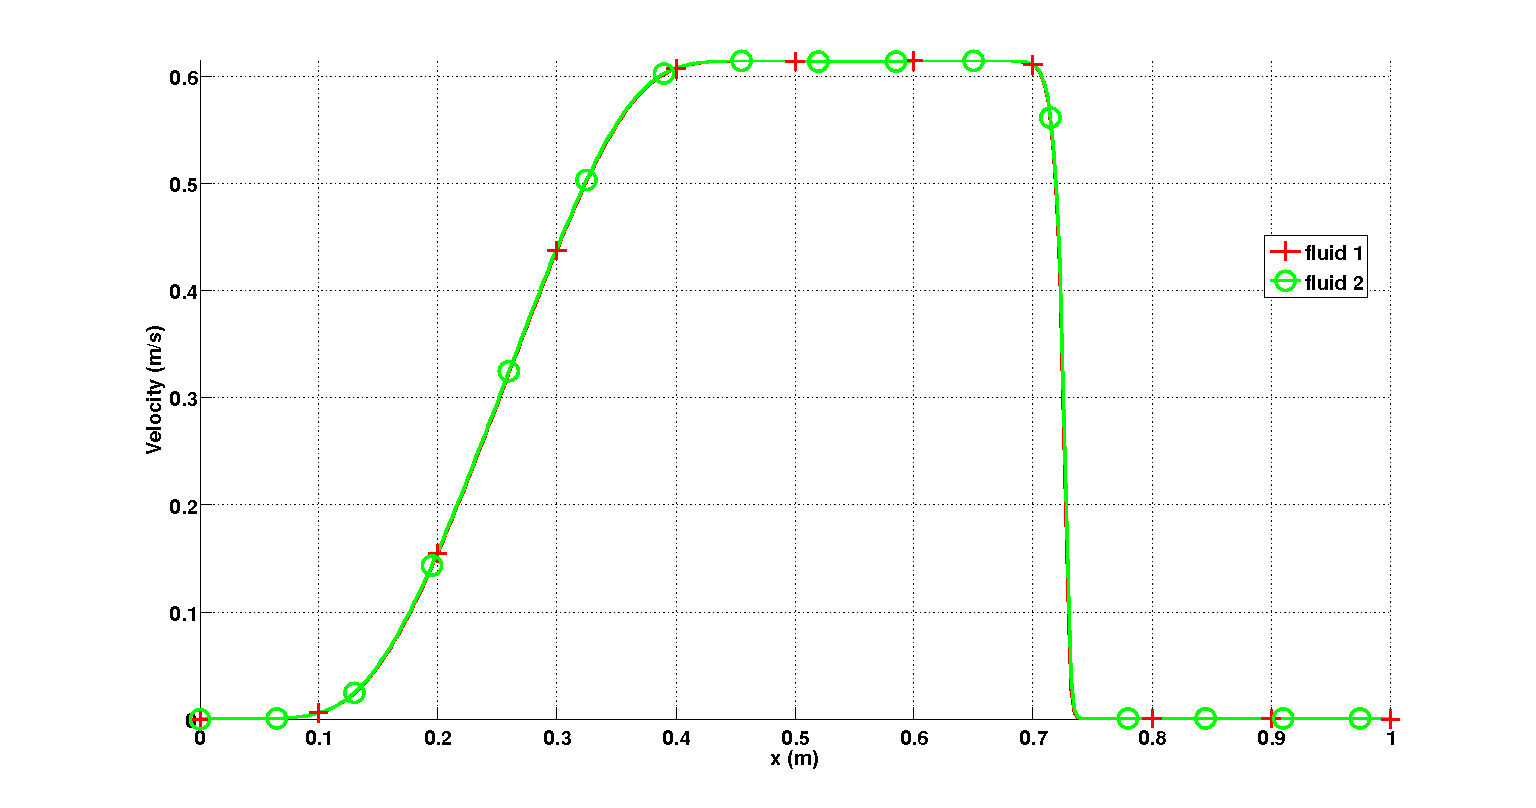
\includegraphics[width=\textwidth]{figures/relaxation_two_phases_velocity_fo_lf.png}
                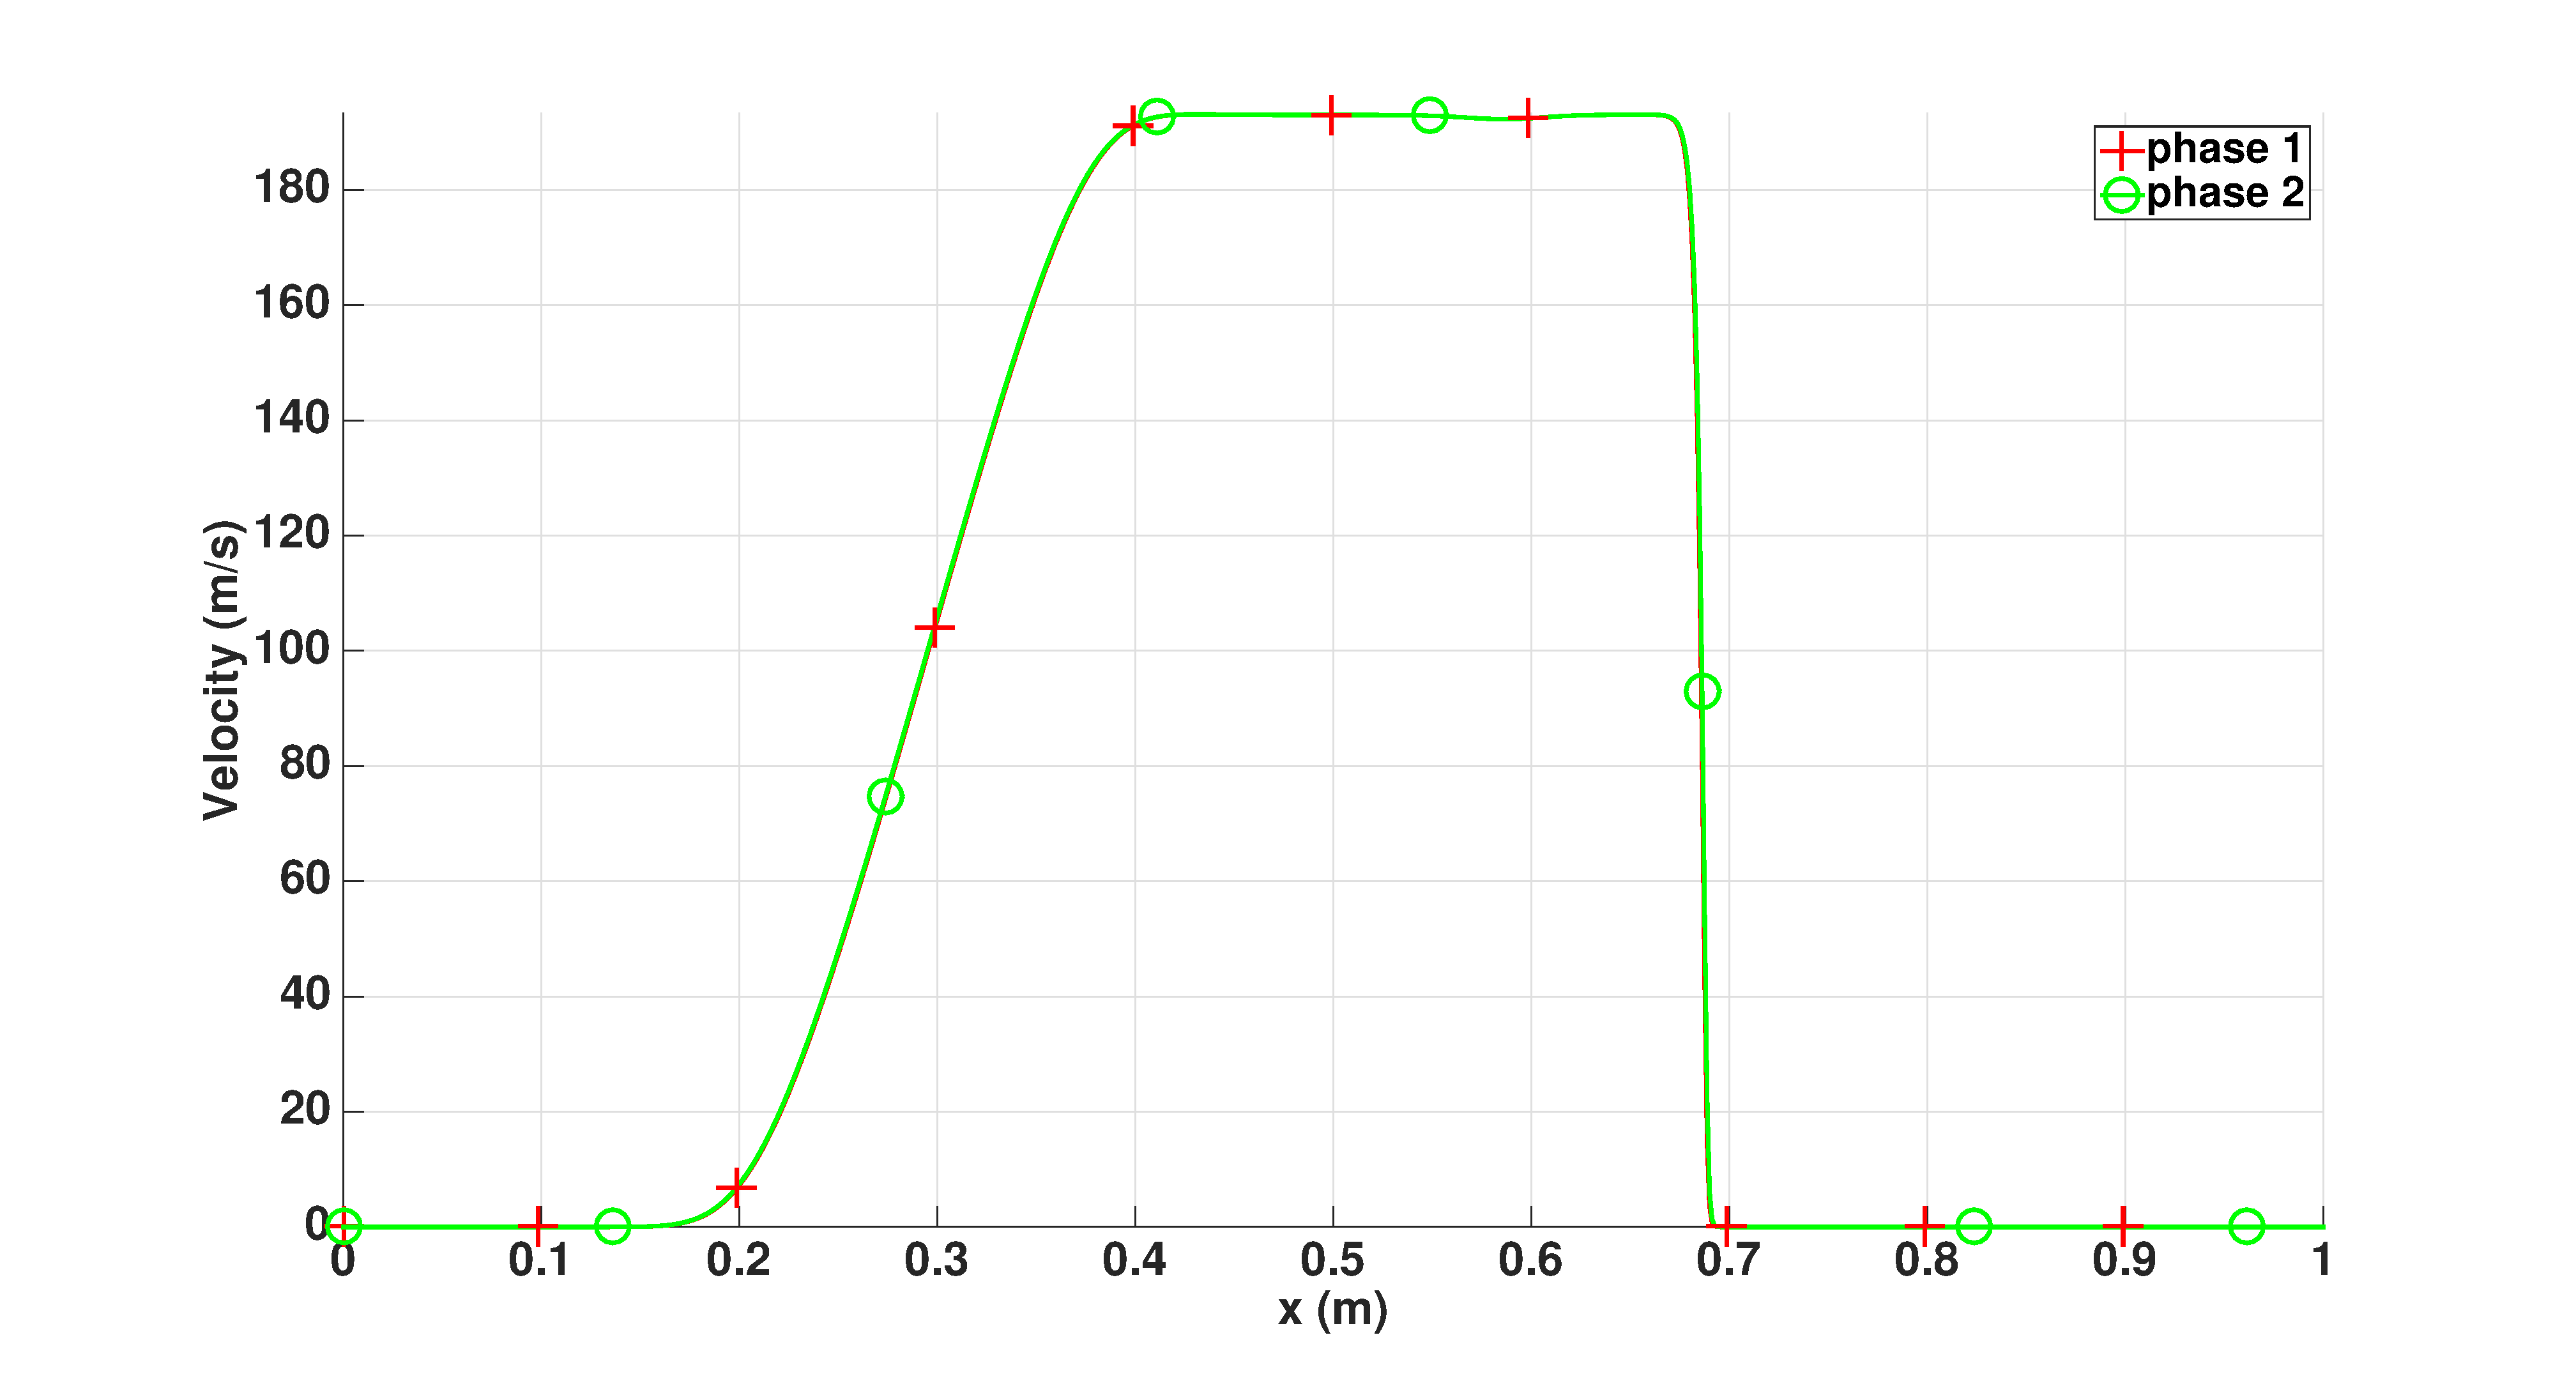
\includegraphics[width=\textwidth]{figures/relaxation_two_phases_velocity.eps}                
                \caption{Velocity}
                \label{fig:two-phase-vel}
        \end{subfigure}%
        \begin{subfigure}[b]{0.5\textwidth}
                \centering
%                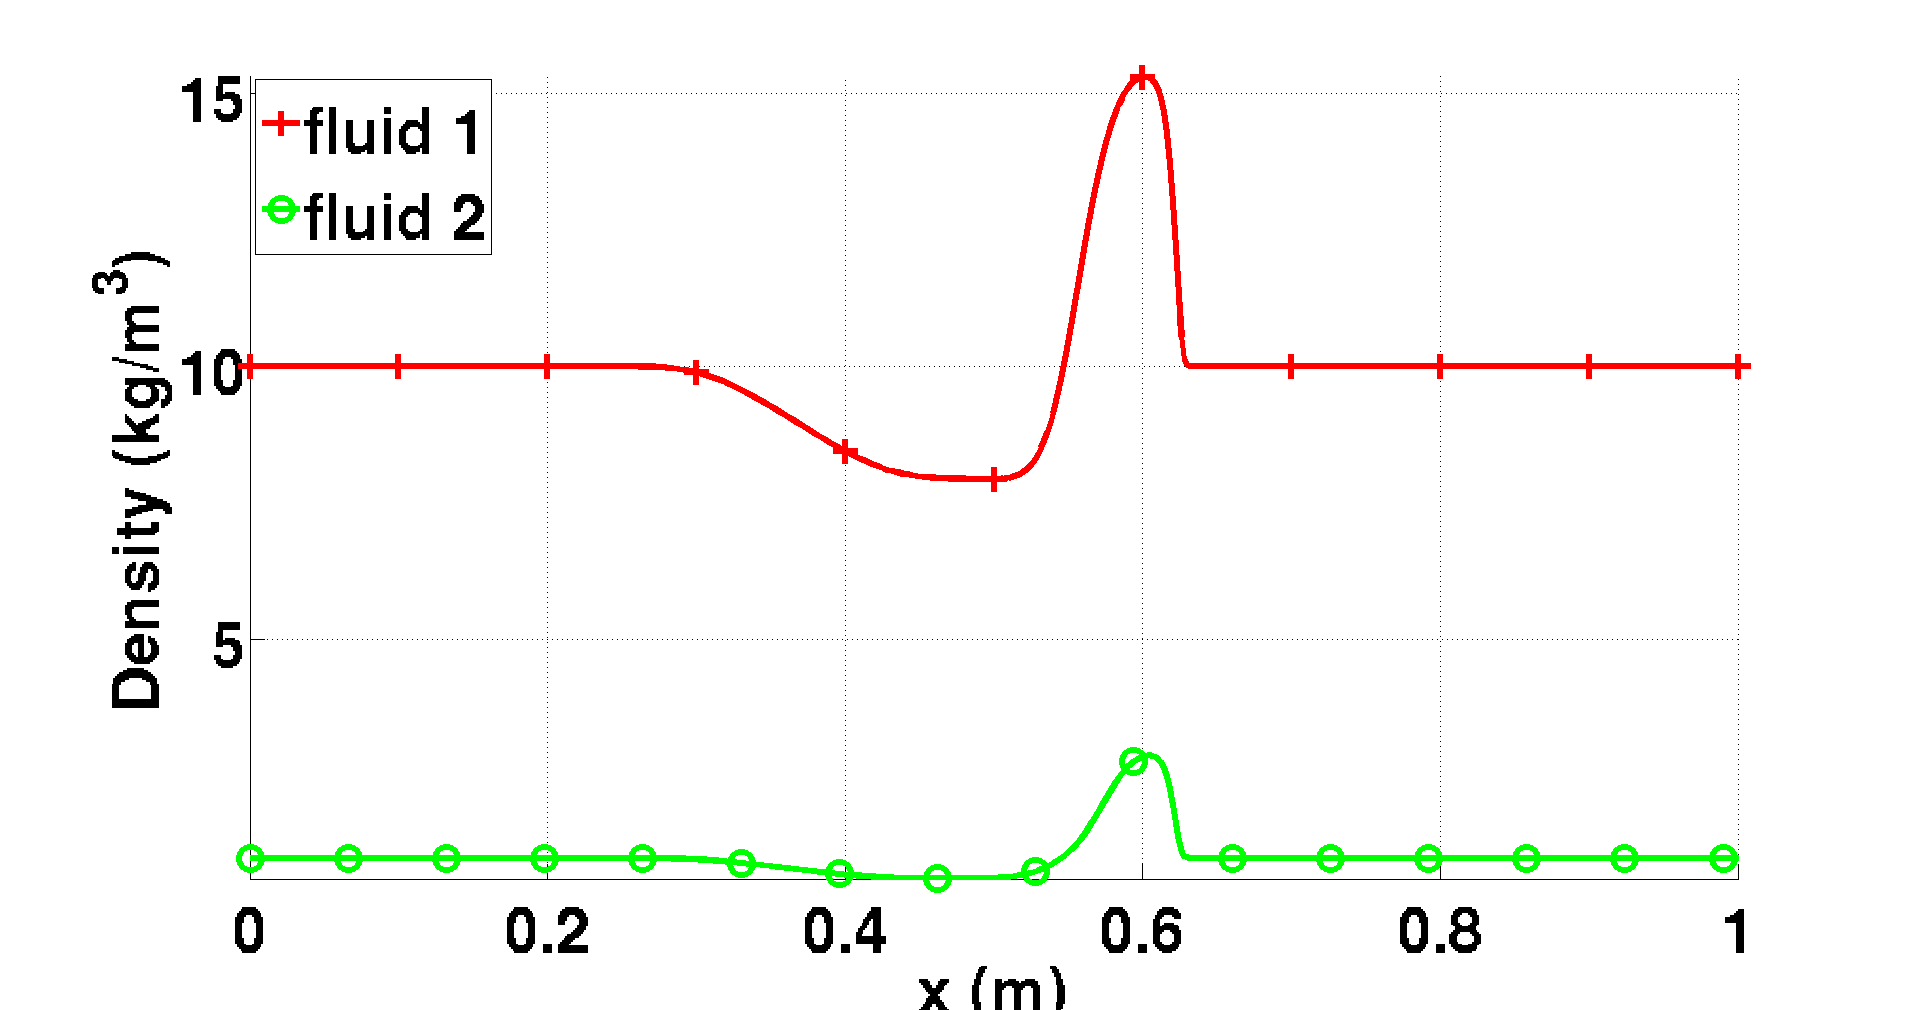
\includegraphics[width=\textwidth]{figures/relaxation_two_phases_density_fo_lf.png}
                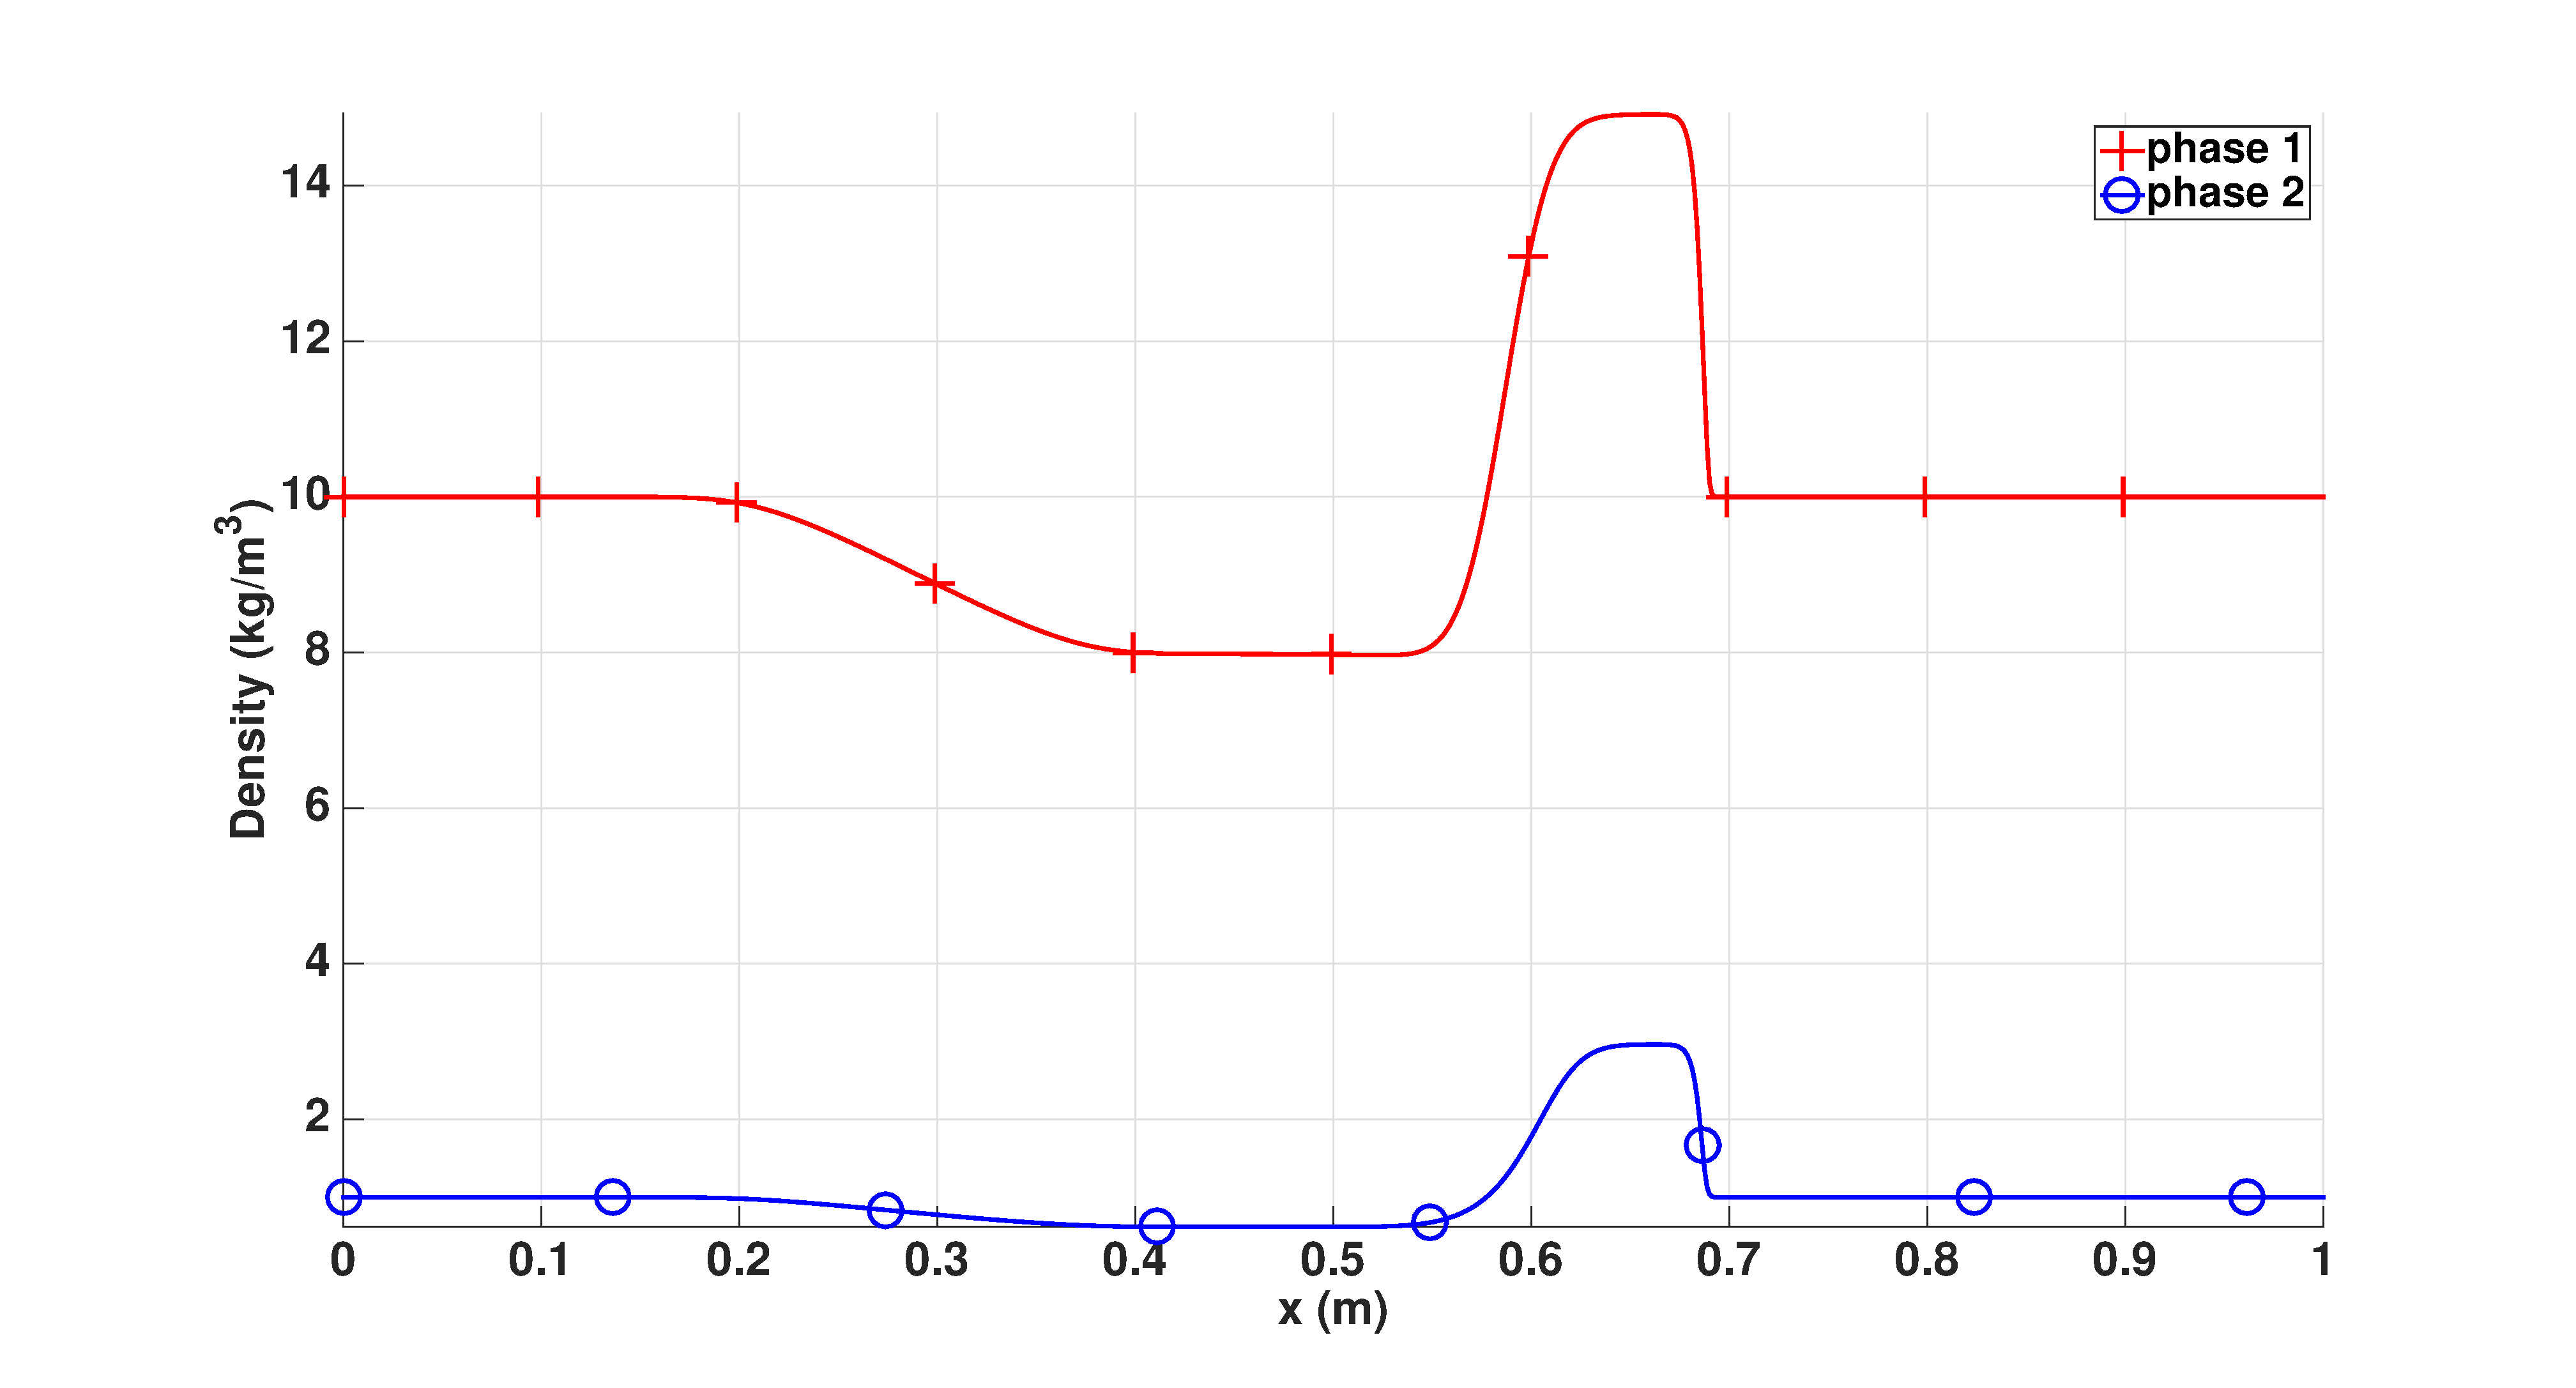
\includegraphics[width=\textwidth]{figures/relaxation_two_phases_density.eps}
                \caption{Density}
                \label{fig:two-phase-density}
        \end{subfigure}
        
        \begin{subfigure}[b]{0.495\textwidth}
                \centering
%                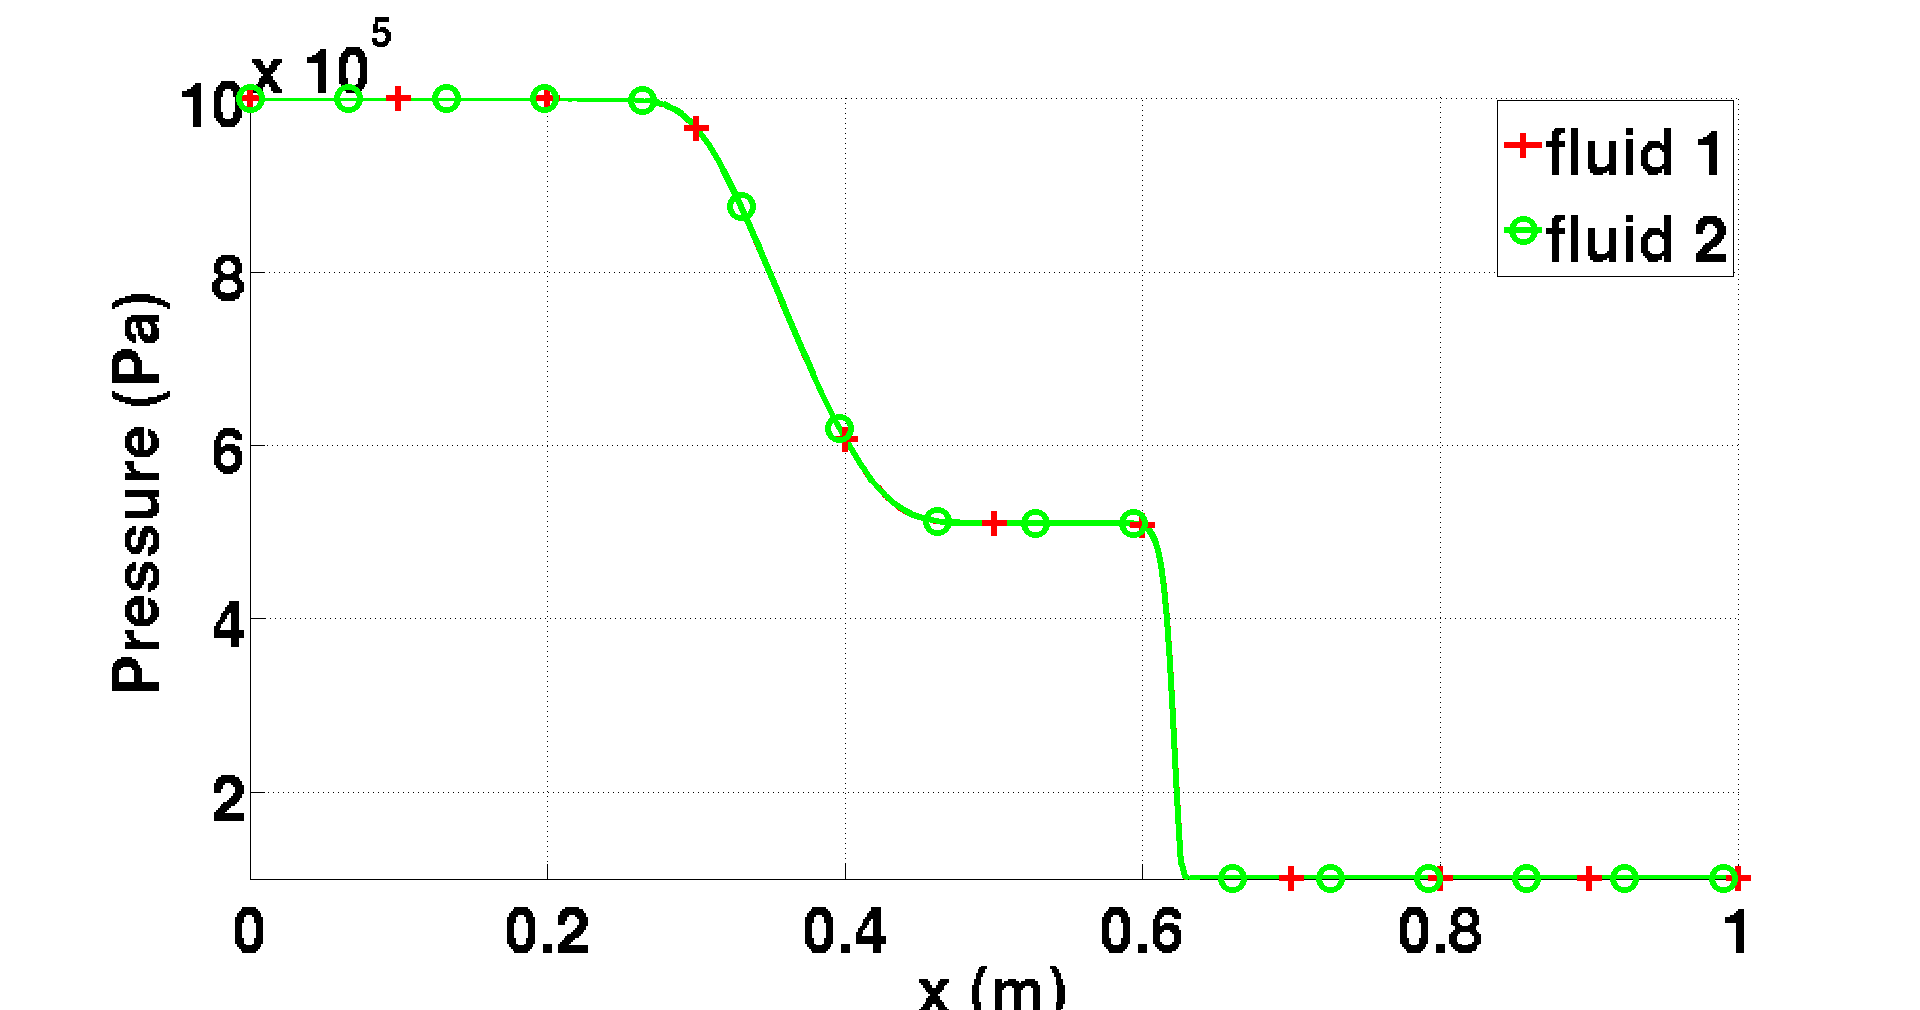
\includegraphics[width=\textwidth]{figures/relaxation_two_phases_pressure_fo_lf.png}
                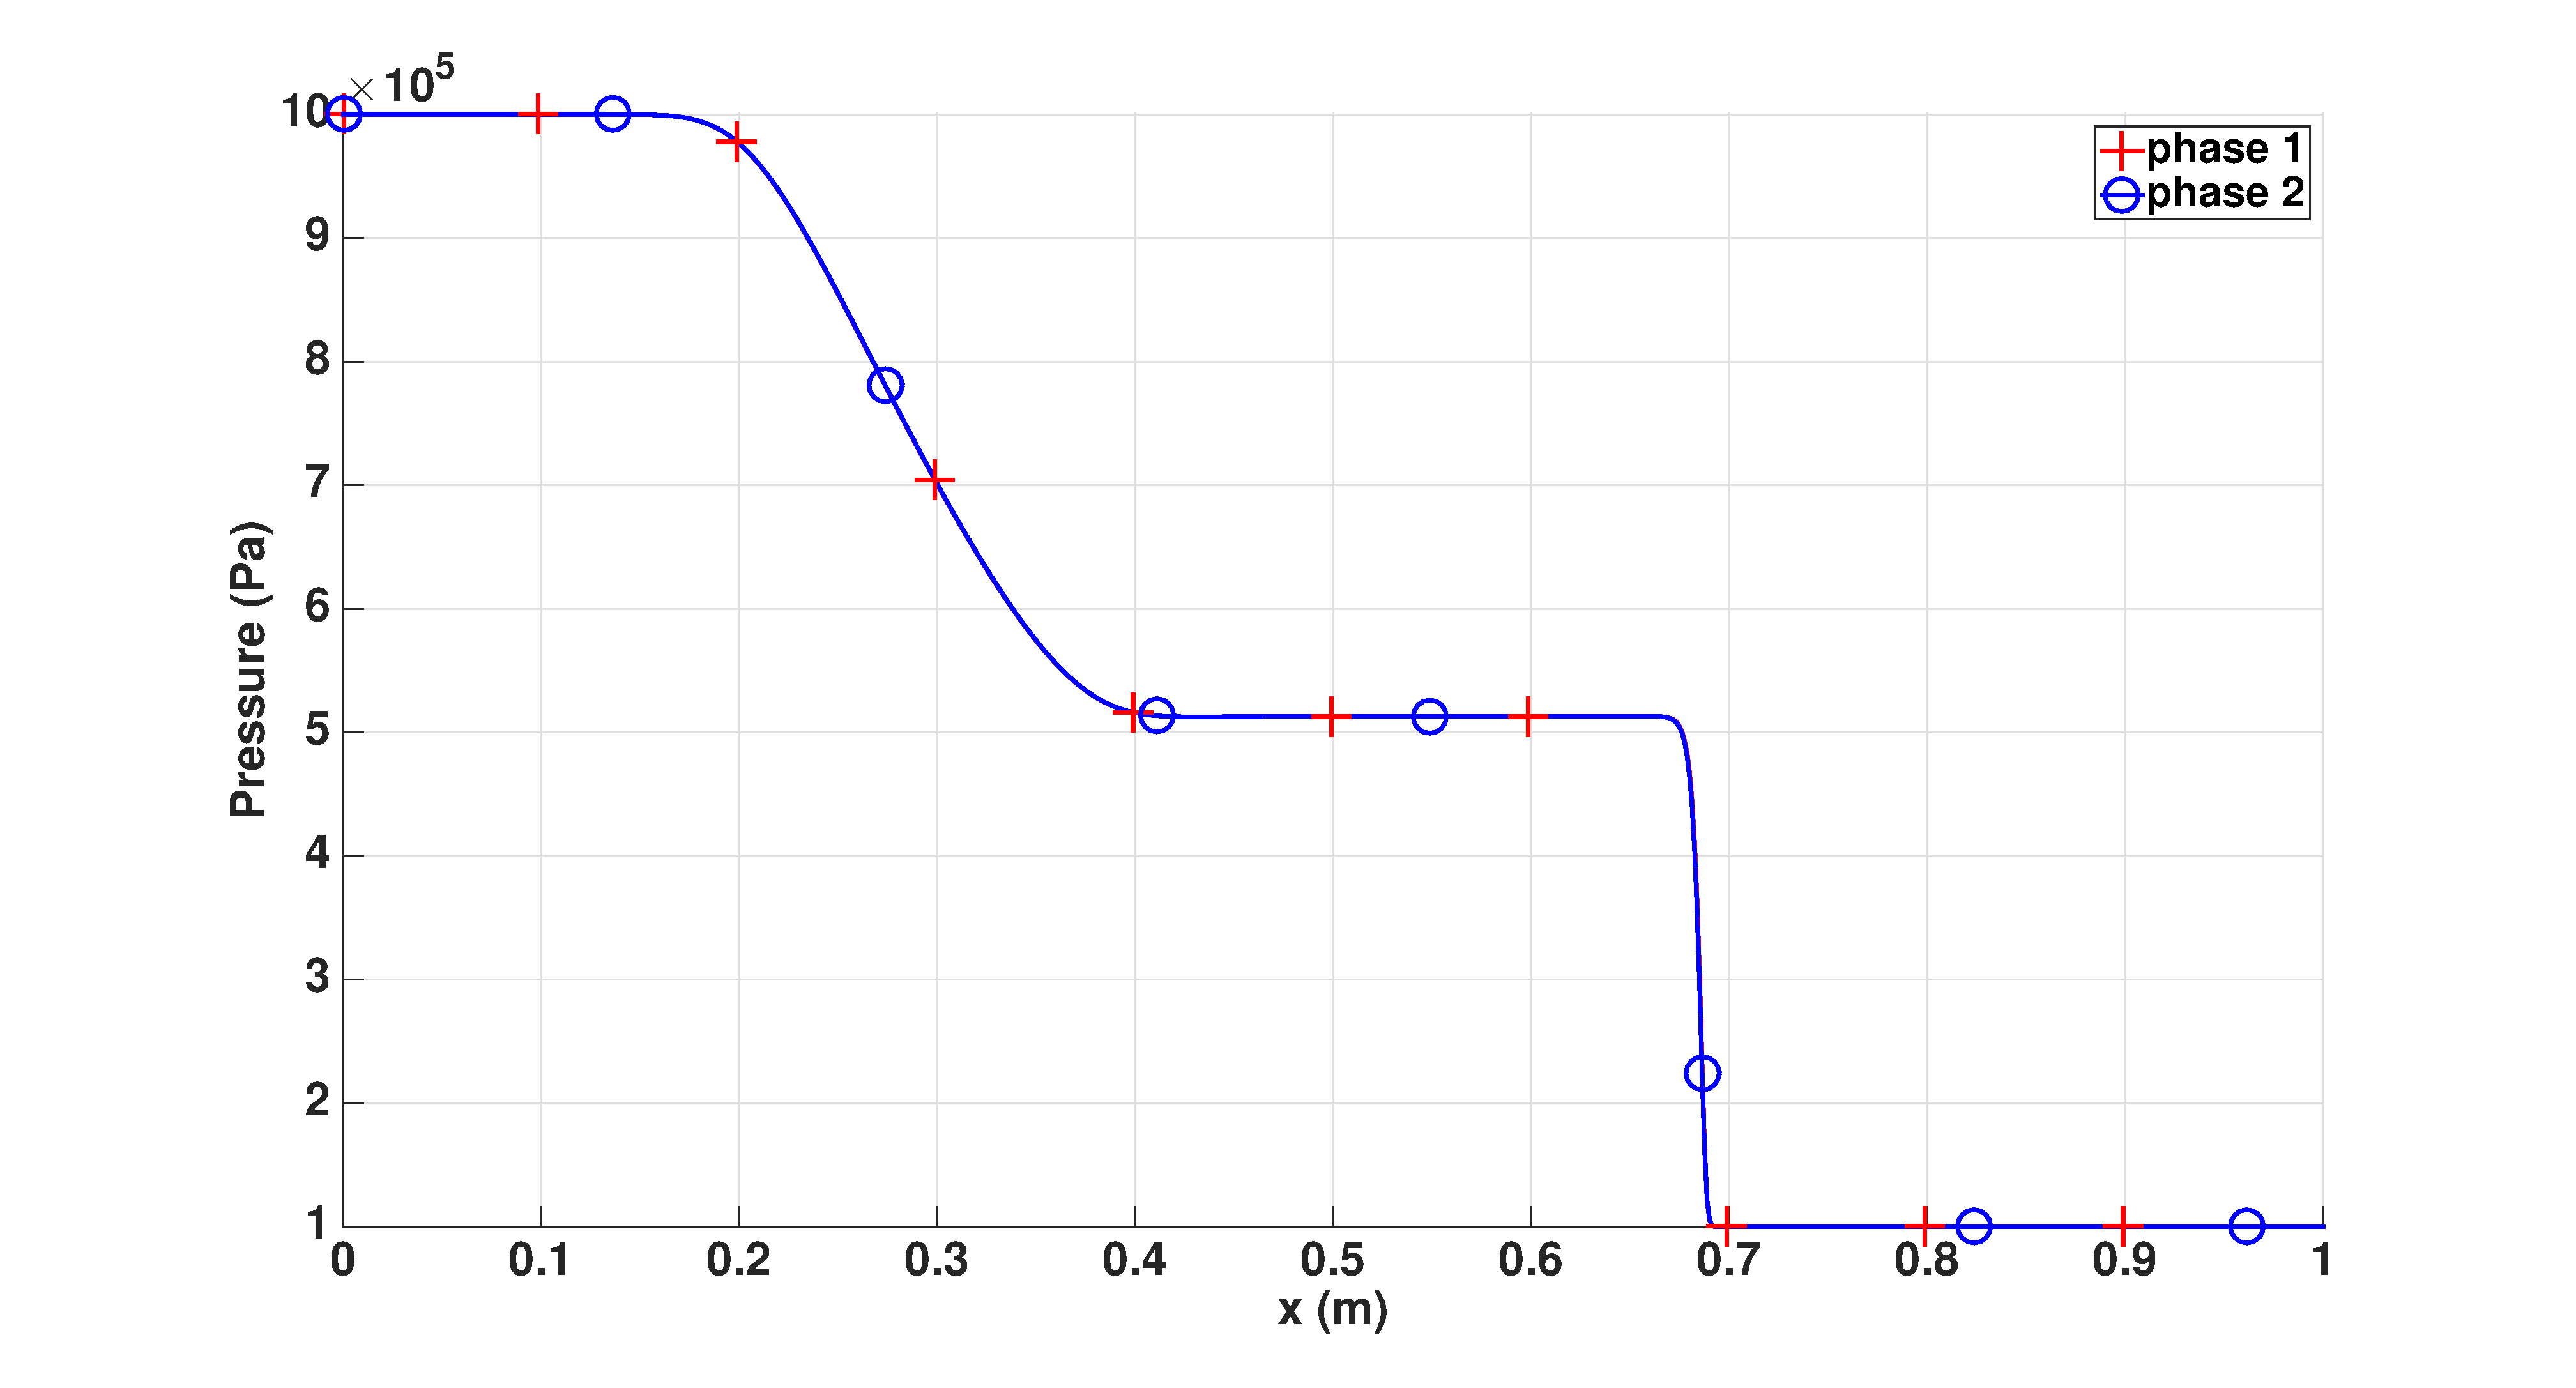
\includegraphics[width=\textwidth]{figures/relaxation_two_phases_pressure.eps}                
                \caption{Pressure}
                \label{fig:two-phase-press}
        \end{subfigure}        
        \begin{subfigure}[b]{0.495\textwidth}
                \centering
%                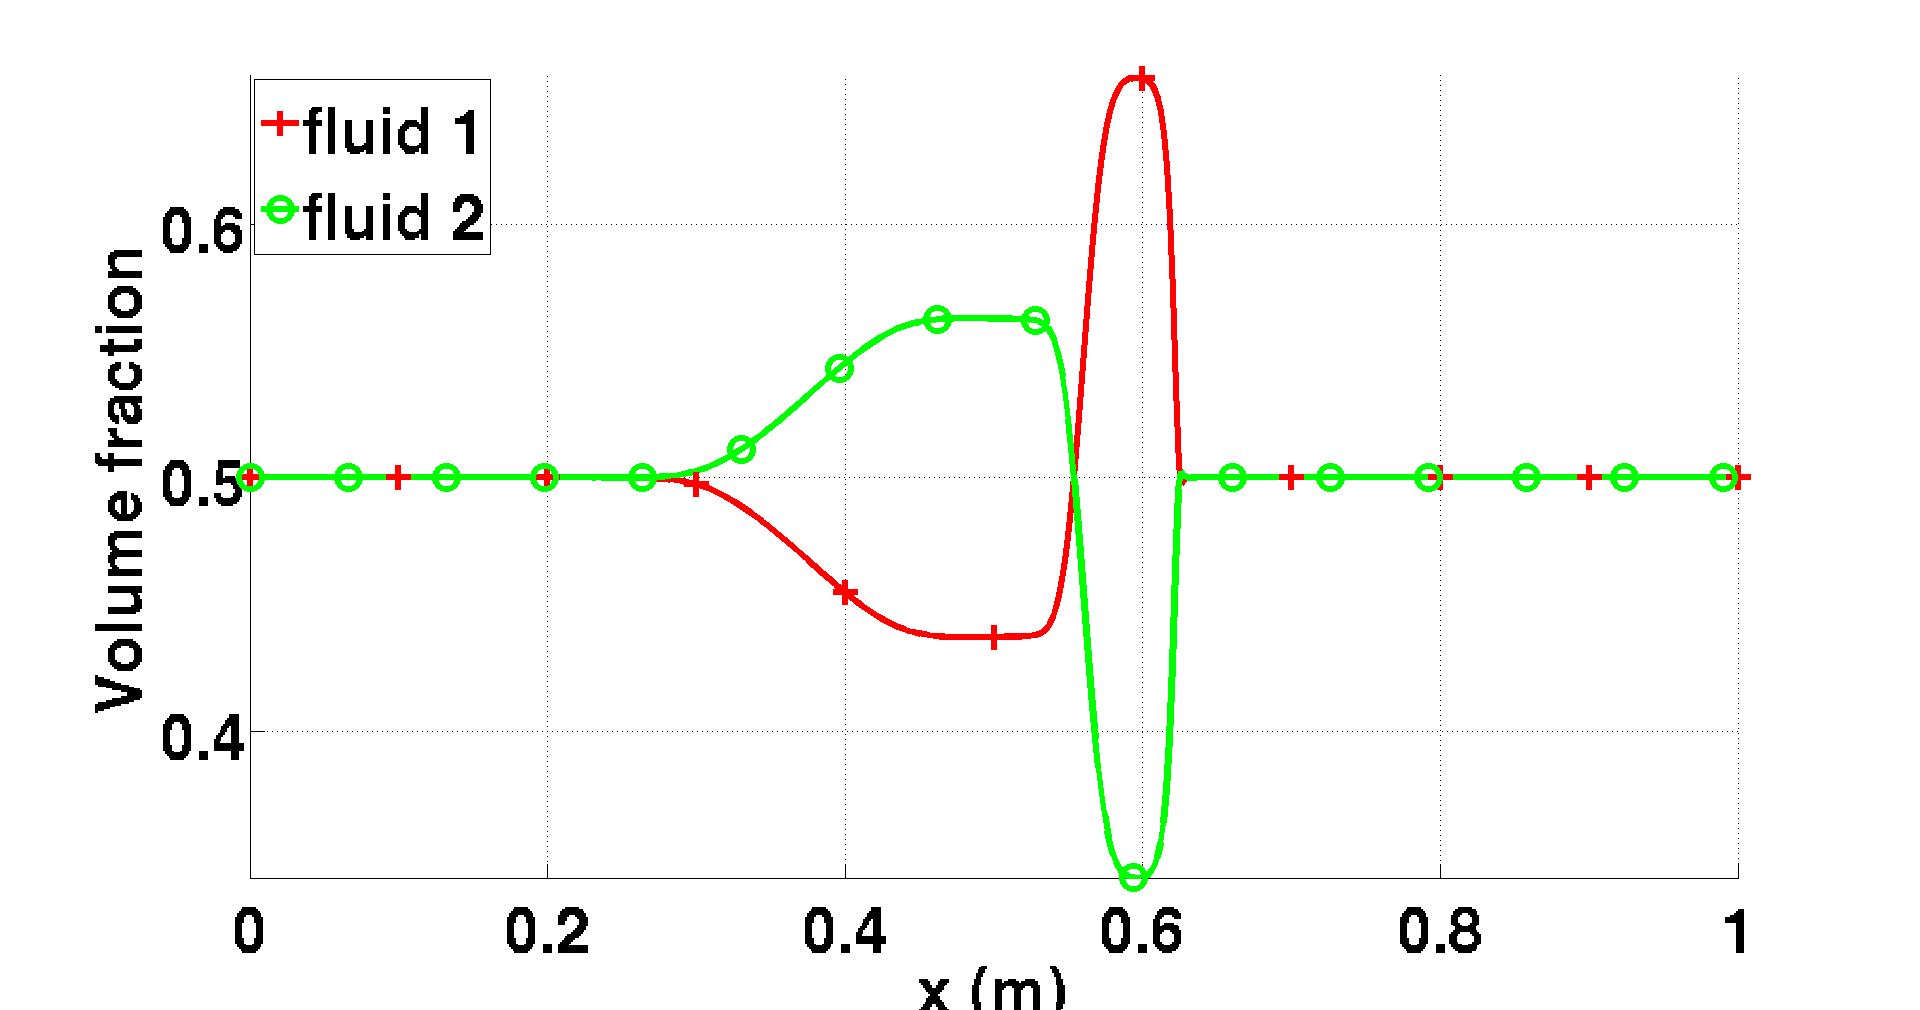
\includegraphics[width=\textwidth]{figures/relaxation_two_phases_volume_fraction_fo_lf.png}
                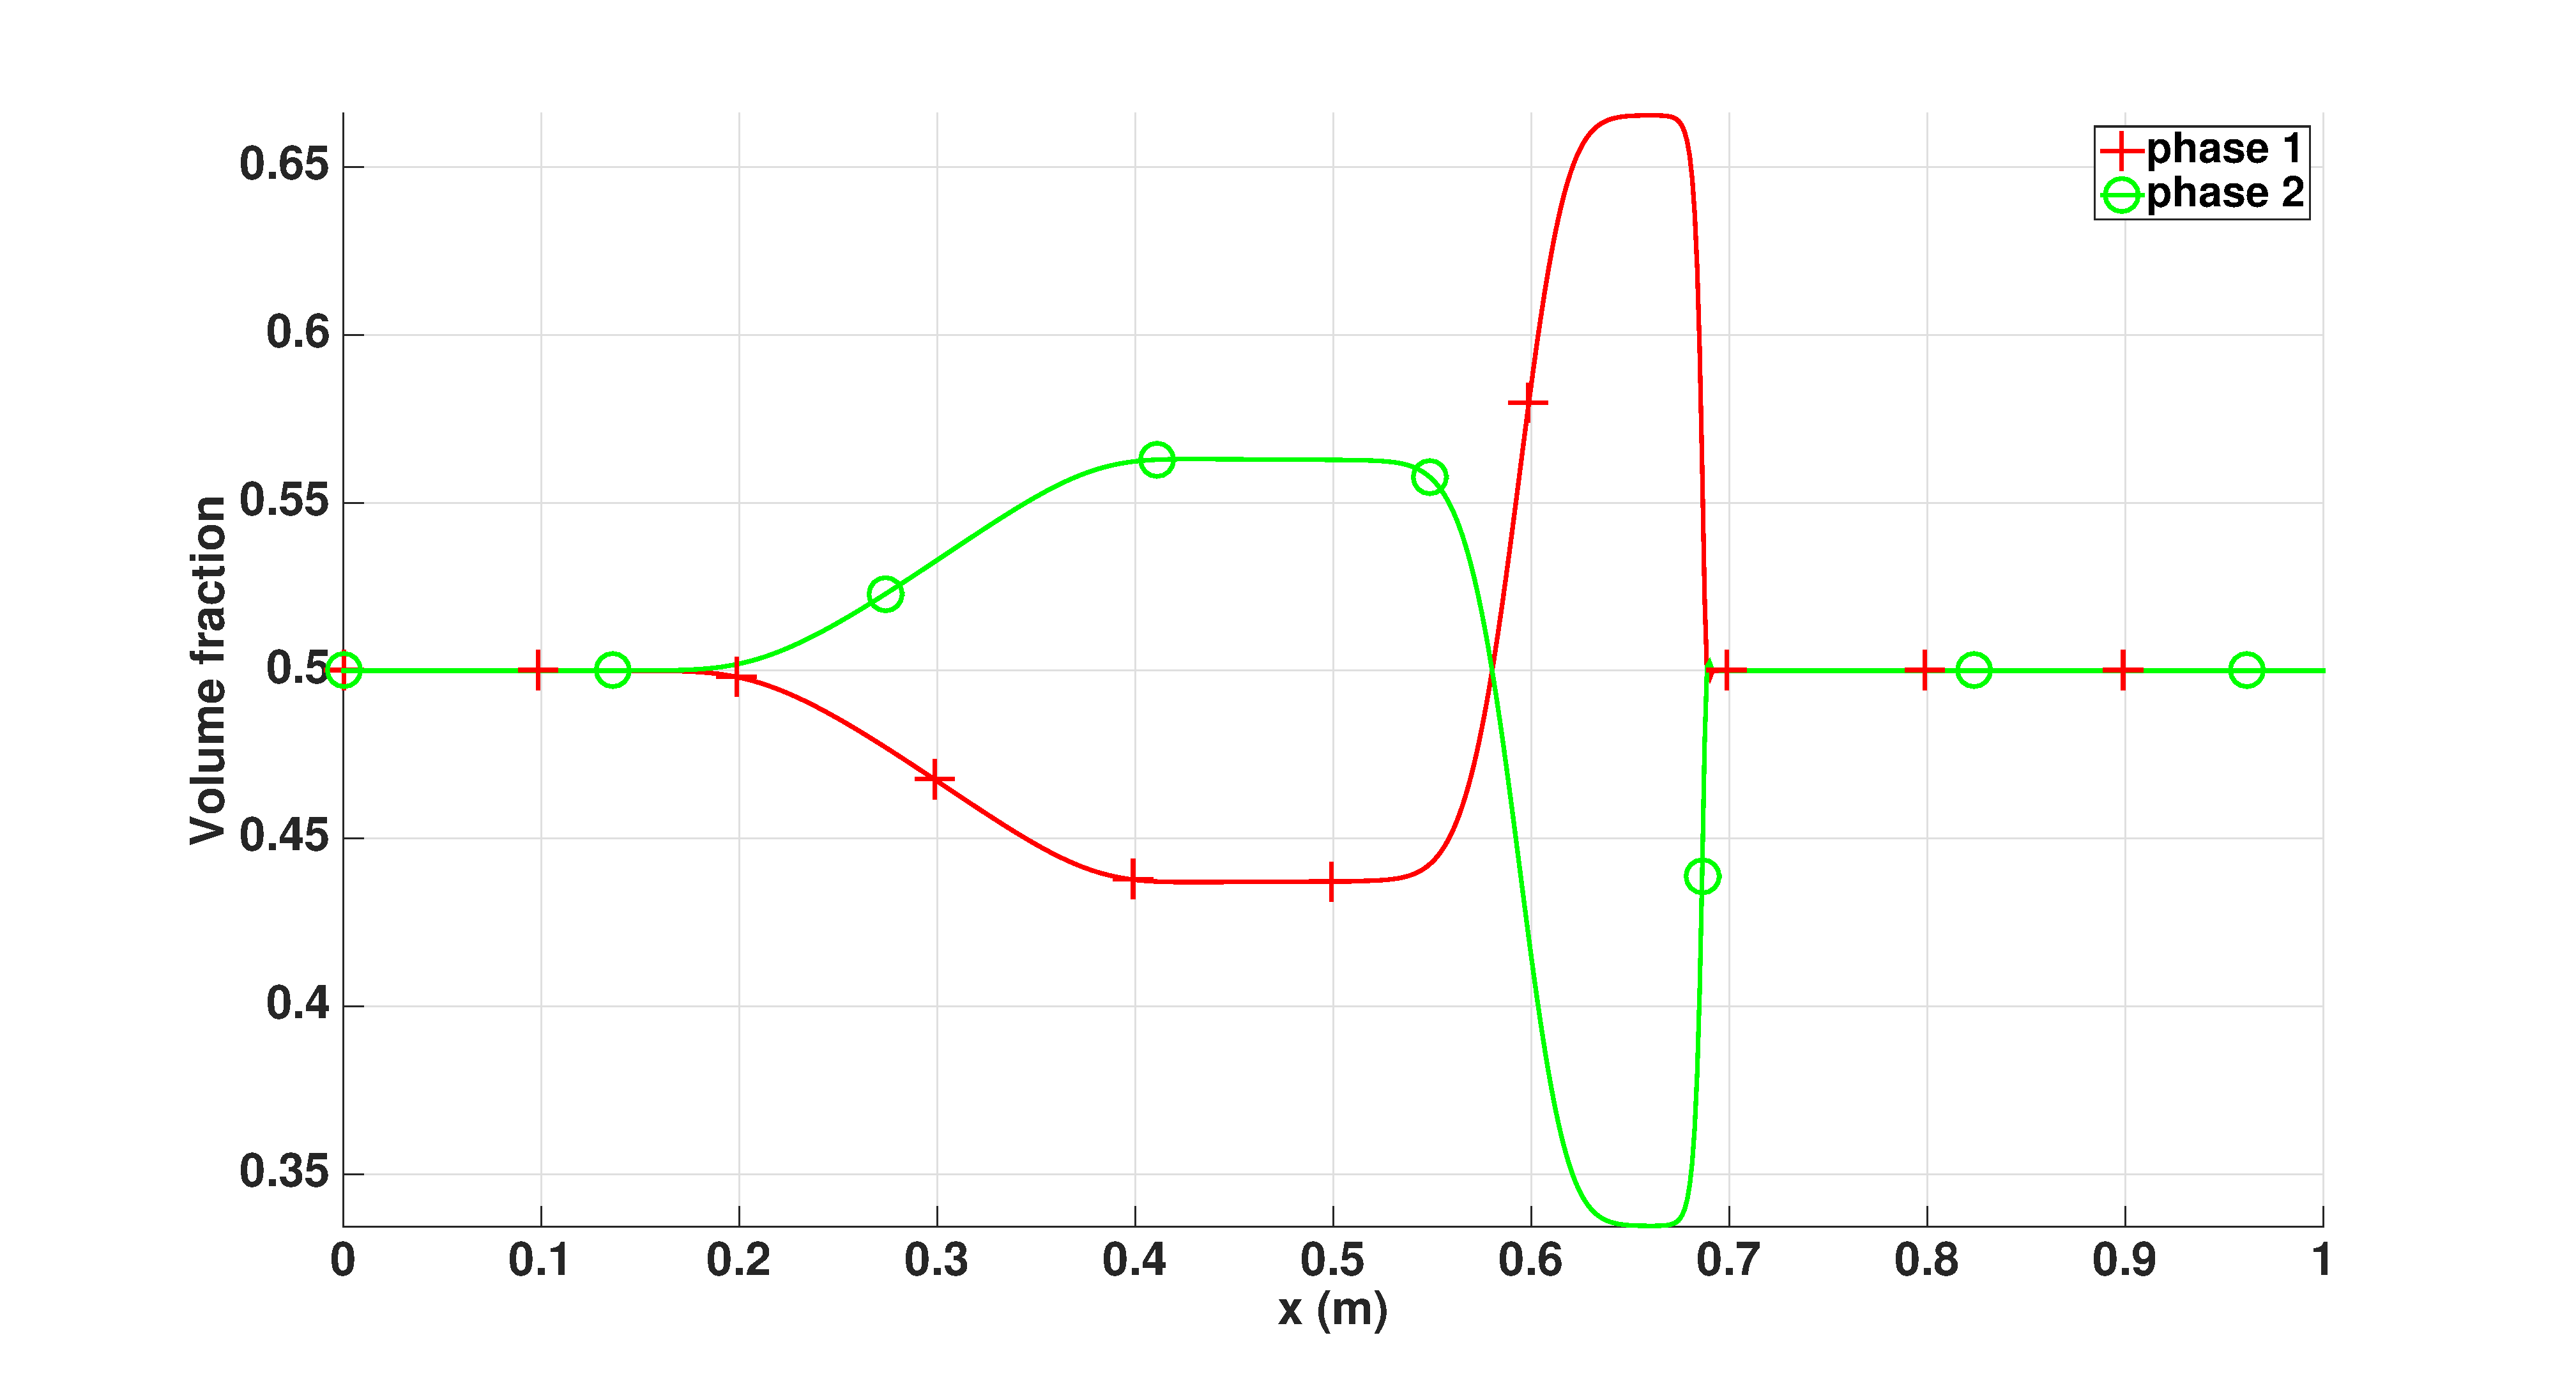
\includegraphics[width=\textwidth]{figures/relaxation_two_phases_volume_fraction.eps}                
                \caption{Volume fraction}
                \label{fig:two-phase-vf}
        \end{subfigure}
        \caption{Two-phase flow shock tube results using a LLF viscosity, ($t=473 \ \mu s$).}\label{fig:two-phase}
\end{figure}
%
The viscous numerical solutions do not display any instability in the vicinity of the shock region ($x \simeq 0.73$ at $t=473 \ \mu s$). In \fig{fig:two-phase-density}, the contact wave ($x \simeq 0.6$) is smeared 
because of the over-dissipative nature of the viscosity coefficients. This example shows that the viscous regularization developed in this paper can efficiently stabilize the numerical solution.
We observe that the phasic pressures and velocities are indeed identical for large values of the relaxation parameters.
%This example demonstrates the ability of the proposed viscous regularization to stabilize the seven-equation two-phase flow model.
%
%------------------------------------------------------------
\subsubsection{A grid-convergence study}\label{sec:grid-conv-study}
 %------------------------------------------------------------
 %
The proposed regularization is grid-dependent, i.e., the phasic viscosity coefficients are set proportional to the grid size $h$. Thus, it is of interest to investigate the behavior of the numerical solution as the mesh is refined, especially in the
vicinity of the contact (around $x=0.6$) and shock (around $x=0.7$) waves where the use of a LLF viscosity led to excessive smearing as shown in the density and the volume fraction profiles in \fig{fig:two-phase-density} and 
\fig{fig:two-phase-vf}, respectively. Thus, we propose to run the same test as before using three different mesh resolutions:
 200, 400 and 800 cells. The numerical solutions of the phasic densities and the phasic volume fractions obtained are displayed
in \fig{fig:density-mult-meshes} and \fig{fig:vf-mult-meshes}, respectively.
%
\begin{figure}[H]
        \centering
        \begin{subfigure}[b]{0.95\textwidth}
                \centering
                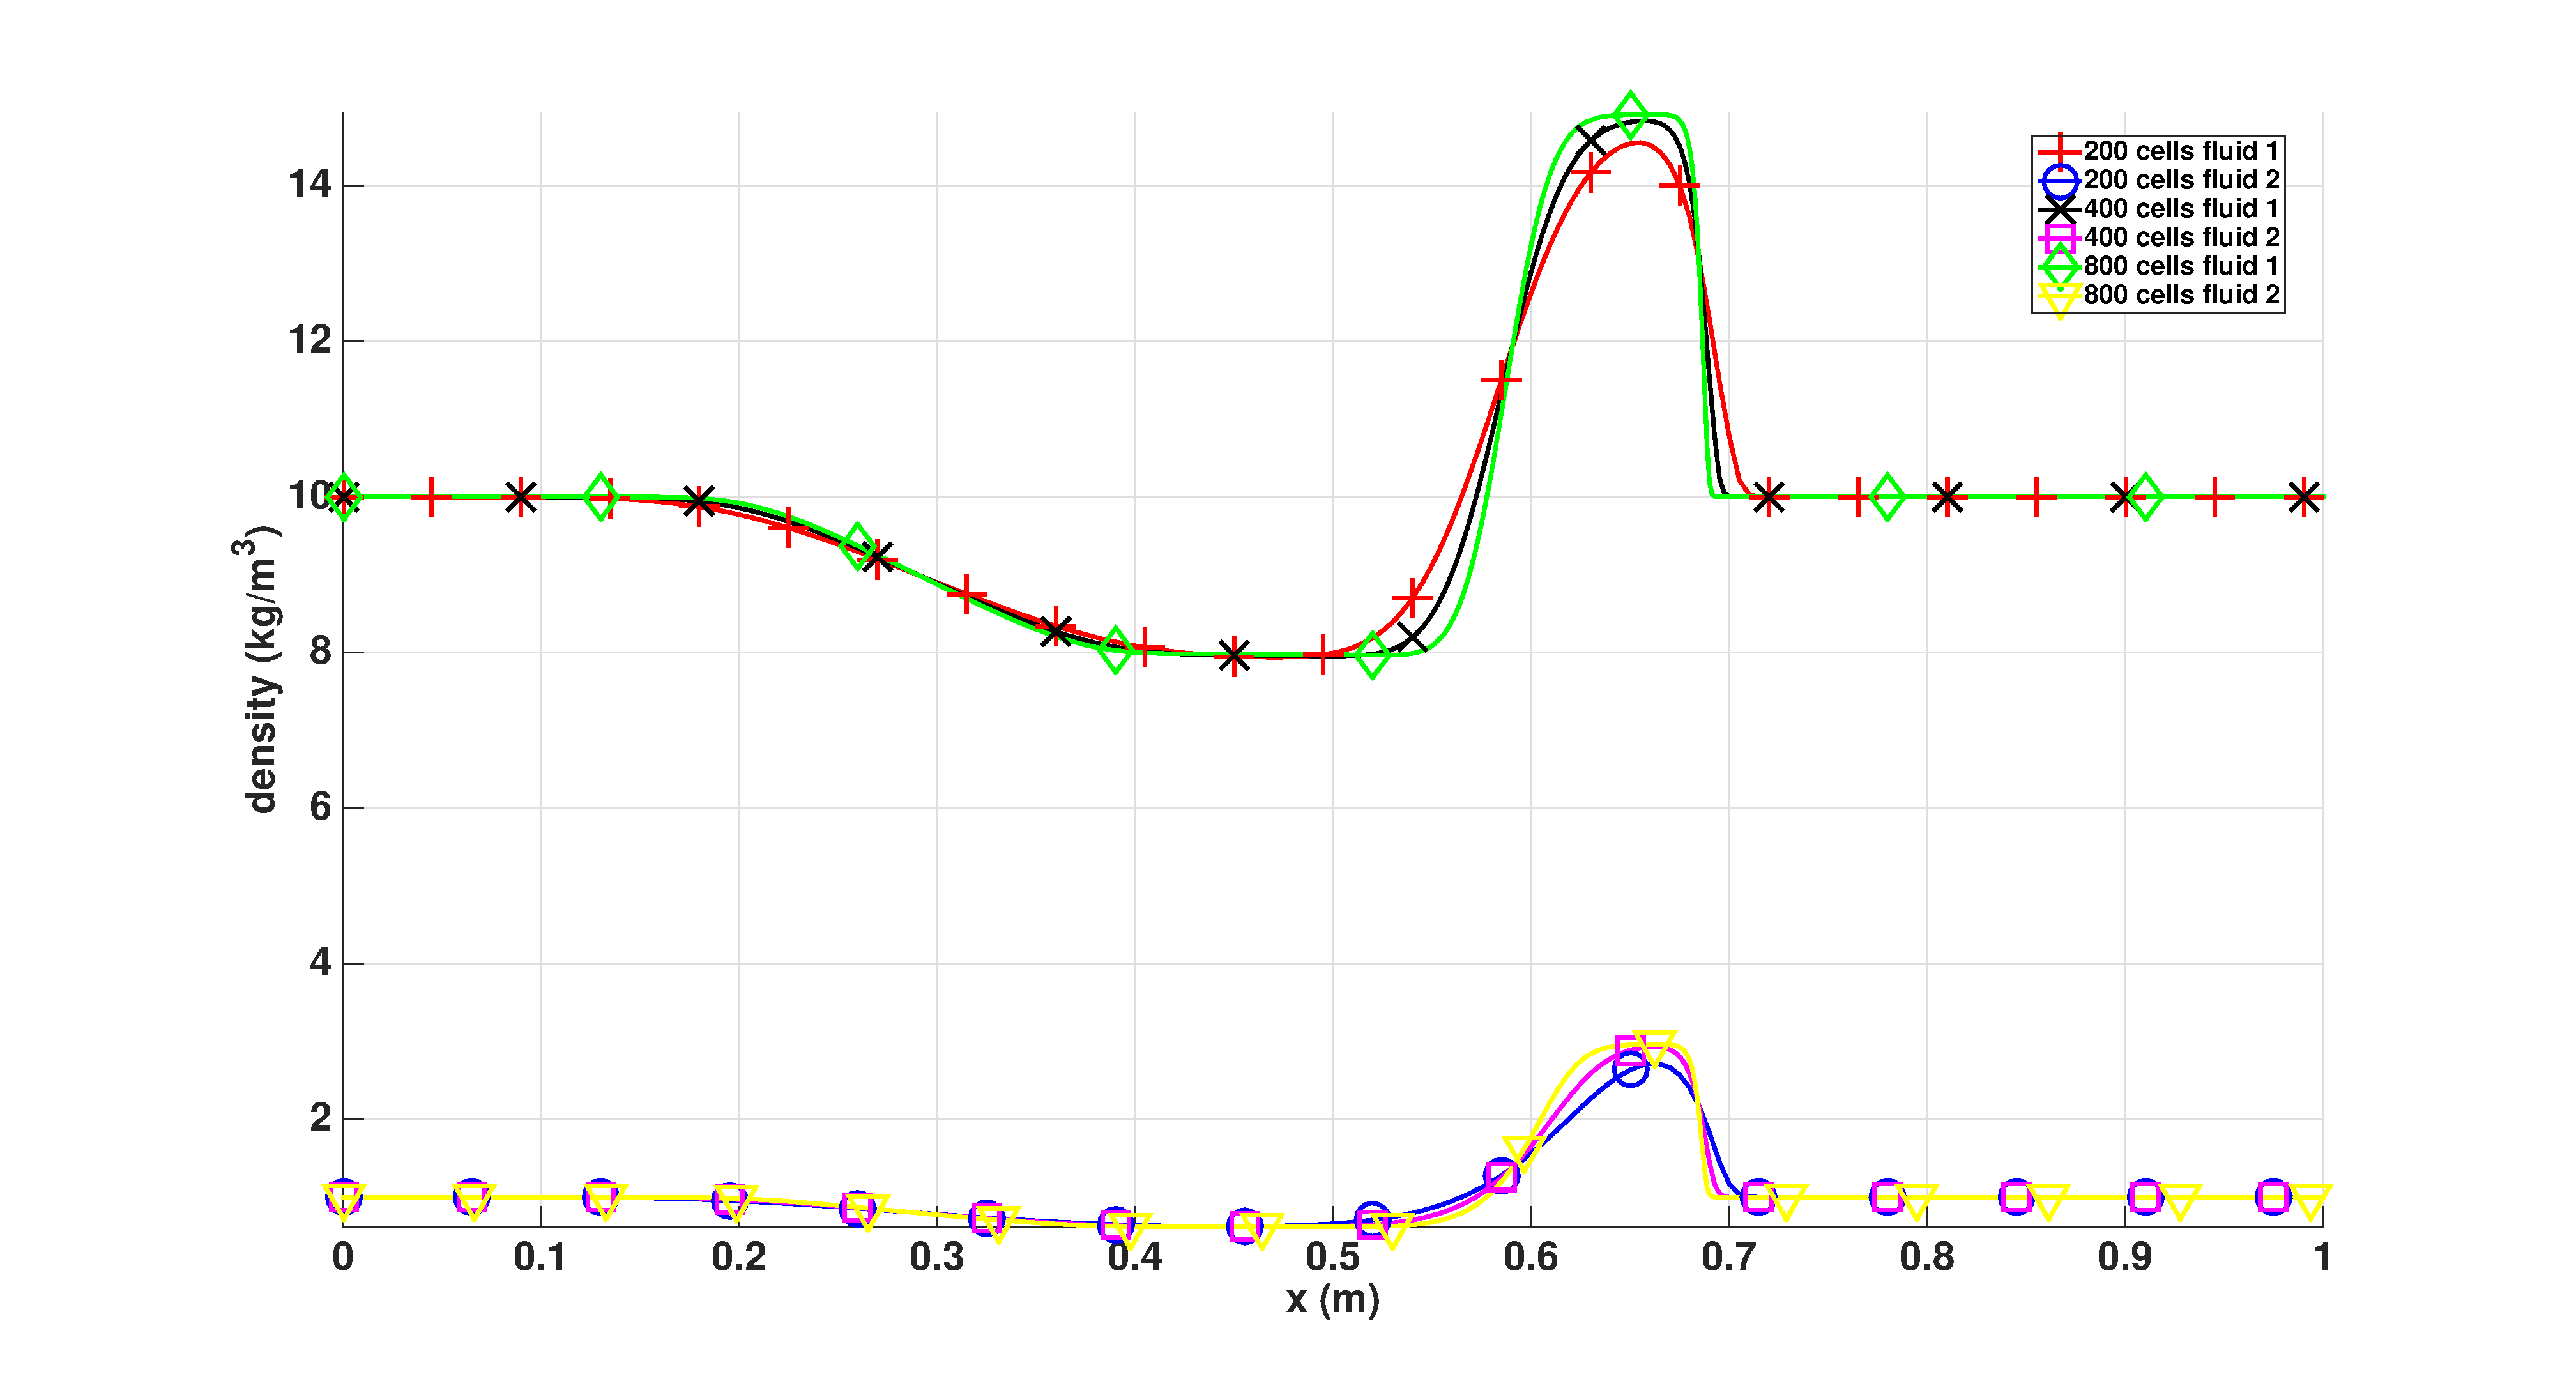
\includegraphics[width=\textwidth]{figures/relaxation_two_phases_density_multi_mesh.eps}
                \caption{Density.}
                \label{fig:density-mult-meshes}
        \end{subfigure}
				\\
        \begin{subfigure}[b]{0.95\textwidth}
                \centering
                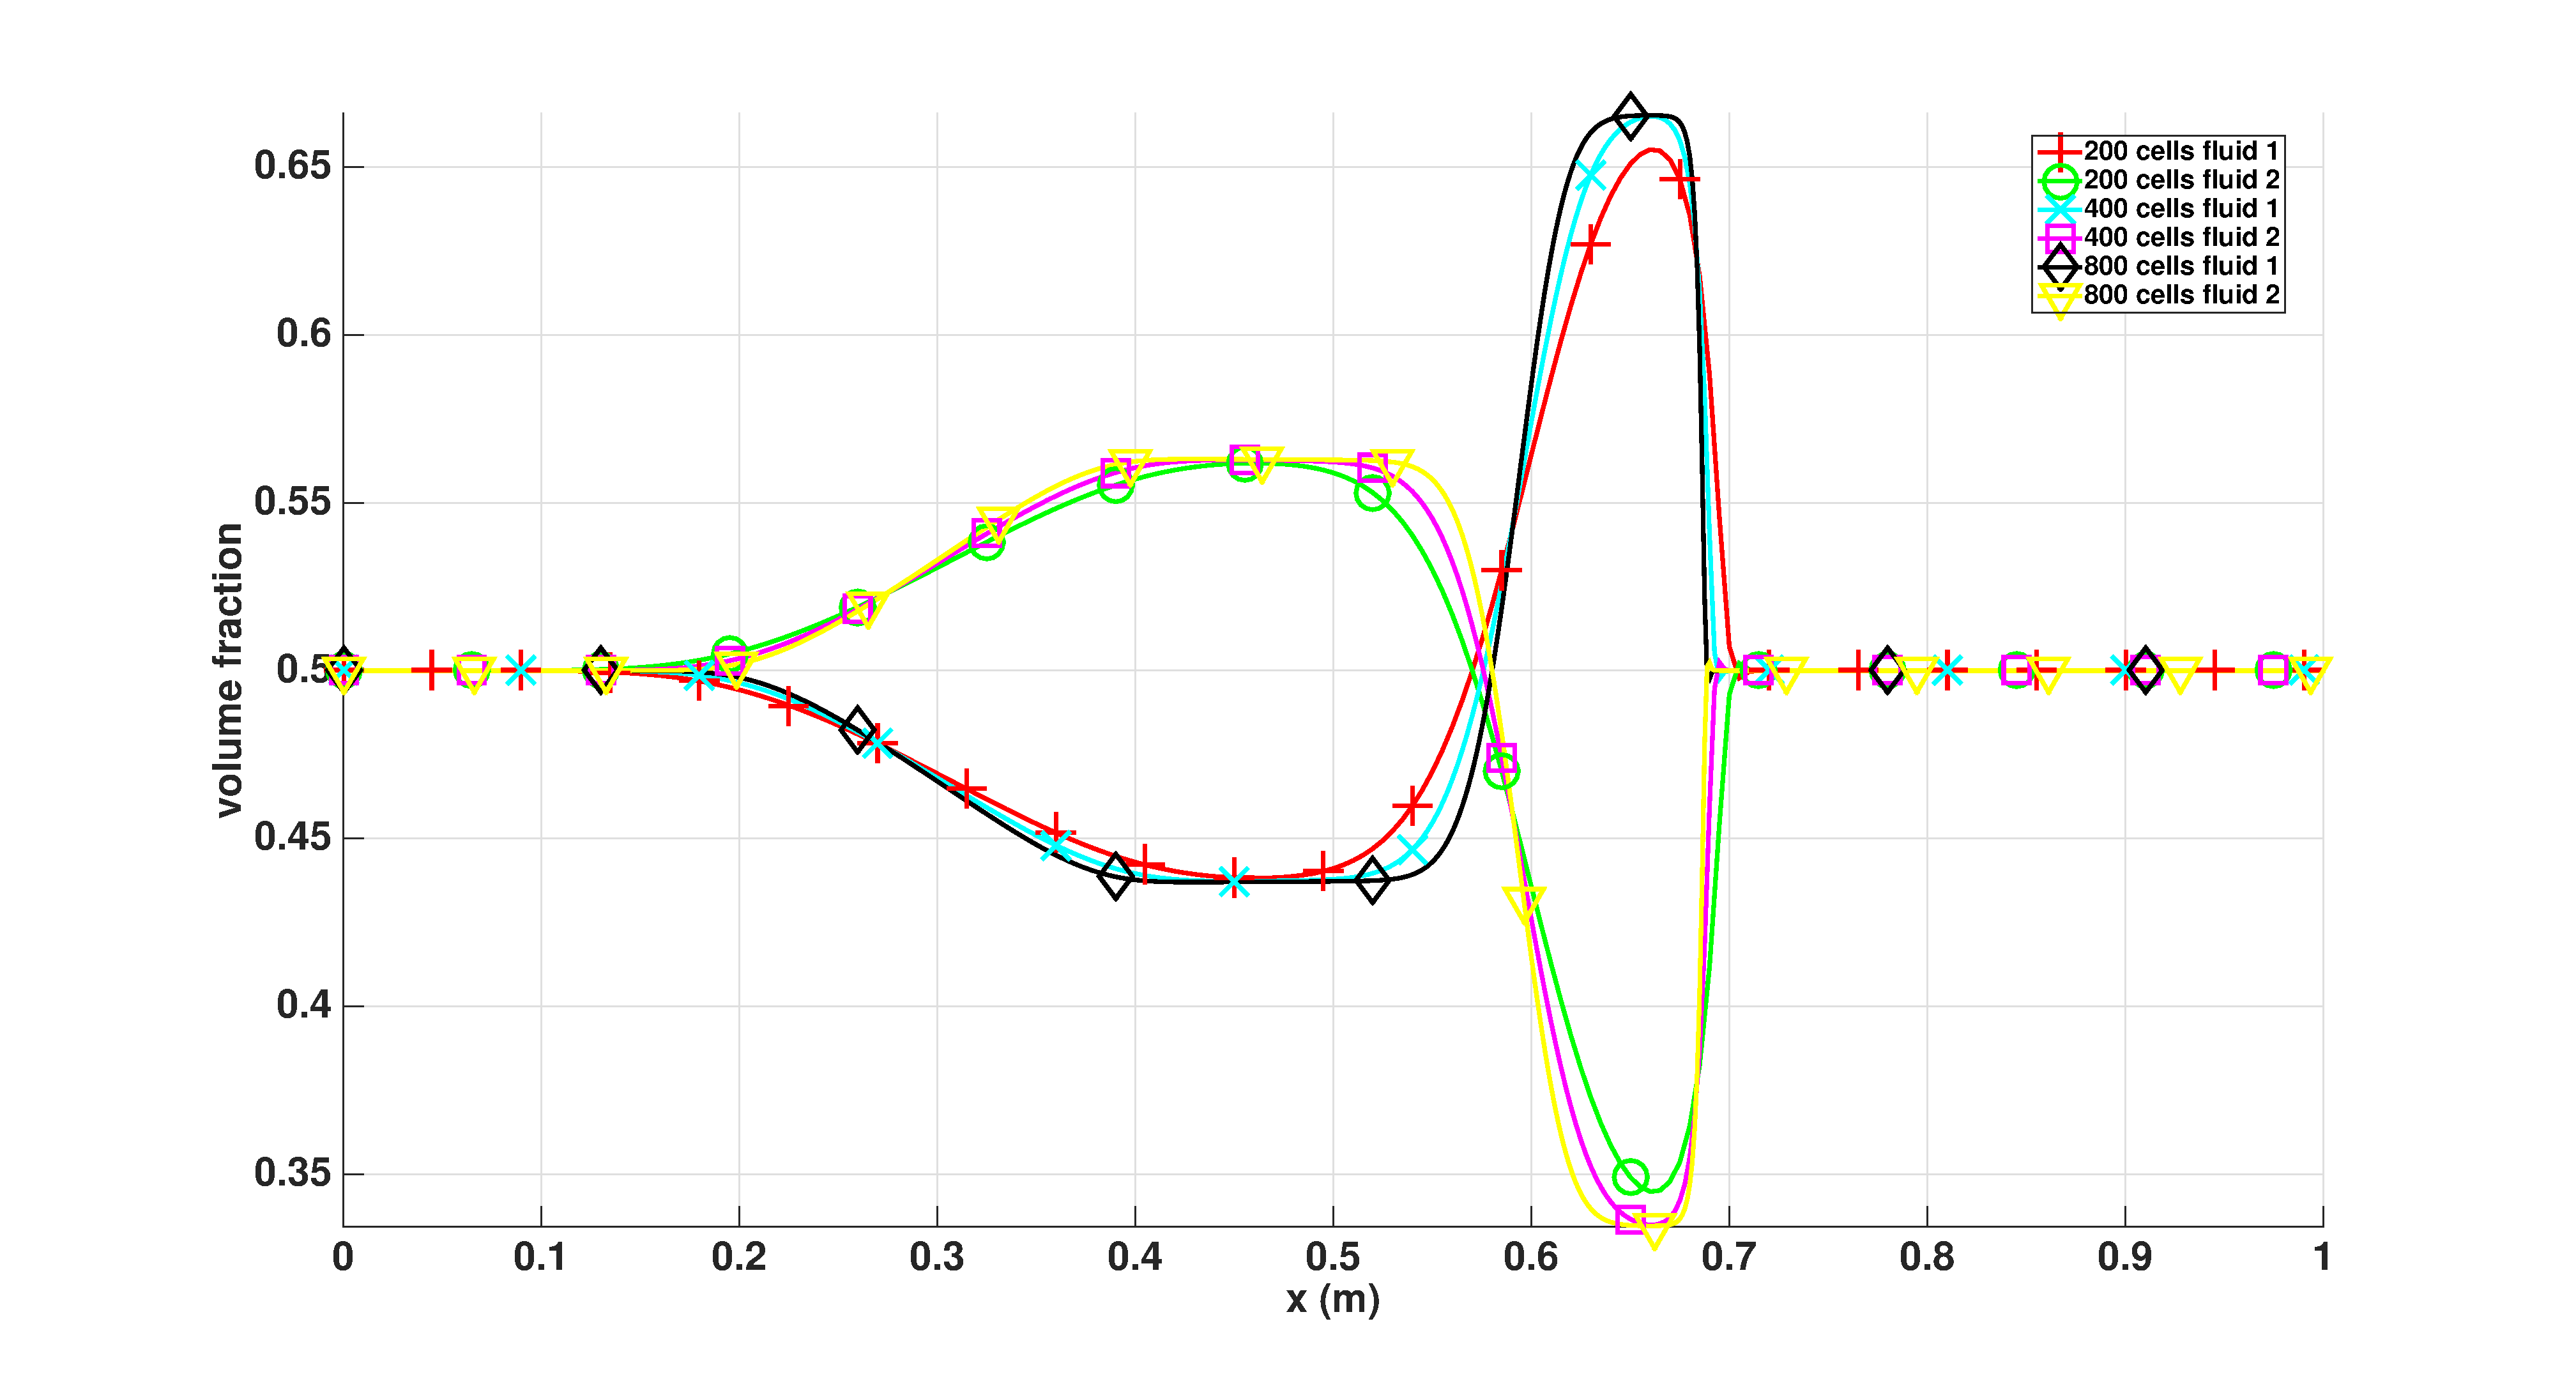
\includegraphics[width=\textwidth]{figures/relaxation_two_phases_volume_fraction_multi_mesh.eps}
                \caption{Volume fraction.}
                \label{fig:vf-mult-meshes}
        \end{subfigure}
        \caption{Two-phase flow shock tube results using a LLF viscosity, mesh refinement study ($t=473 \ \mu s$).}
				\label{fig:density-vf-mult-mesh}
\end{figure}
%
From the phasic density profiles in \fig{fig:density-mult-meshes}, it is observed that the contact and the shock waves are better resolved as the mesh is refined, as expected, indicating that the numerical solution converges, at least formally, to a weak solution. Similar observations can be drawn for the phasic volume fraction profiles, as shown in \fig{fig:vf-mult-meshes}, and were also observed for the other phasic variables, i.e., pressure and velocity (not shown).
%
%------------------------------------------------------------
\subsubsection{Numerical solutions with an incomplete viscous regularization}\label{sec:incompete-visc-reg}
 %------------------------------------------------------------
 %
In this test, we investigate the influence of regularizing some or all of the equations on the numerical solution, as an illustration 
of \rmk{rmq:rmq_vf_diss_term}. %and \rmk{rmq:rmq_cont_diss_term}:
We use again the previous shock test case and select the LLF viscosity and consider the following 3 cases:
%
\begin{enumerate}
\item all viscosity coefficients non zero, i.e., the local Lax-Friedrichs scheme already shown in \fig{fig:two-phase} (viscosity type 1), 
\item the definitions for $\mu_k$ and $\kappa_k$ are unchanged but $\beta_k$ is set to zero (viscosity type 2). In doing so, we assess the effect of the viscous stabilization on the volume fraction, and 
\item the viscosity coefficients $\kappa_k$ and $\beta_k$ are set to zero while $\mu_k$ is unchanged (viscosity type 3). In doing so, no stabilization is present in both the volume fraction and continuity equations. 
\end{enumerate}
%
For each case, the density and volume fraction profiles are presented in \fig{fig:density} and \fig{fig:liq-vf}.
%
\begin{figure}[H]
        \centering
        \begin{subfigure}[b]{0.95\textwidth}
                \centering
                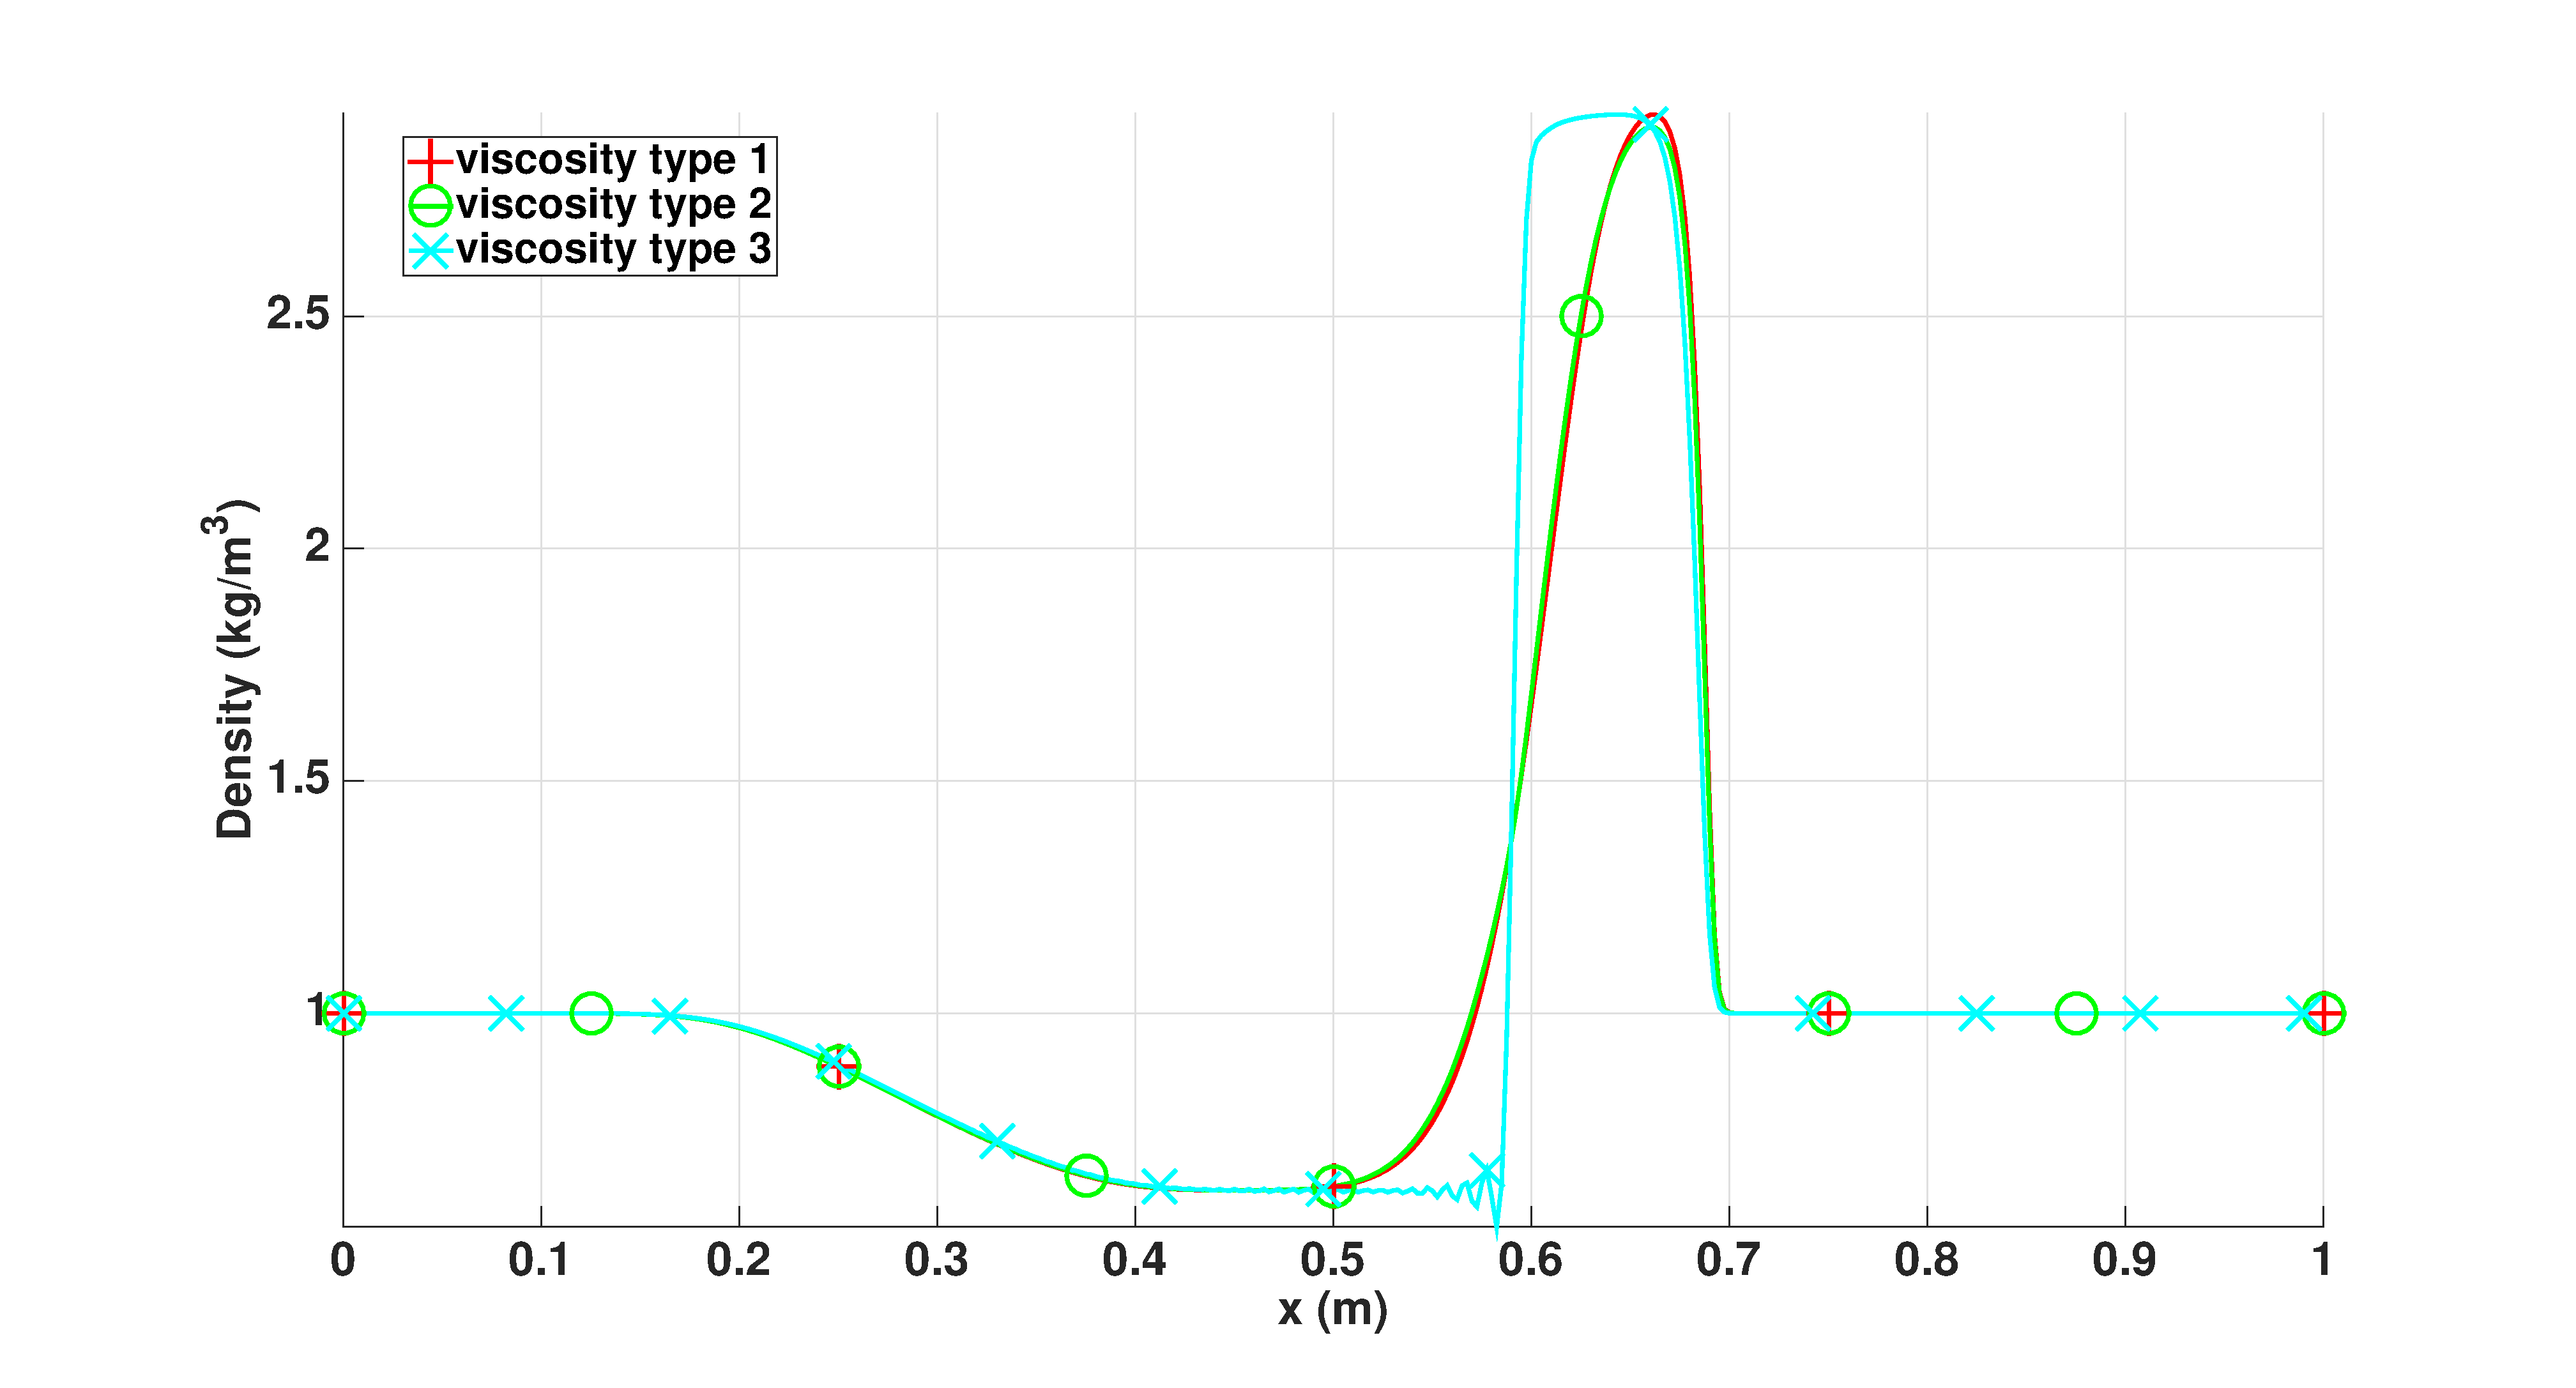
\includegraphics[width=\textwidth]{figures/relaxation_vapor_density_multiple_visc.eps}
                \caption{Liquid density}
                \label{fig:liq-density}
        \end{subfigure}
				\\
        \begin{subfigure}[b]{0.95\textwidth}
                \centering
                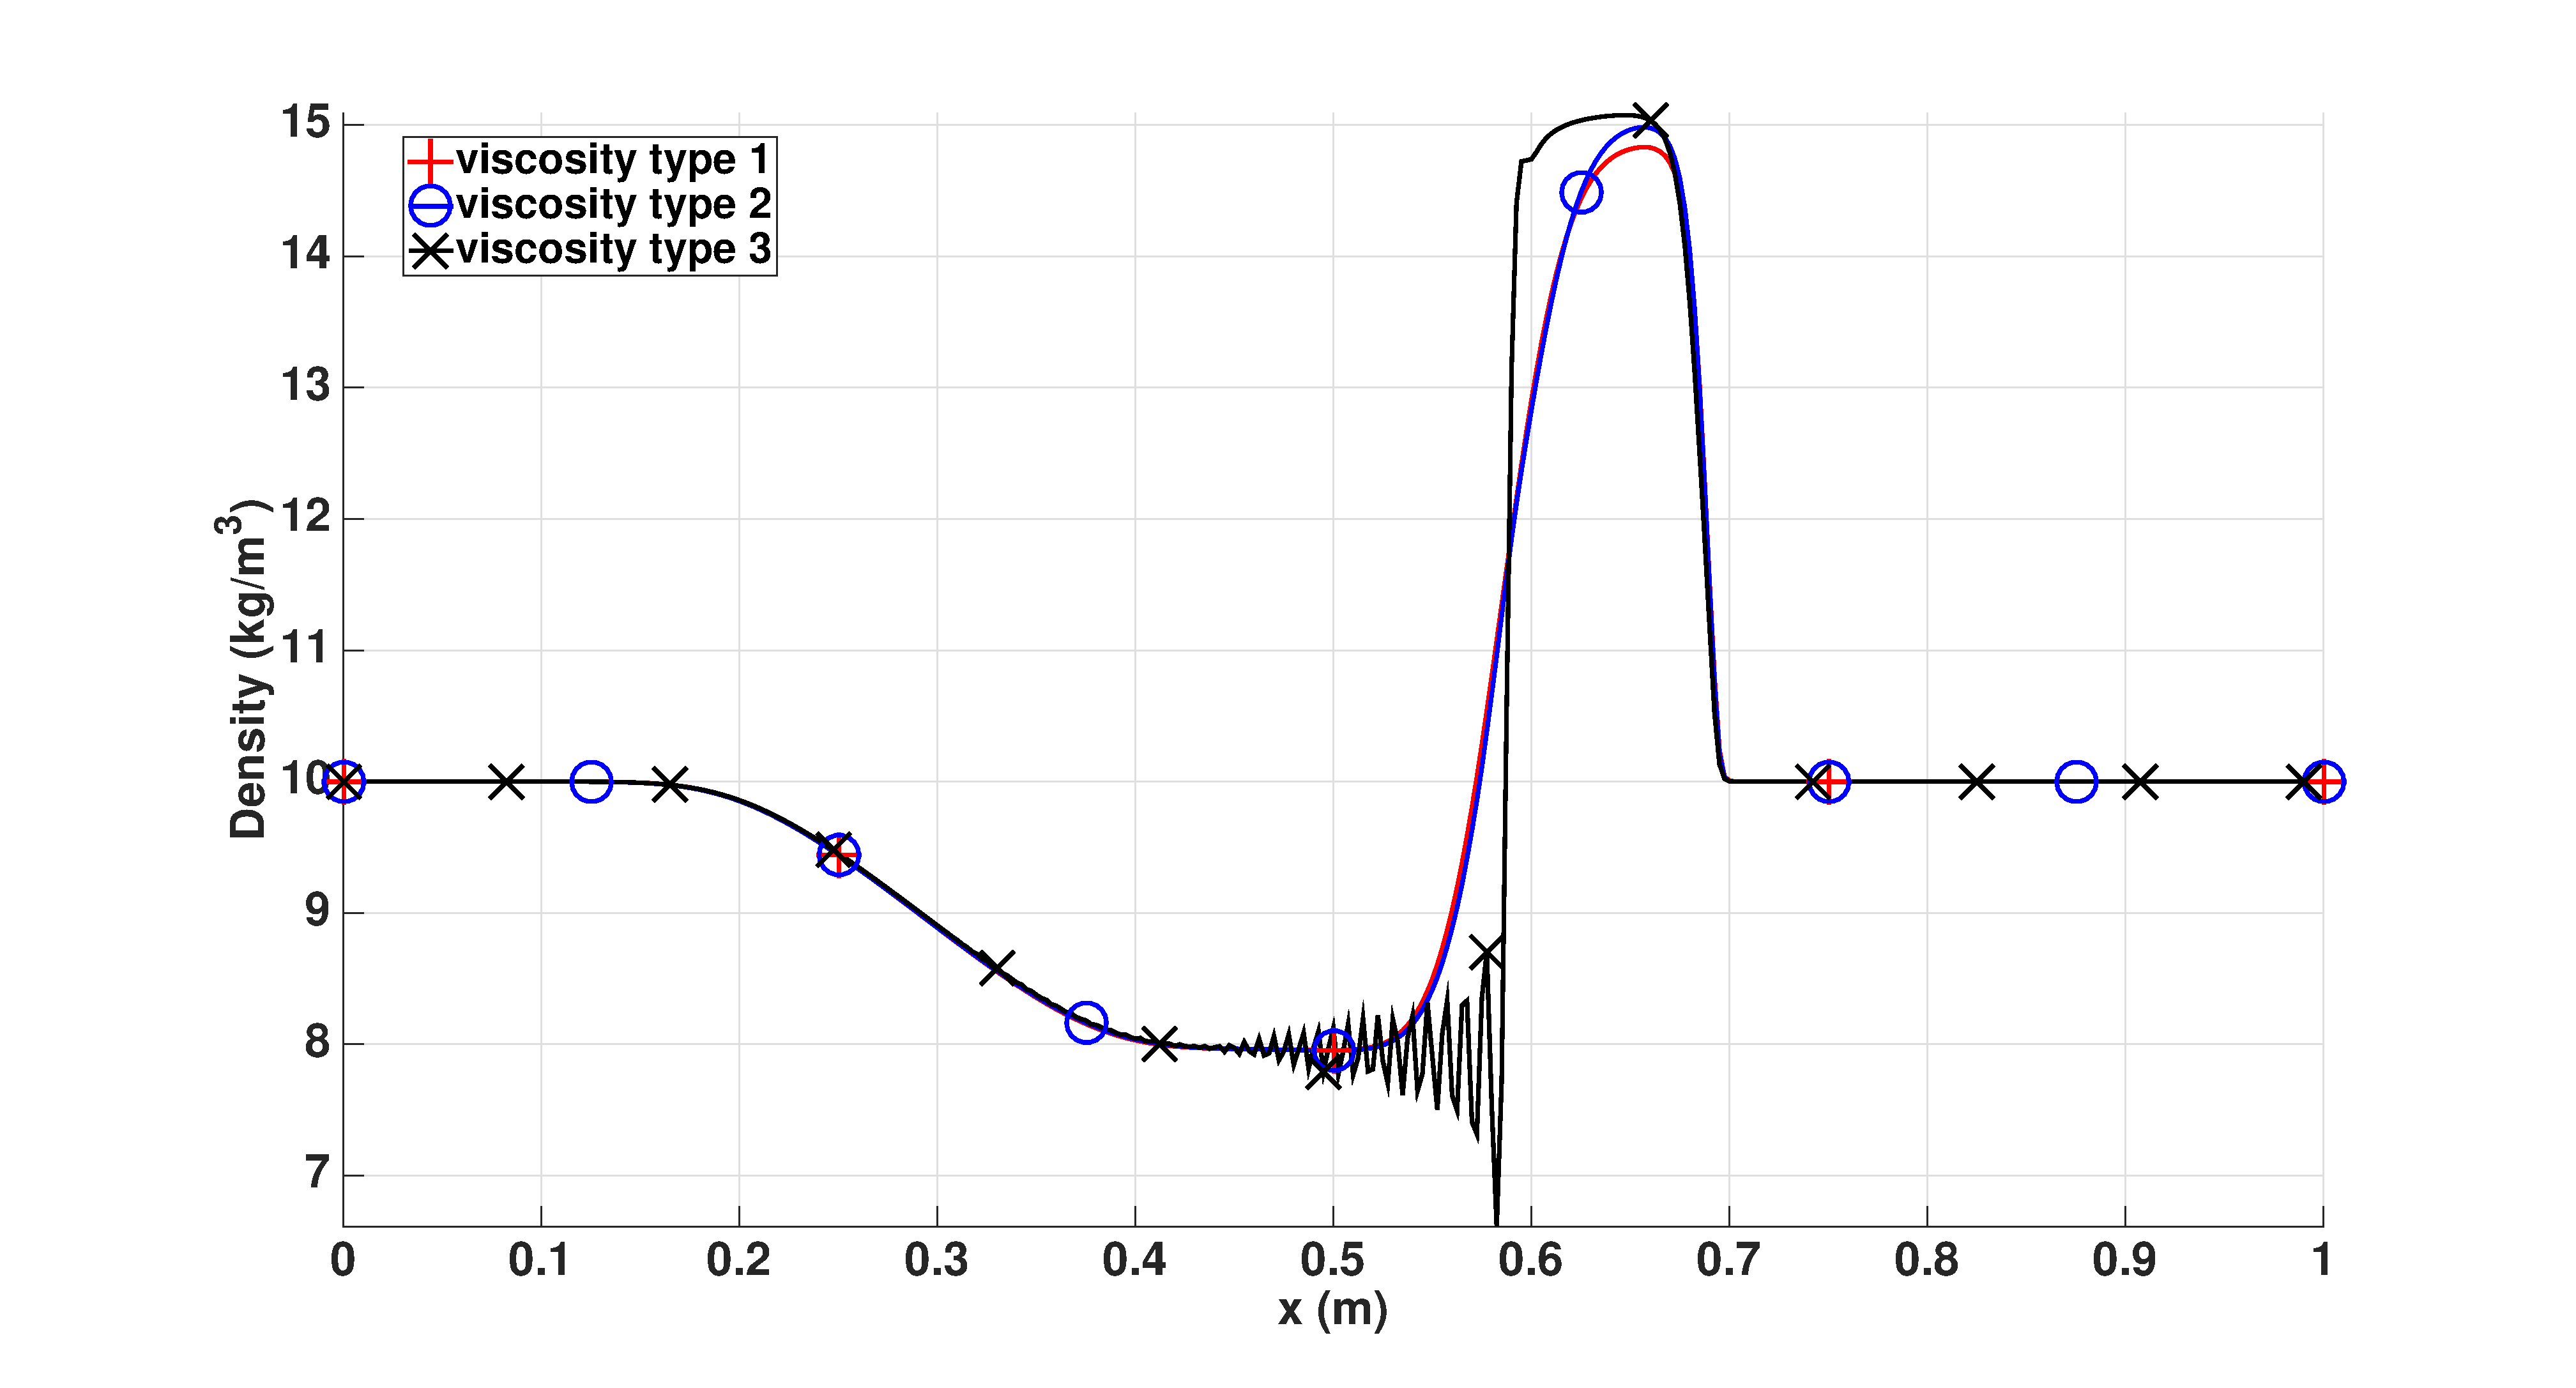
\includegraphics[width=\textwidth]{figures/relaxation_liquid_density_multiple_visc.eps}
                \caption{Vapor density}
                \label{fig:vap-density}
        \end{subfigure}
        \caption{Shock tube results: liquid and vapor densities computed using three different viscosity types at $t=473 \ \mu s$.}\label{fig:density}
\end{figure}
%
In cases (1) and (2), the numerical solutions do not display any instability in the density profiles. Case (3) displays oscillations, which is expected since the continuity equations are not regularized (similarly to the results obtained in the single-phase case, \cite{jlg_VR_SIAM_2004}).
%
\begin{figure}[H]
        \centering
        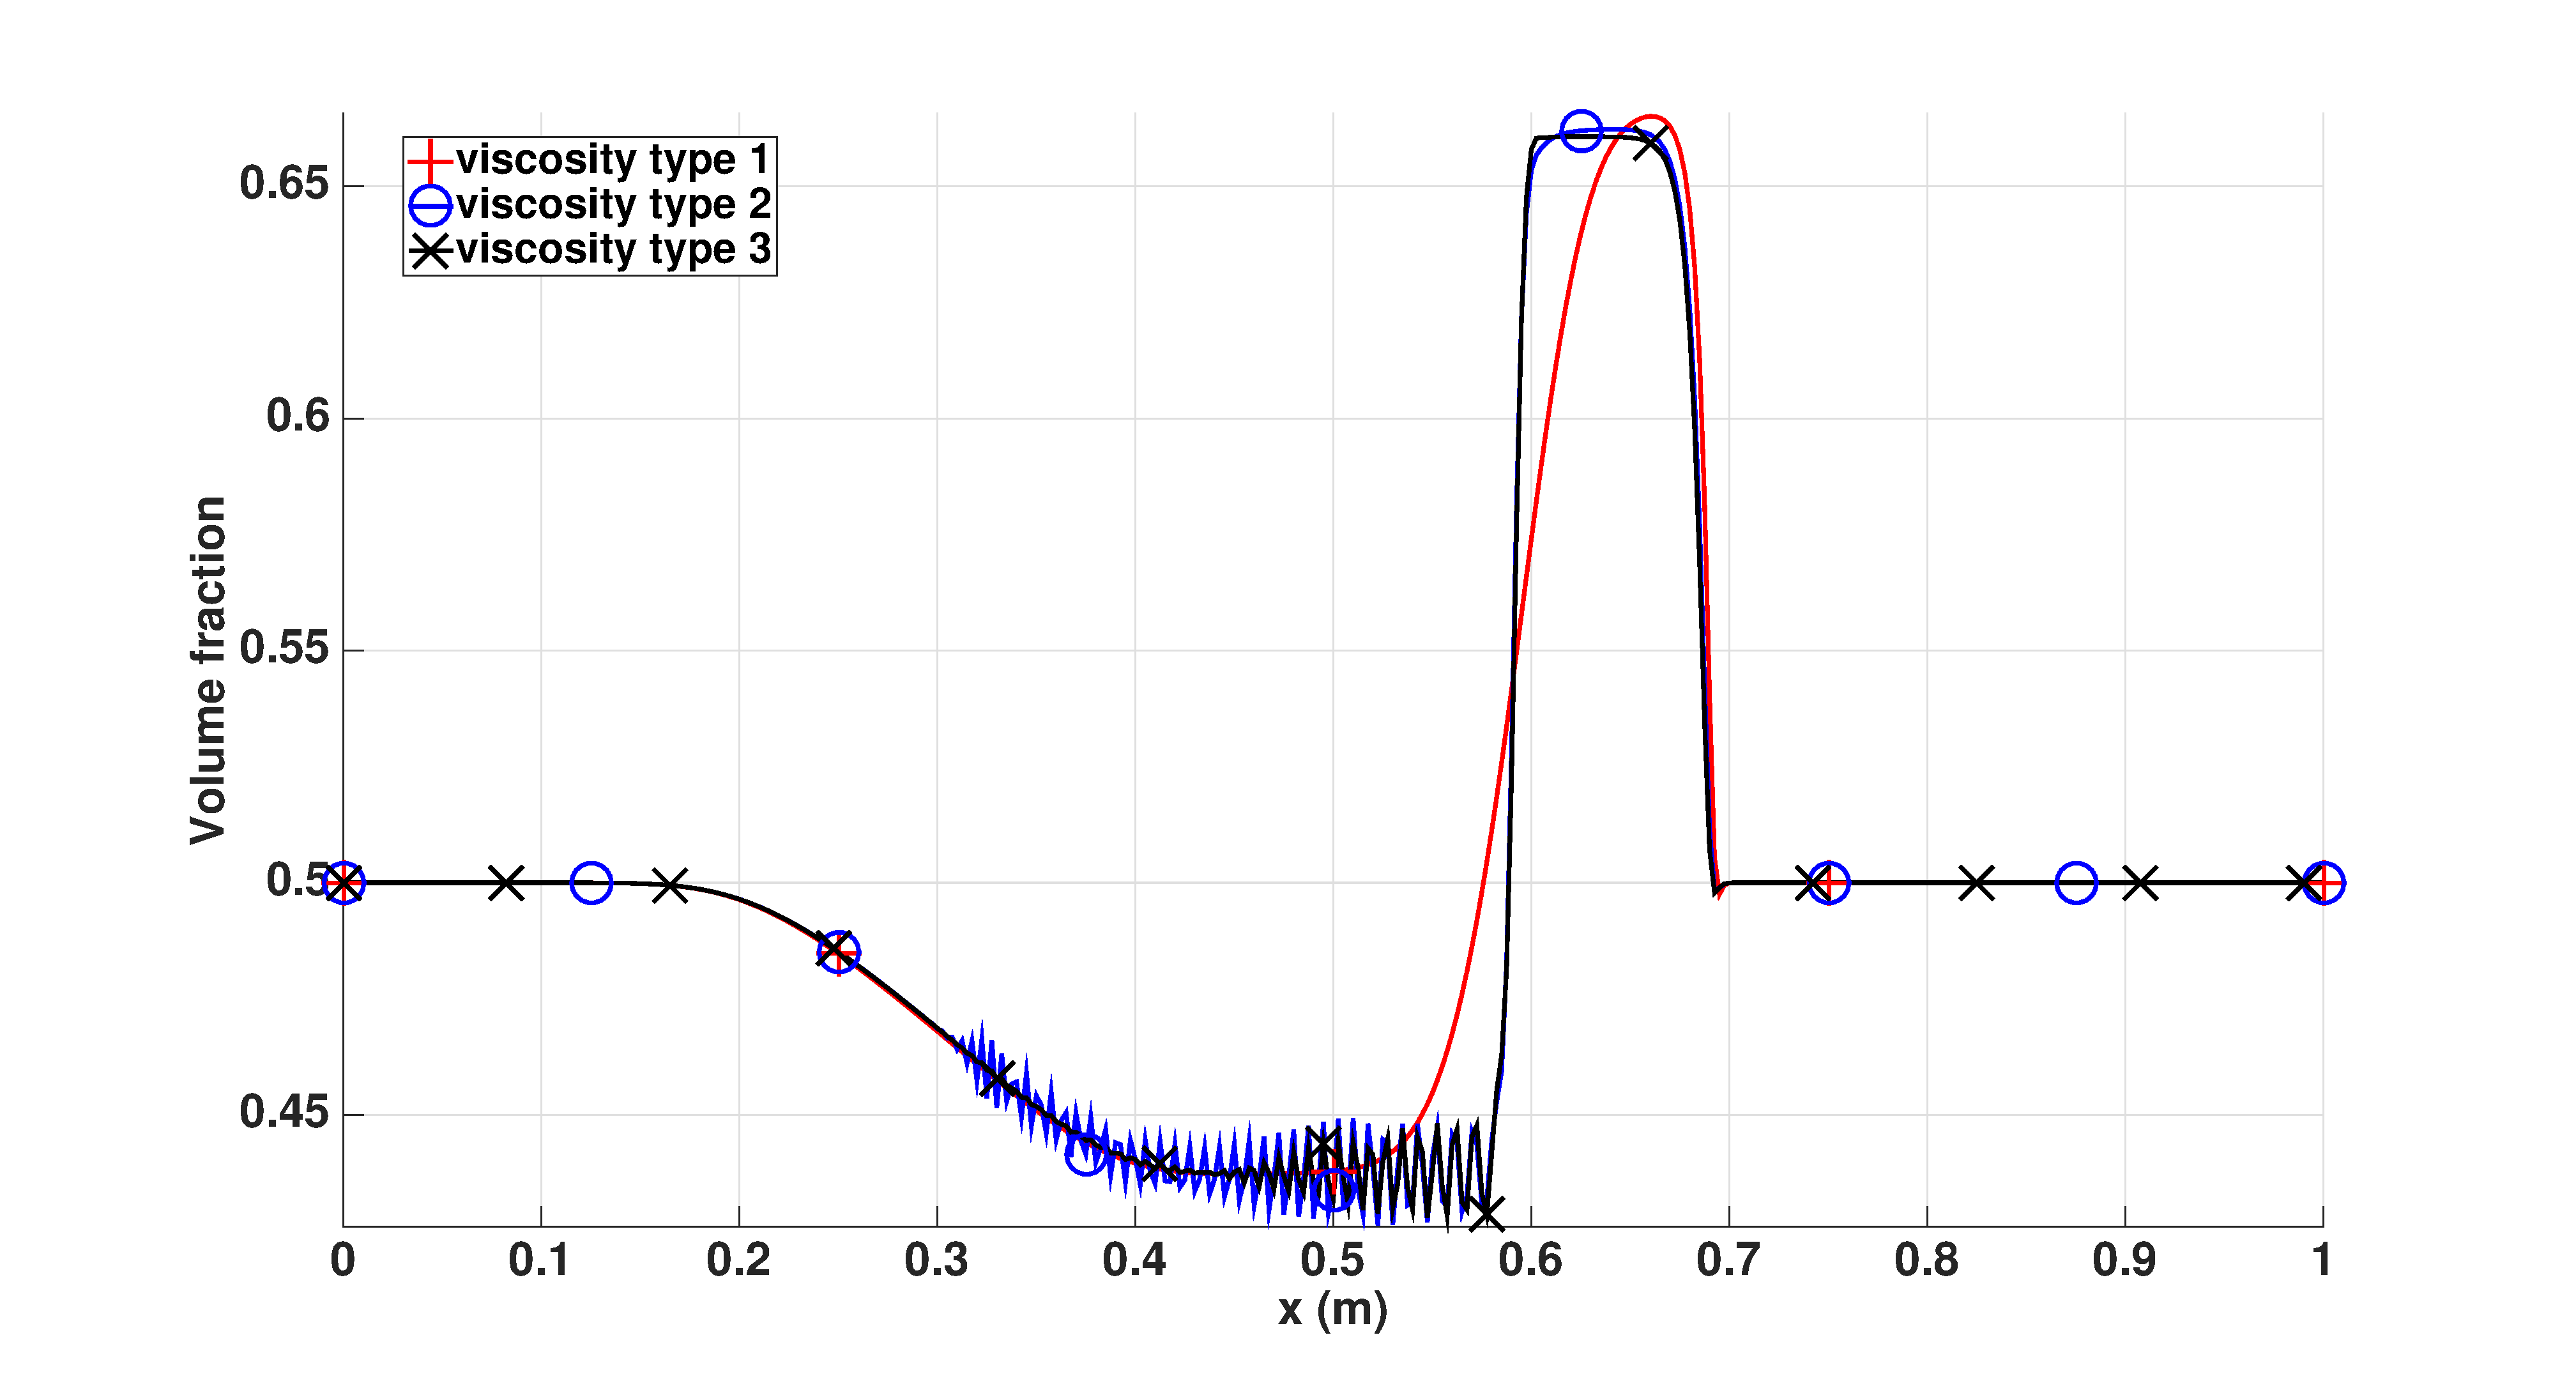
\includegraphics[width=\textwidth]{figures/relaxation_liquid_vf_multiple_visc.eps}
        \caption{Liquid volume fraction obtained using three different viscosity types at $t=473 \ \mu s$.}
        \label{fig:liq-vf}
\end{figure}
%
When inspecting the volume fraction profiles near the contact region (see \fig{fig:liq-vf}), one notices that as soon as $\beta_k=0$ 
(cases (2) and (3)), the simulations exhibit spurious oscillations in the contact region. 
In case (3), the continuity and the volume fraction equations are both no longer regularized ($\kappa_k=\beta_k=0$); this leads to 
the formation of instabilities in the pre-contact region, the presence of an undershoot in the density profile and an overshoot in the volume fraction profile in the post-contact region as shown in \fig{fig:density} and \fig{fig:liq-vf}, respectively. 

%This result is consistent with 
%the study performed by Guermond et al. in \cite{jlg_VR_SIAM_2004} for single-phase Euler equations where they compared numerical solutions obtained using 
%a parabolic regularization (which included a dissipative term in the continuity equation) and with numerical solutions obtained using a 
%Navier-Stokes regularization (no artificial viscosity terms in the continuity equation).
%
%----------------------------------------------------------
\subsection{Multi-Mach mixture flow test case}\label{sec:second-test}
%-----------------------------------------------------------
%
To illustrate the low-Mach asymptotic study presented in \sct{sec:low-Mach}, a 1-D converging-diverging nozzle problem is considered 
for a two-phase flow where the relaxation coefficients $\mu_P$ and $\lambda_u$ are set to zero (independent phases).
%
The variable area expression for the nozzle is given by $A(x) = 1 + \tfrac{1}{2} \cos(2 \pi x / L)$ with length $L=1\ m$. 
At the inlet, the stagnation pressure and temperature are set to $P_0 = 1$ {\it MPa} and $T_0 = 453\ K$, respectively. 
At the outlet, only the static pressure is specified: $P_s = 0.5$ {\it MPa}. 
Initially, the two phases are at rest; their temperatures are uniform and equal to their stagnation temperatures;  their pressures 
linearly decrease from the stagnation pressure inlet value to the static pressure outlet value. The volume fraction $\alpha_k$ is set to $0.5$.
The stiffened gas equation of state, \eqt{eq:sgeos}, is used to model the liquid and vapor with the parameters provided in \tbl{tbl:stff_gas_eos}.
%
\begin{table}[!htbp]
\begin{center}
\caption{ Stiffened Gas Equation of State parameters for steam and liquid water.}
\label{tbl:stff_gas_eos}
\begin{tabular}{|c|c|c|c|c|}
 \hline
\text{fluid}      & $\gamma_k$ & $C_{v,k}$ $(J.kg^{-1}.K^{-1})$ & $P_{\infty,k}$ $(Pa)$ & $q_k$ $(J.kg^{-1})$ \\  \hline \hline
liquid & 2.35     & 1816     & $10^9$                    & $-1167\ 10^3$                          \\  \hline
vapor  & 1.43     & 1040     & 0                         & $ 2030\ 10^3$                          \\  \hline
\end{tabular}
\end{center}
\end{table}
%
This test case is of interest for multiple reasons: (a) a steady state is reached, (b) 
an analytical solution is available \cite{nozzle_exact2,SEM}, (c) due to the different compressibilities between the phases,
the vapor phase will become supersonic and will develop a steady shock while the liquid phase will simultaneously be low-Mach flow ($M_\text{liquid} \approx 10^{-2}$). 
%
We illustrate the low-Mach asymptotic study of \sct{sec:low-Mach} with two cases. 
%
In case (1), the nozzle problem is run using the same phasic viscosity 
coefficients that were used for the previous shock tube test case (\sct{sec:first-test}), i.e., 
$\mu_k =  \kappa_k = \beta_k = \tfrac{h}{2} \left( ||\mbold u_k|| + c_k \right)$ 
(note that the dissipative term in the volume fraction is not active because the volume fraction remains constant here). 
Using these definitions for the viscosity coefficients in the the expressions for the Reynolds and P\'eclet numbers, \eqt{eq:ref_numb}, 
we obtain: $\Re_k=\Pe_k^\kappa=\Pe_k^\beta = 2M_k / (1+M_k)$. 
% (note that the P\'eclet numbers defined for the volume fraction equation is not defined since the volume fraction equation is not needed). 
Such a scaling will efficiently stabilize the vapor flow that becomes supersonic in the nozzle ($M_k \sim 1 $). On the other hand, the liquid phase will reach 
a low-Mach steady-state flow and the above definitions of the viscosity coefficients are ill-scaled because they lead to $\Re_k=\Pe_k^\kappa=\Pe_k^\beta \propto M_k$ 
while the low-Mach asymptotic analysis of \sct{sec:low-Mach-sem} requires that these non-dimensionalized numbers scale as 1 in the low-Mach regime (i.e., the local Lax-Friedrichs viscosities are too large in the low-Mach regime). Hence, the correct steady-state solution
should not be obtained for the liquid phase using these viscosity definitions. 
%
In case (2), we propose a fix to the ill-scaling effects observed in the liquid phase by having non-dimensionalized numbers scaling as 1
for low-Mach flows. Hence, the following definitions of the phasic viscosity are used:  $\mu_k =  \kappa_k = \beta_k = M_k \times \tfrac{h}{2} \left( ||\mbold u_k|| + c_k \right)$. 
Now, in the low-Mach regime, we have $\Re_k$, $\Pe_k^\kappa$, and $=\Pe_k^\beta$ scaling as 1. Note that in the supersonic case, the 
viscous stabilization of the scheme is not altered since $M_k \simeq \mathcal{O}(1)$. 

The steady-state numerical solutions for liquid and vapor phases are presented in \fig{fig:vap-phase} and \fig{fig:liq-phase}, respectively, 
for the above cases (1) and (2). 

%
\begin{figure}[H]
        \centering
        \begin{subfigure}[b]{0.5\textwidth}
                \centering
                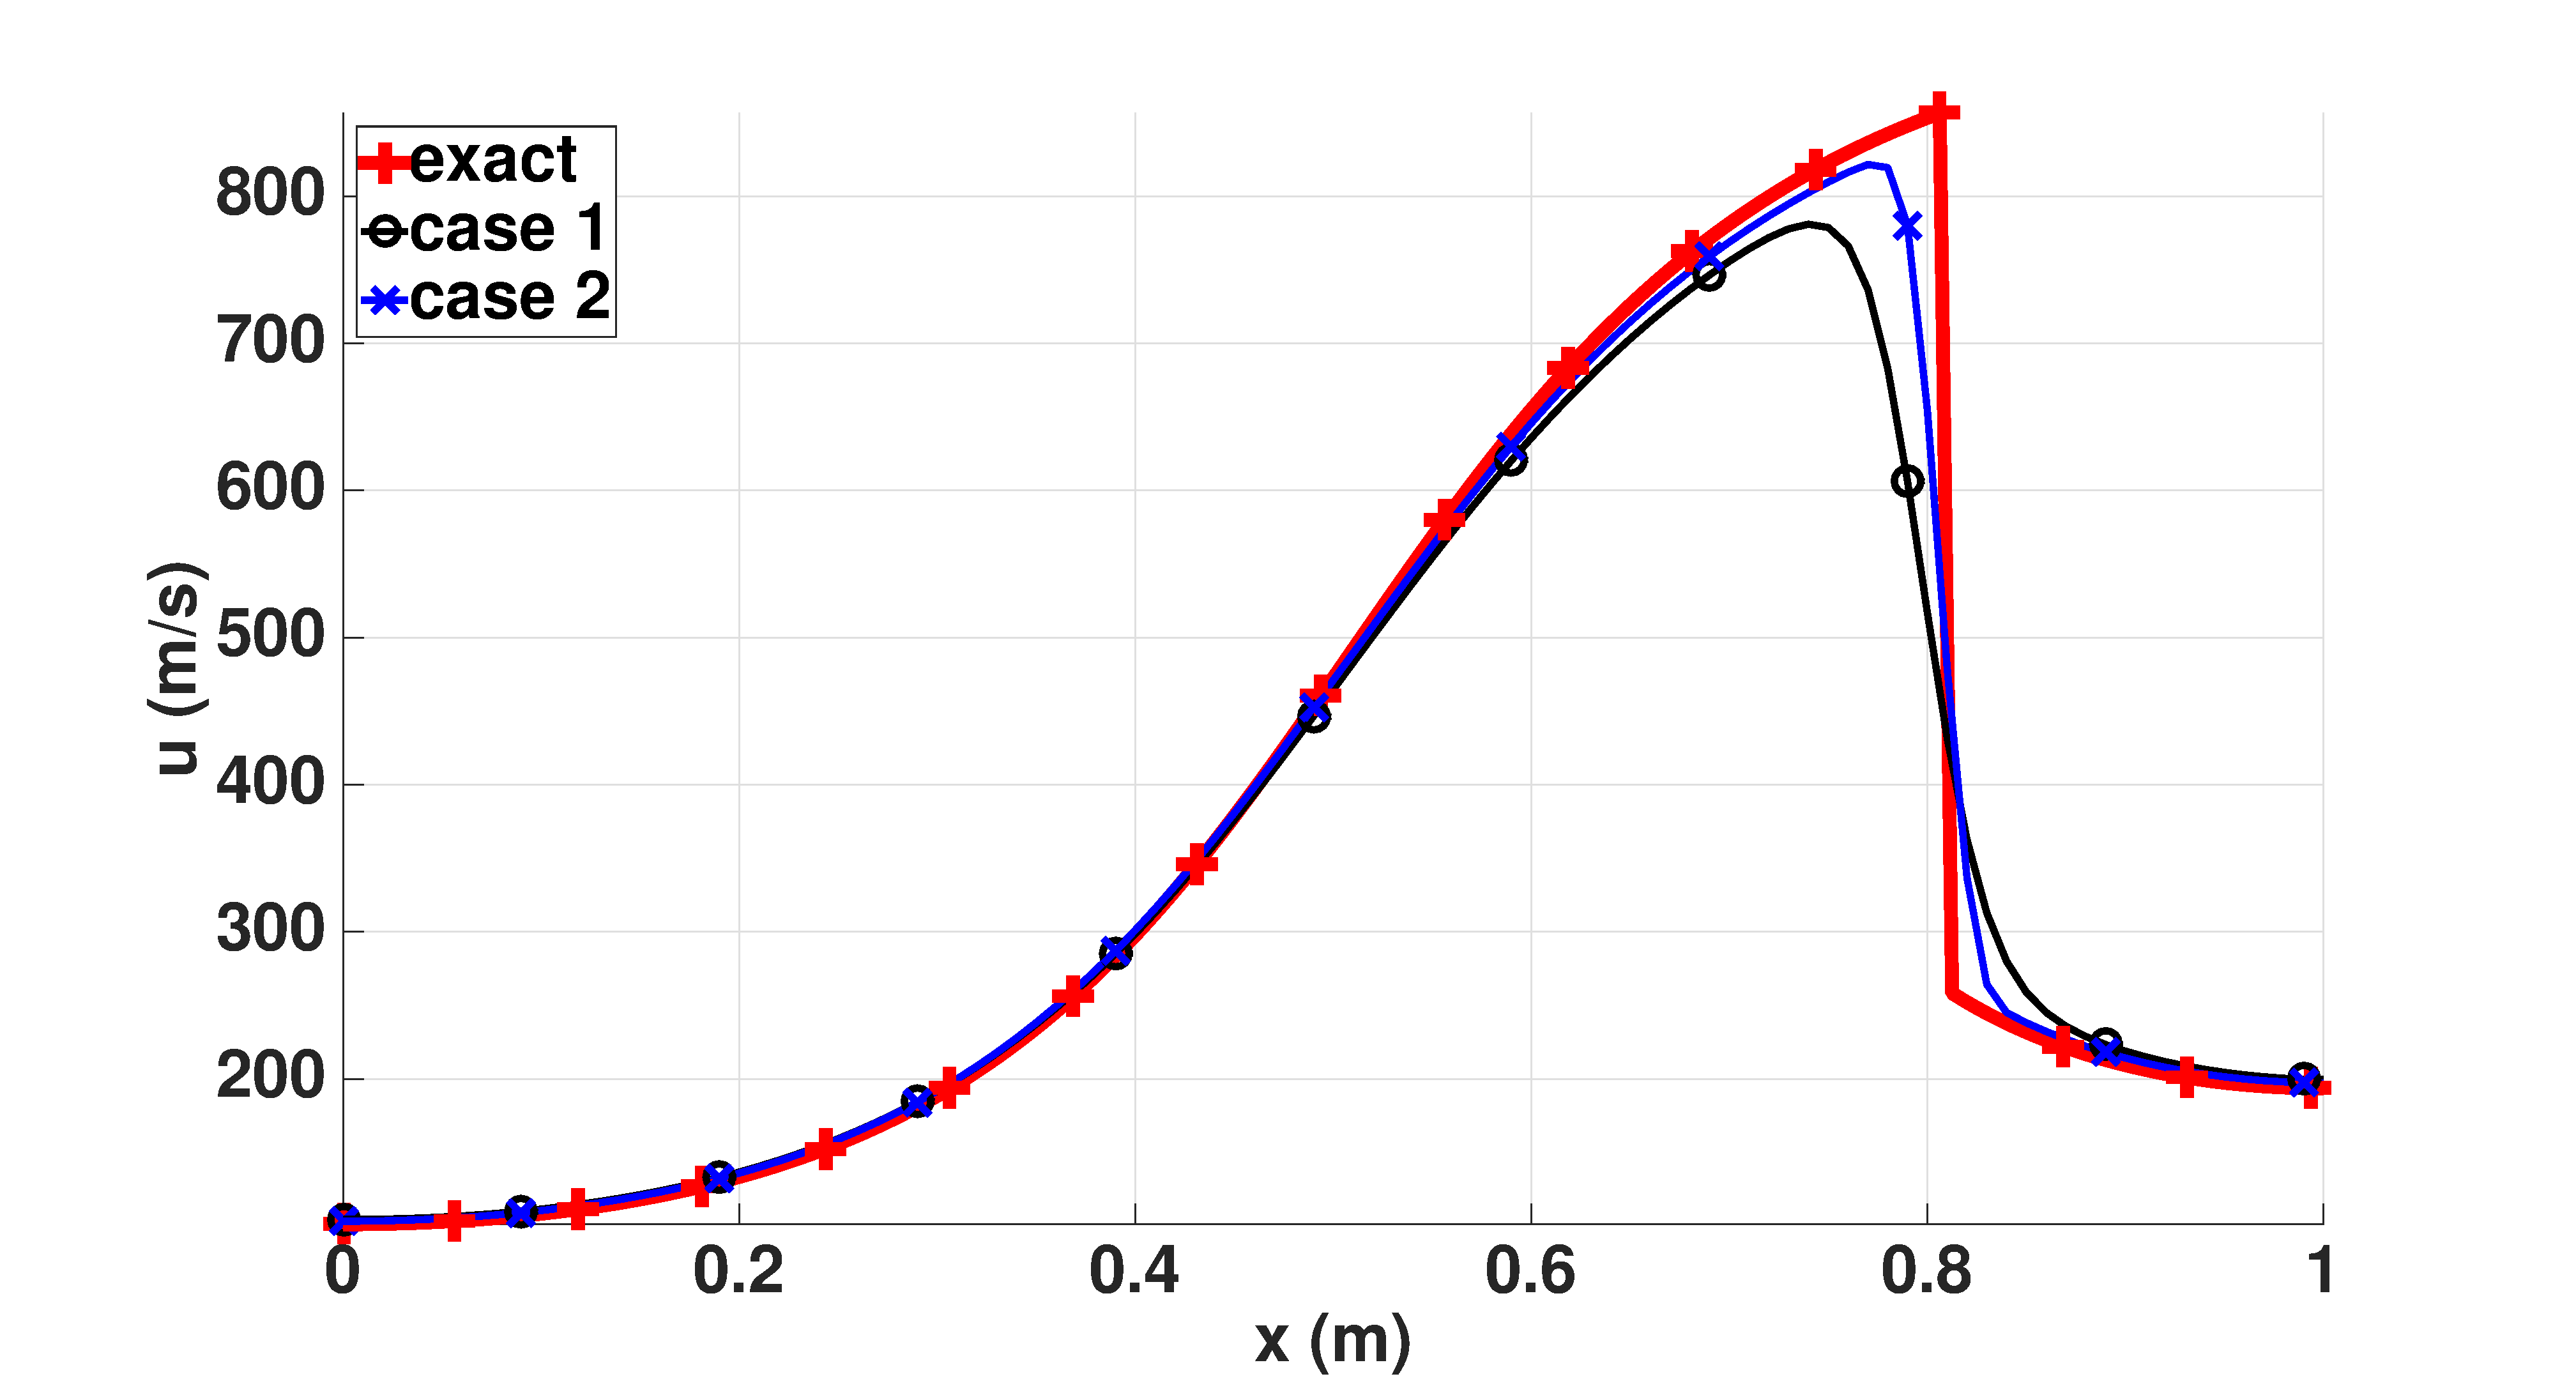
\includegraphics[width=\textwidth]{figures/vapor_velocity_llf_and_exact_100.eps}
                \caption{Velocity}
                \label{fig:vap-phase-vel}
        \end{subfigure}%
        \begin{subfigure}[b]{0.5\textwidth}
                \centering
                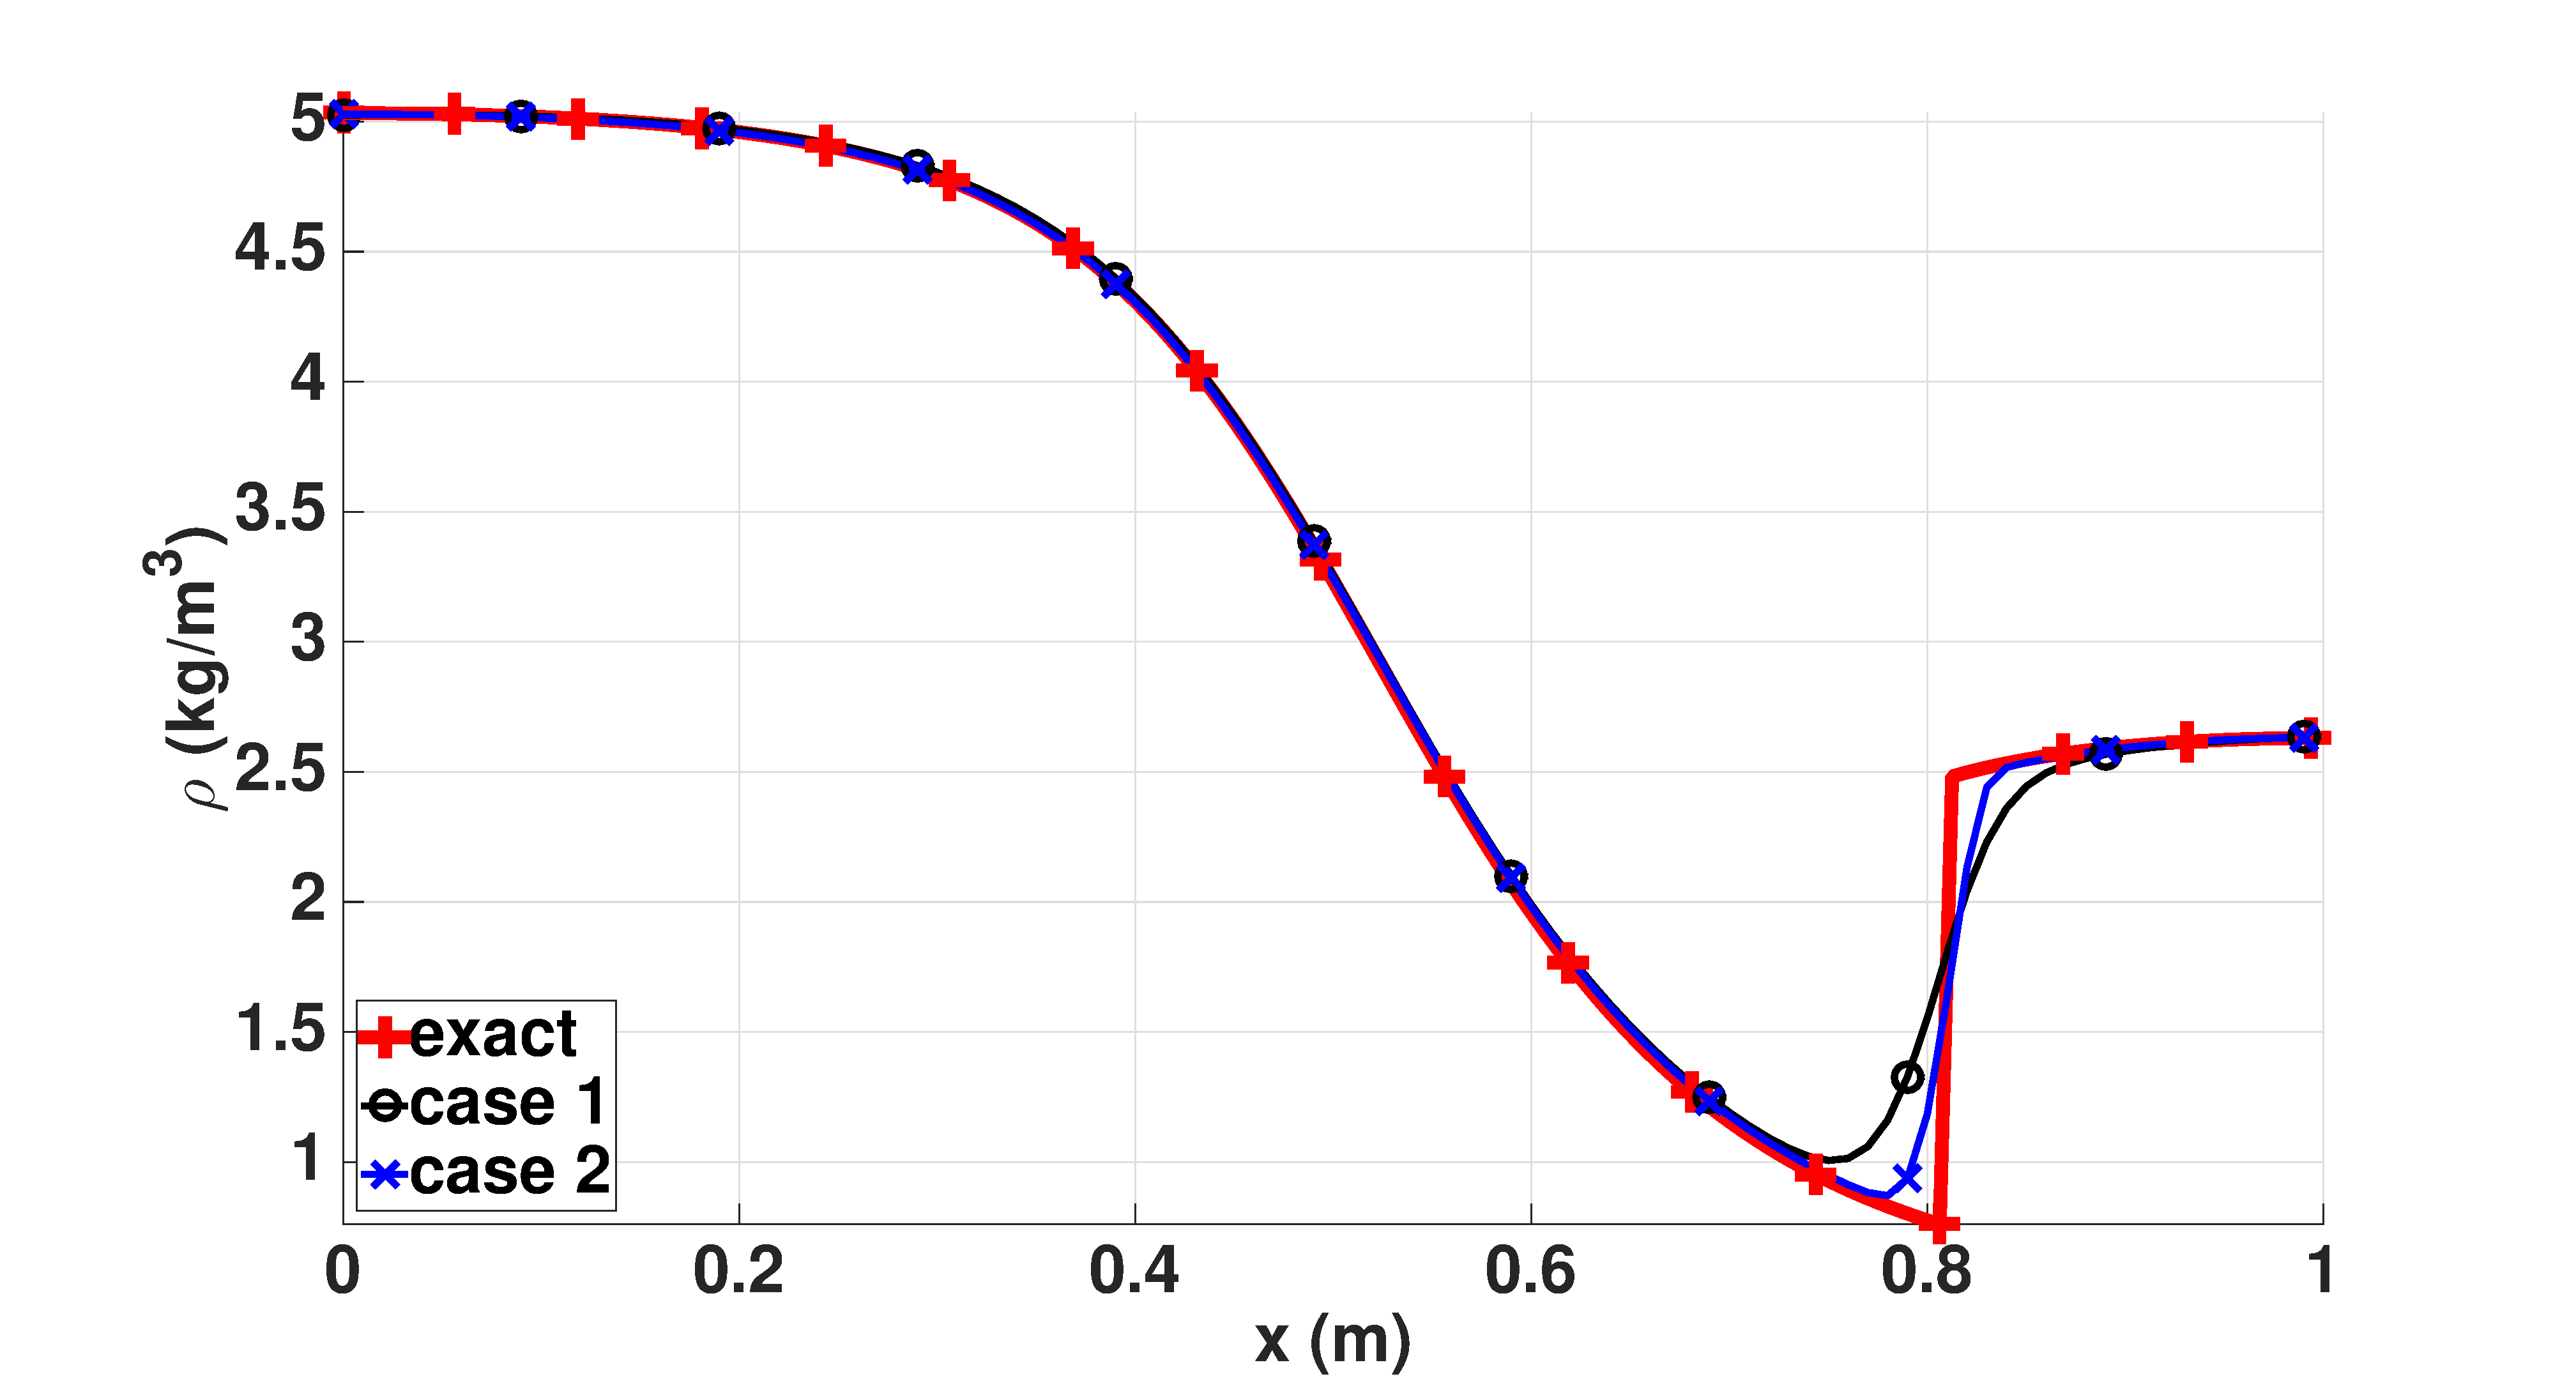
\includegraphics[width=\textwidth]{figures/vapor_density_llf_and_exact_100.eps}
                \caption{Density}
                \label{fig:vap-phase-density}
        \end{subfigure}
        
        \begin{subfigure}[b]{0.495\textwidth}
                \centering
                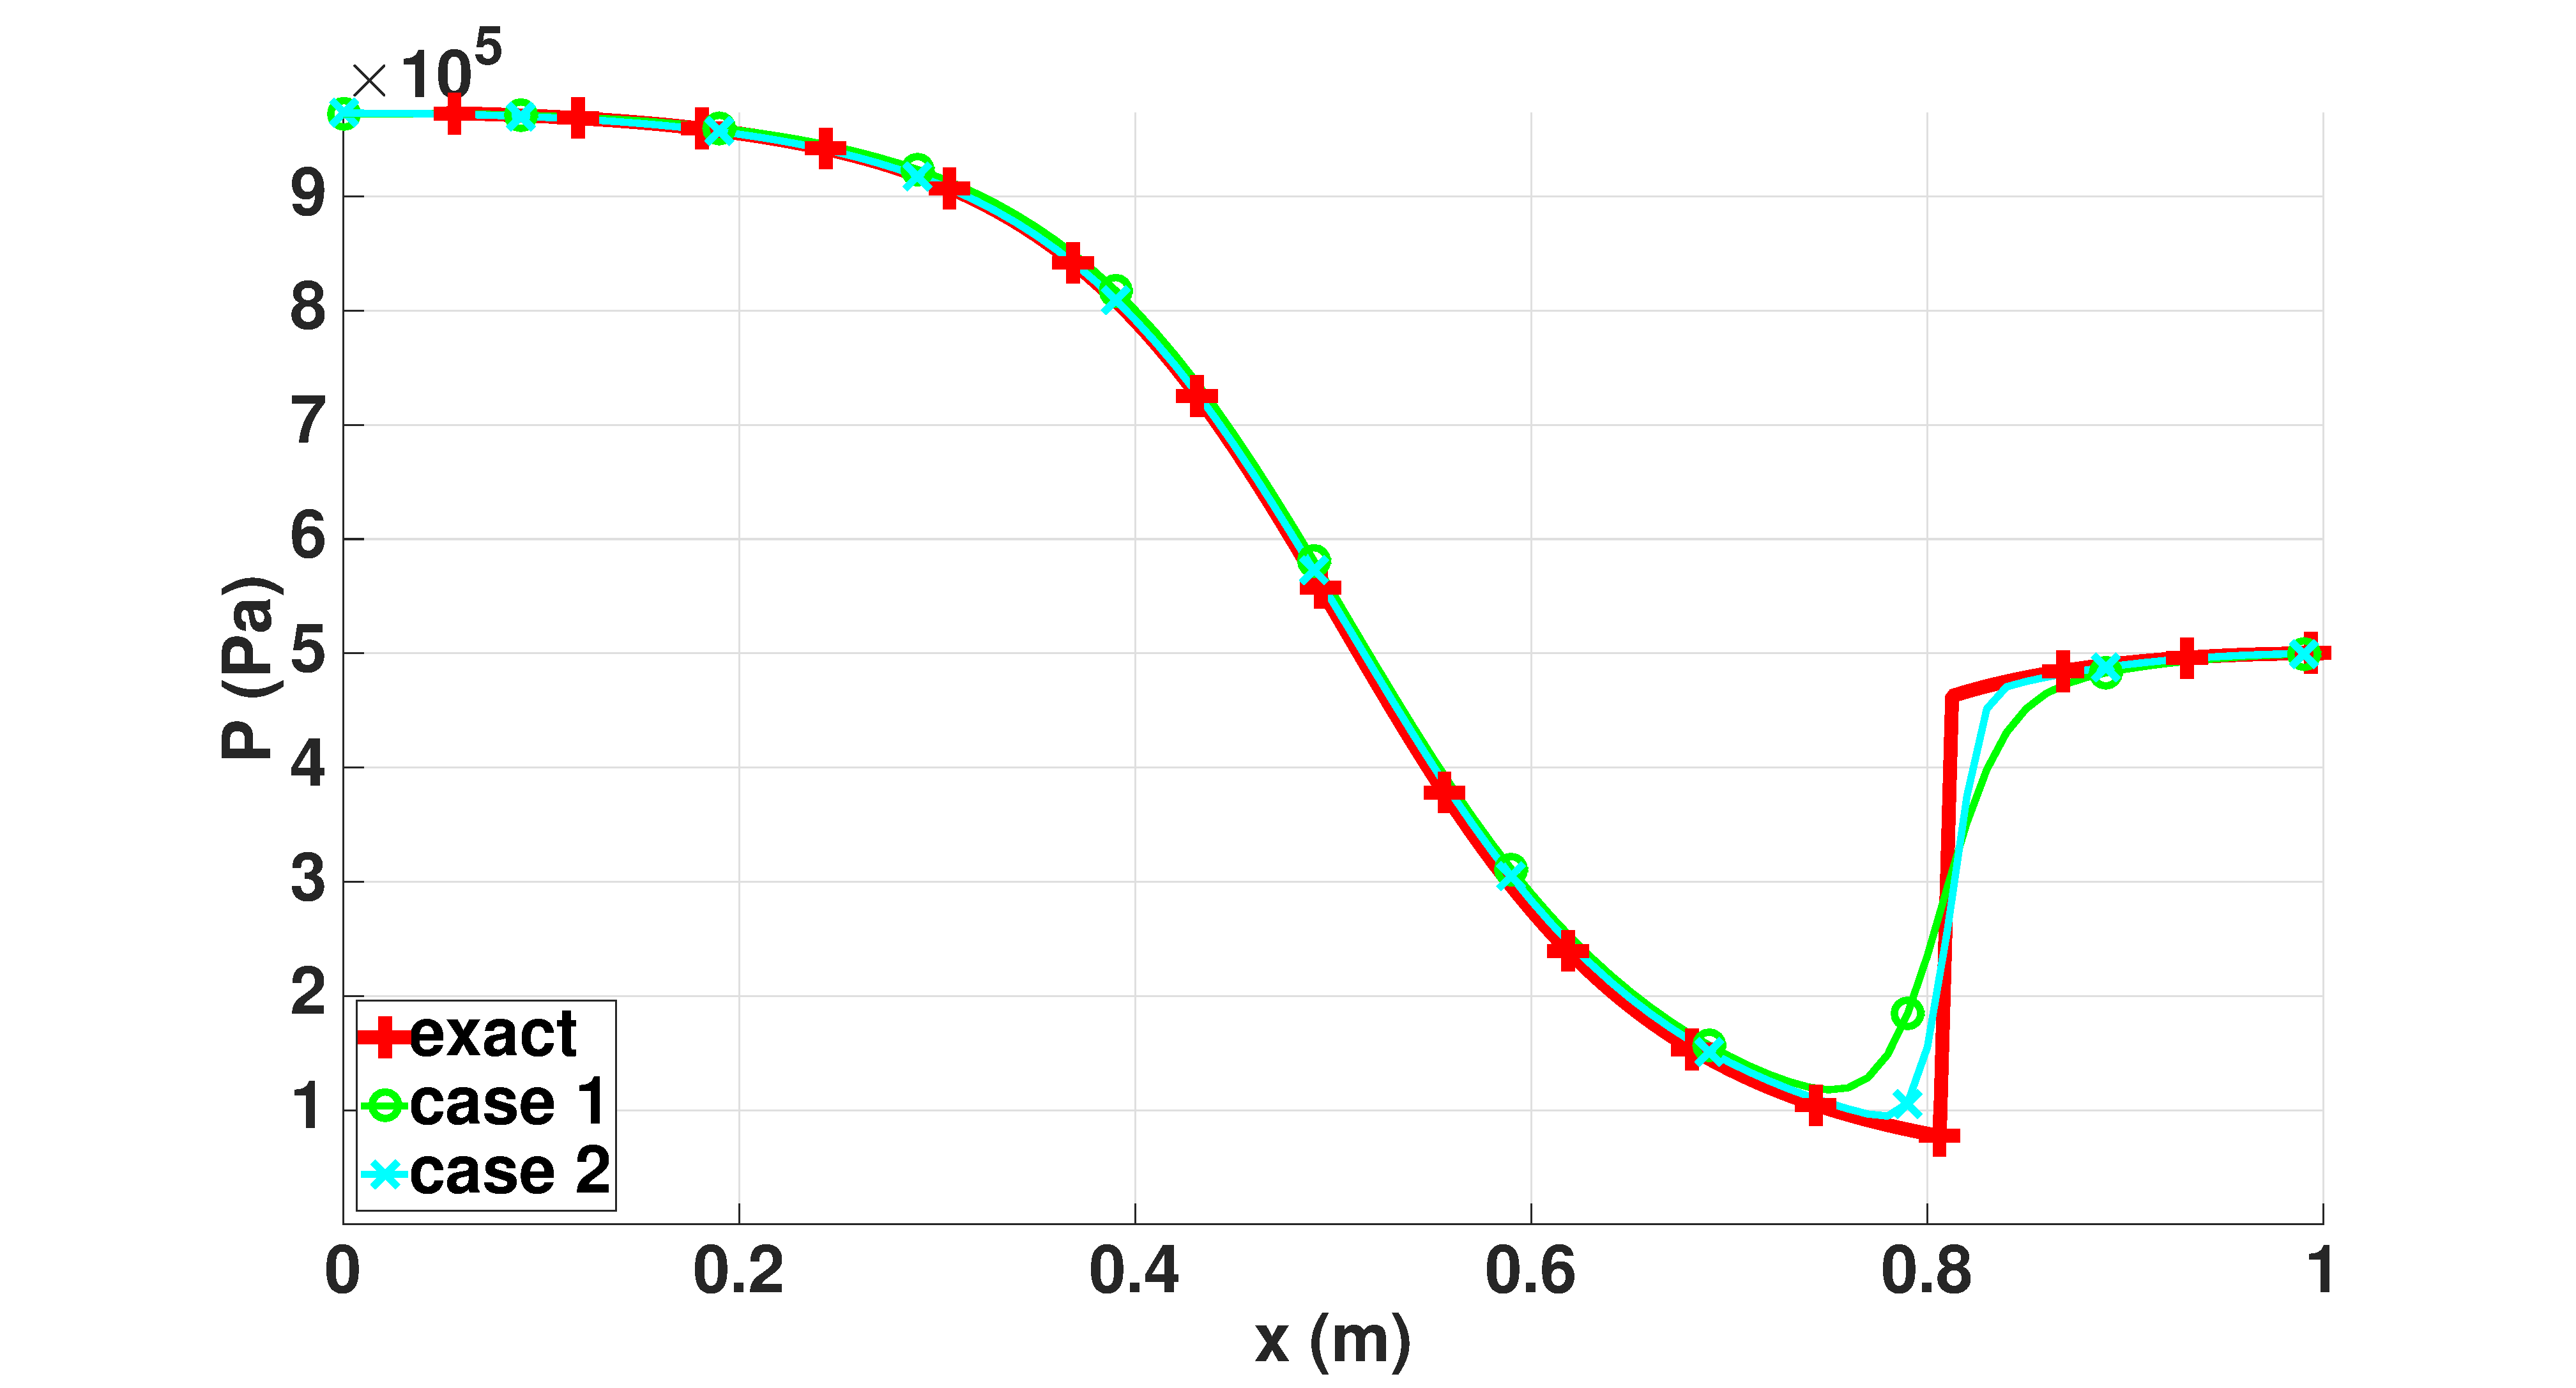
\includegraphics[width=\textwidth]{figures/vapor_pressure_llf_and_exact_100.eps}
                \caption{Pressure}
                \label{fig:vap-phase-press}
        \end{subfigure}        
        \begin{subfigure}[b]{0.495\textwidth}
                \centering
                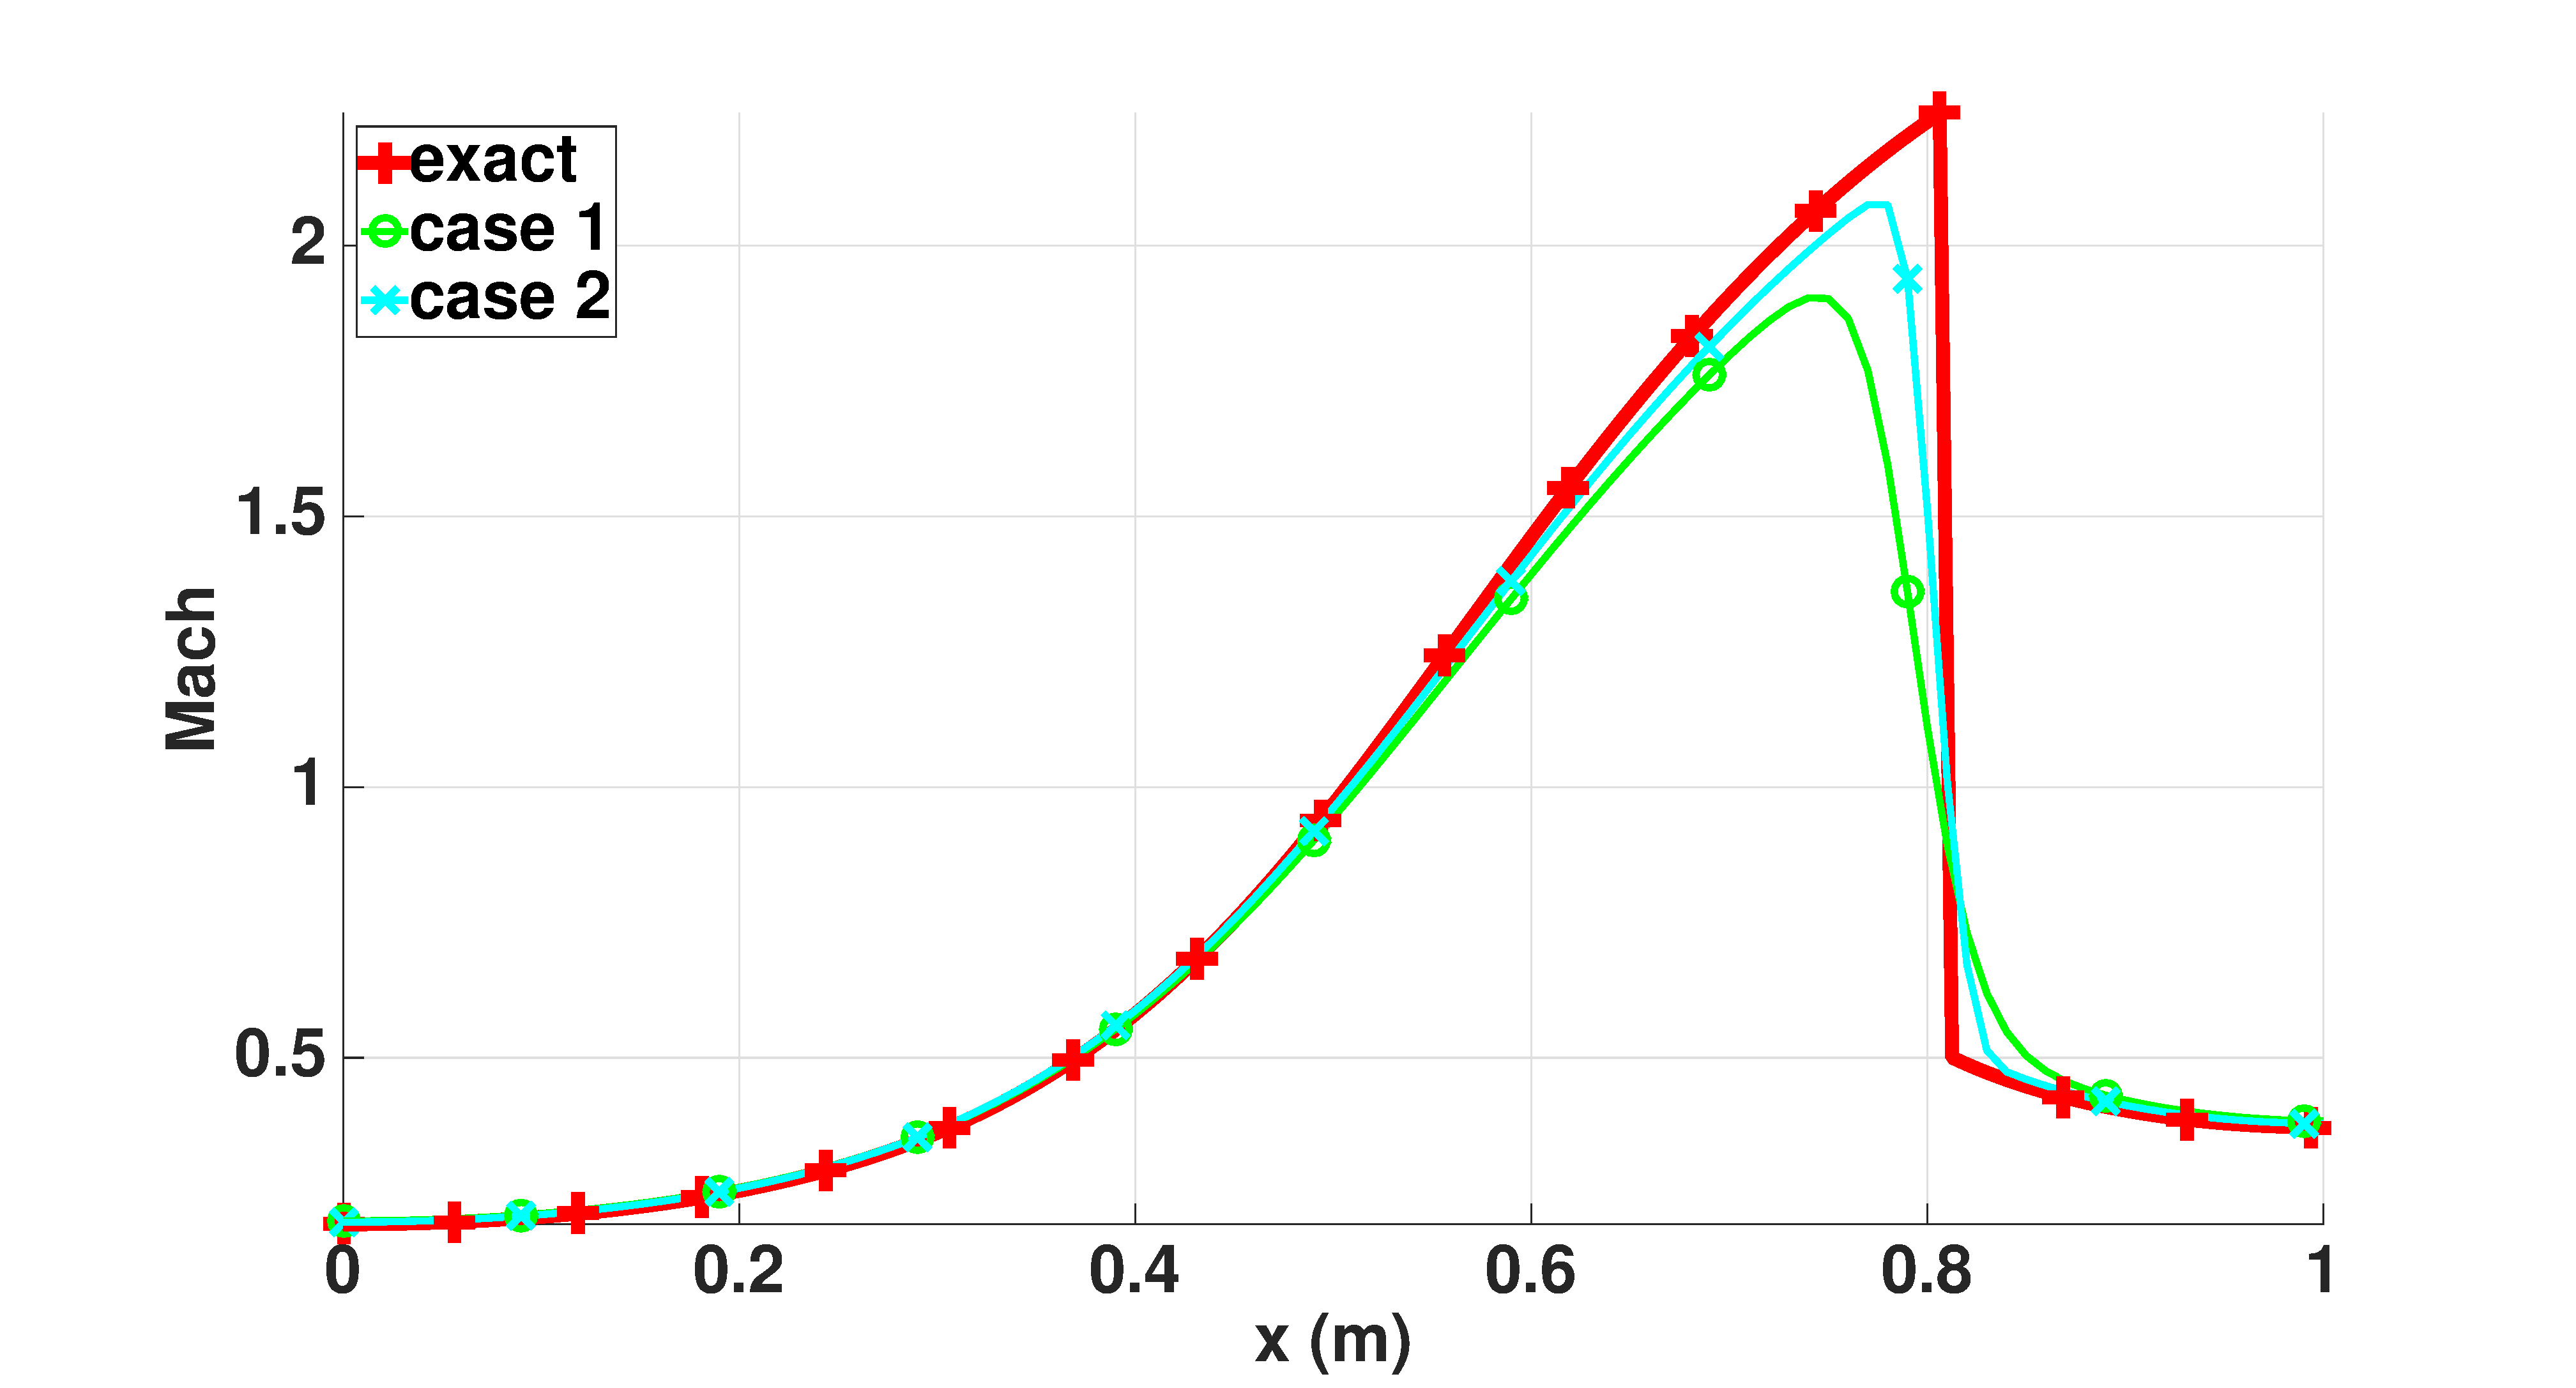
\includegraphics[width=\textwidth]{figures/vapor_mach_llf_and_exact_100.eps}
                \caption{Mach number}
                \label{fig:vap-phase-mach}
        \end{subfigure}
        \caption{Numerical and analytical steady-state vapor-phase solutions for the divergent-convergent two-phase flow nozzle problem.}\label{fig:vap-phase}
\end{figure}
%
In \fig{fig:vap-phase}, the numerical solutions obtained for the vapor phase in cases (1) and (2) are almost identical, as expected, because the Mach number is of order 1
(see Mach plot in \fig{fig:vap-phase-mach}). The numerical and exact solutions match  well, except in the vicinity of the shock where smoothing occurs due to the over-dissipative nature of the local Lax-Friedrichs viscosity. As the mesh is refined, it is observed (not shown) that the numerical solution converges to the exact solution. %, experiencing the same behavior as in \sct{sec:grid-conv-study}.
%
\begin{figure}[H]
        \centering
        \begin{subfigure}[b]{0.5\textwidth}
                \centering
                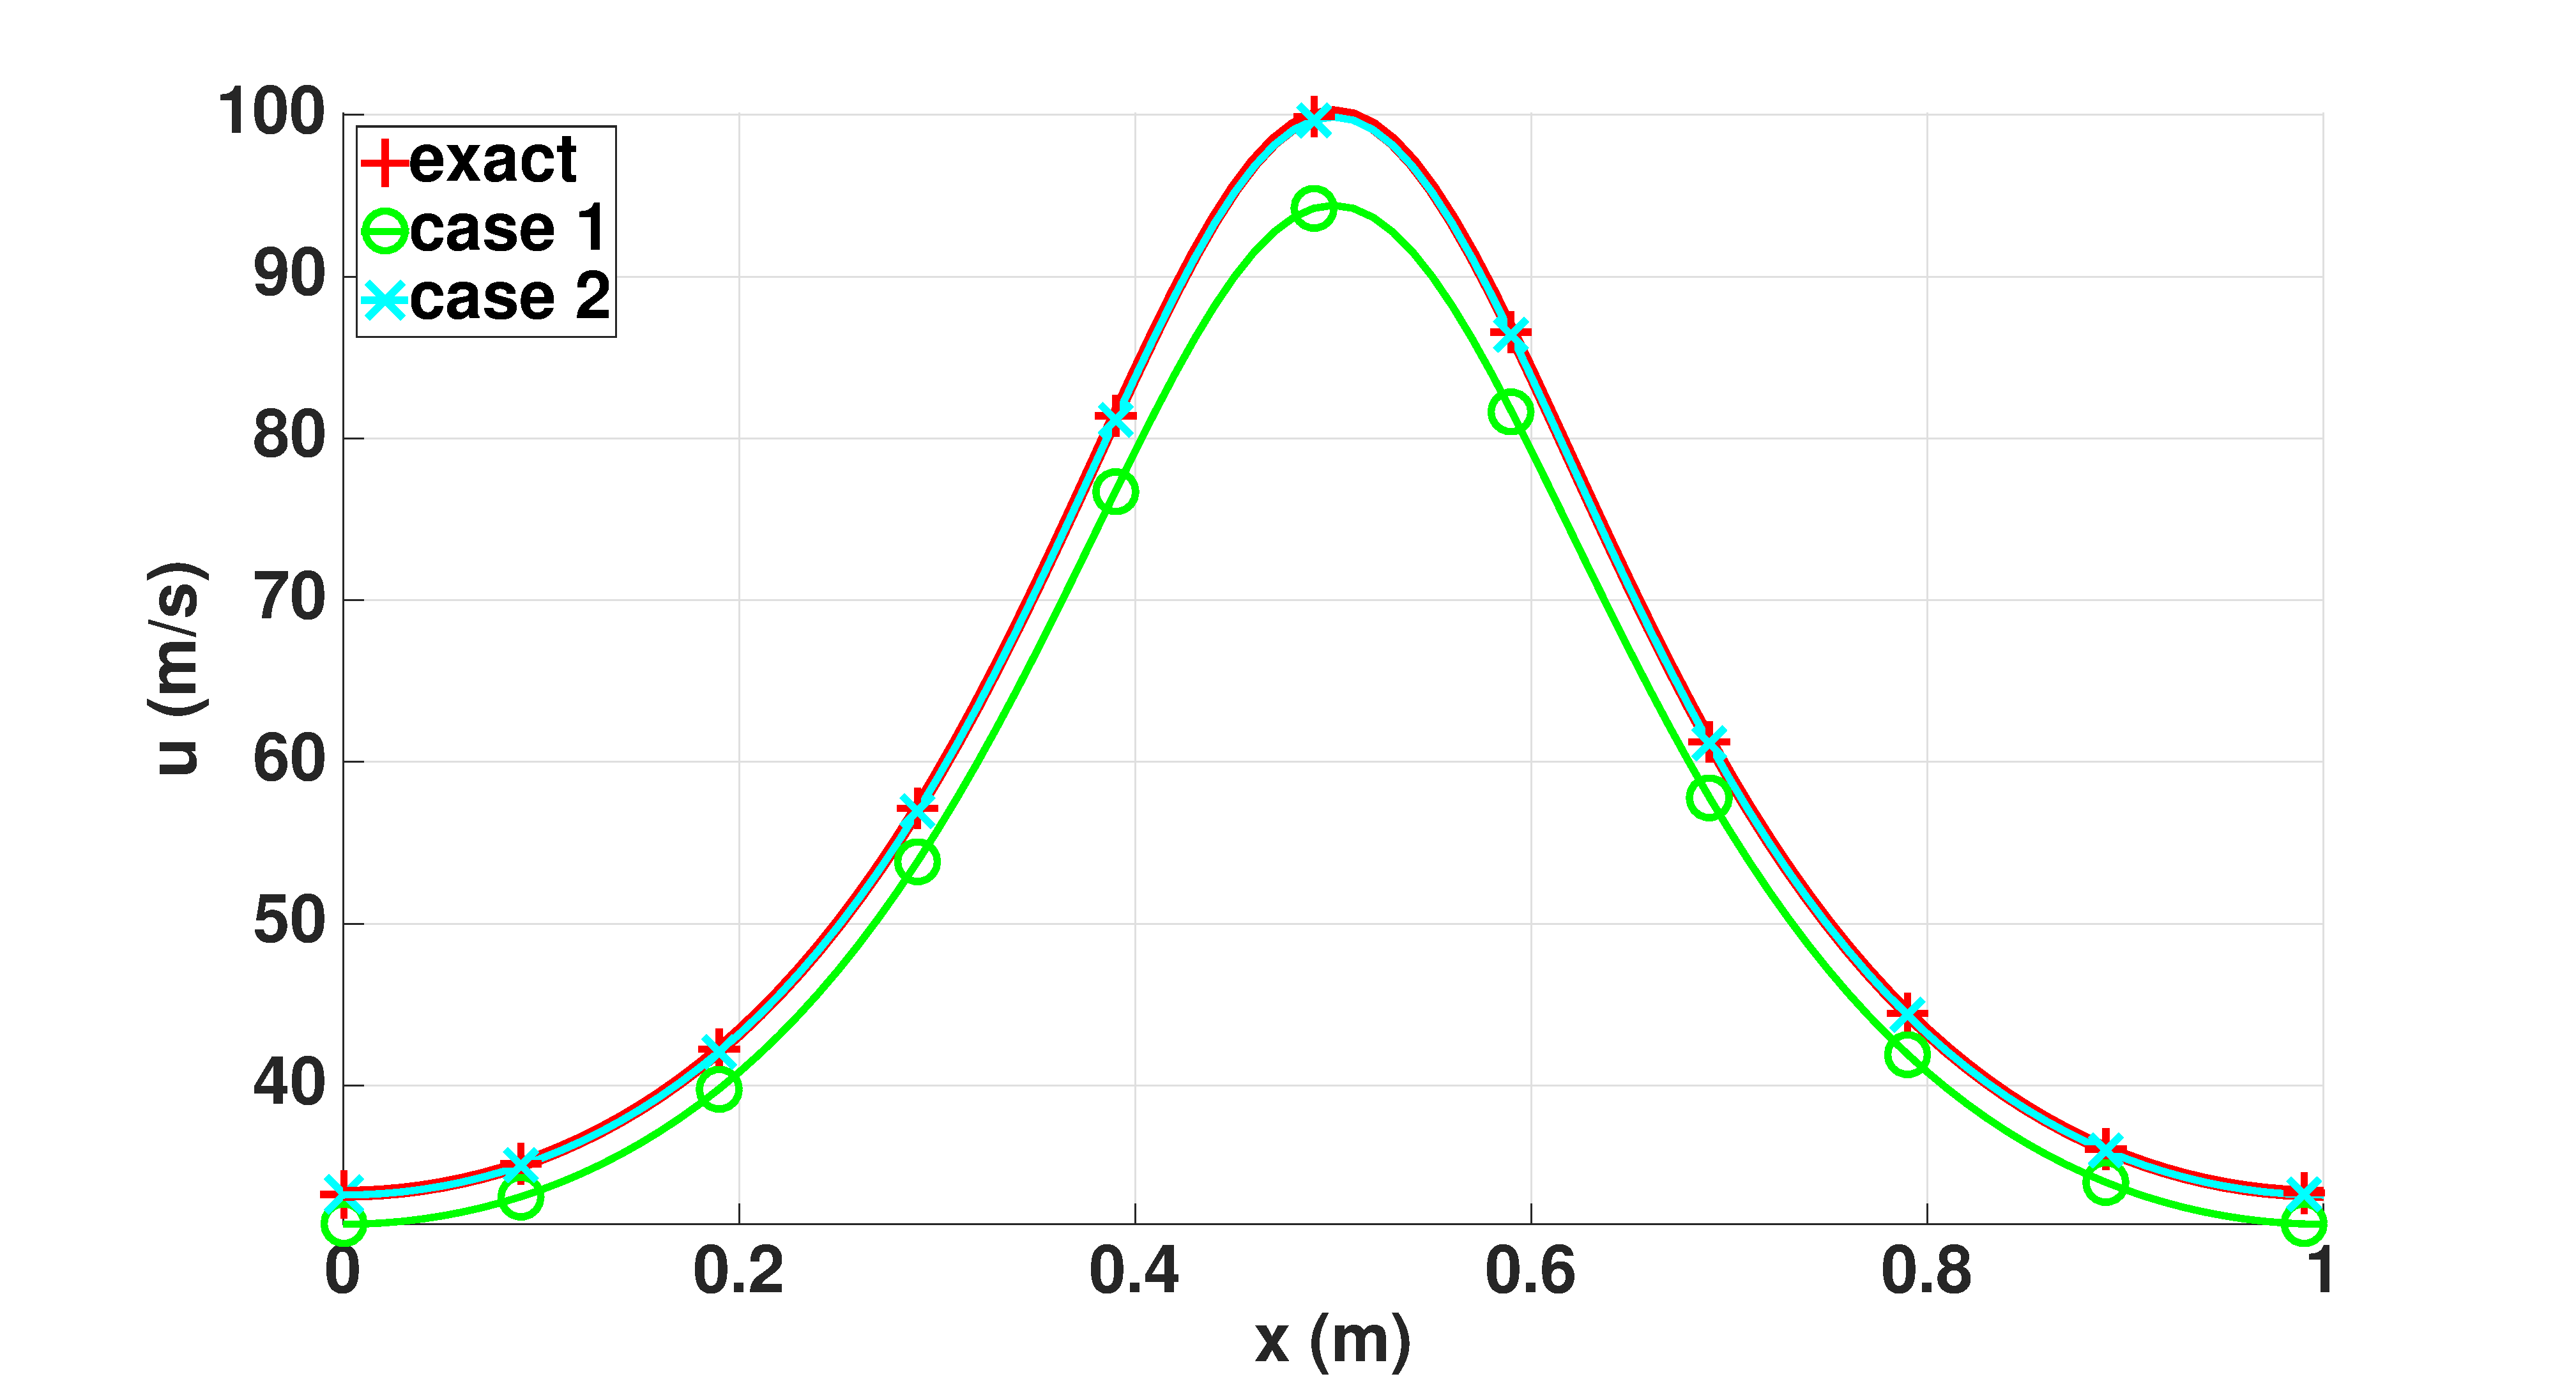
\includegraphics[width=\textwidth]{figures/liquid_velocity_llf_and_exact_100.eps}
                \caption{Velocity}
                \label{fig:liq-phase-vel}
        \end{subfigure}%
        \begin{subfigure}[b]{0.5\textwidth}
                \centering
                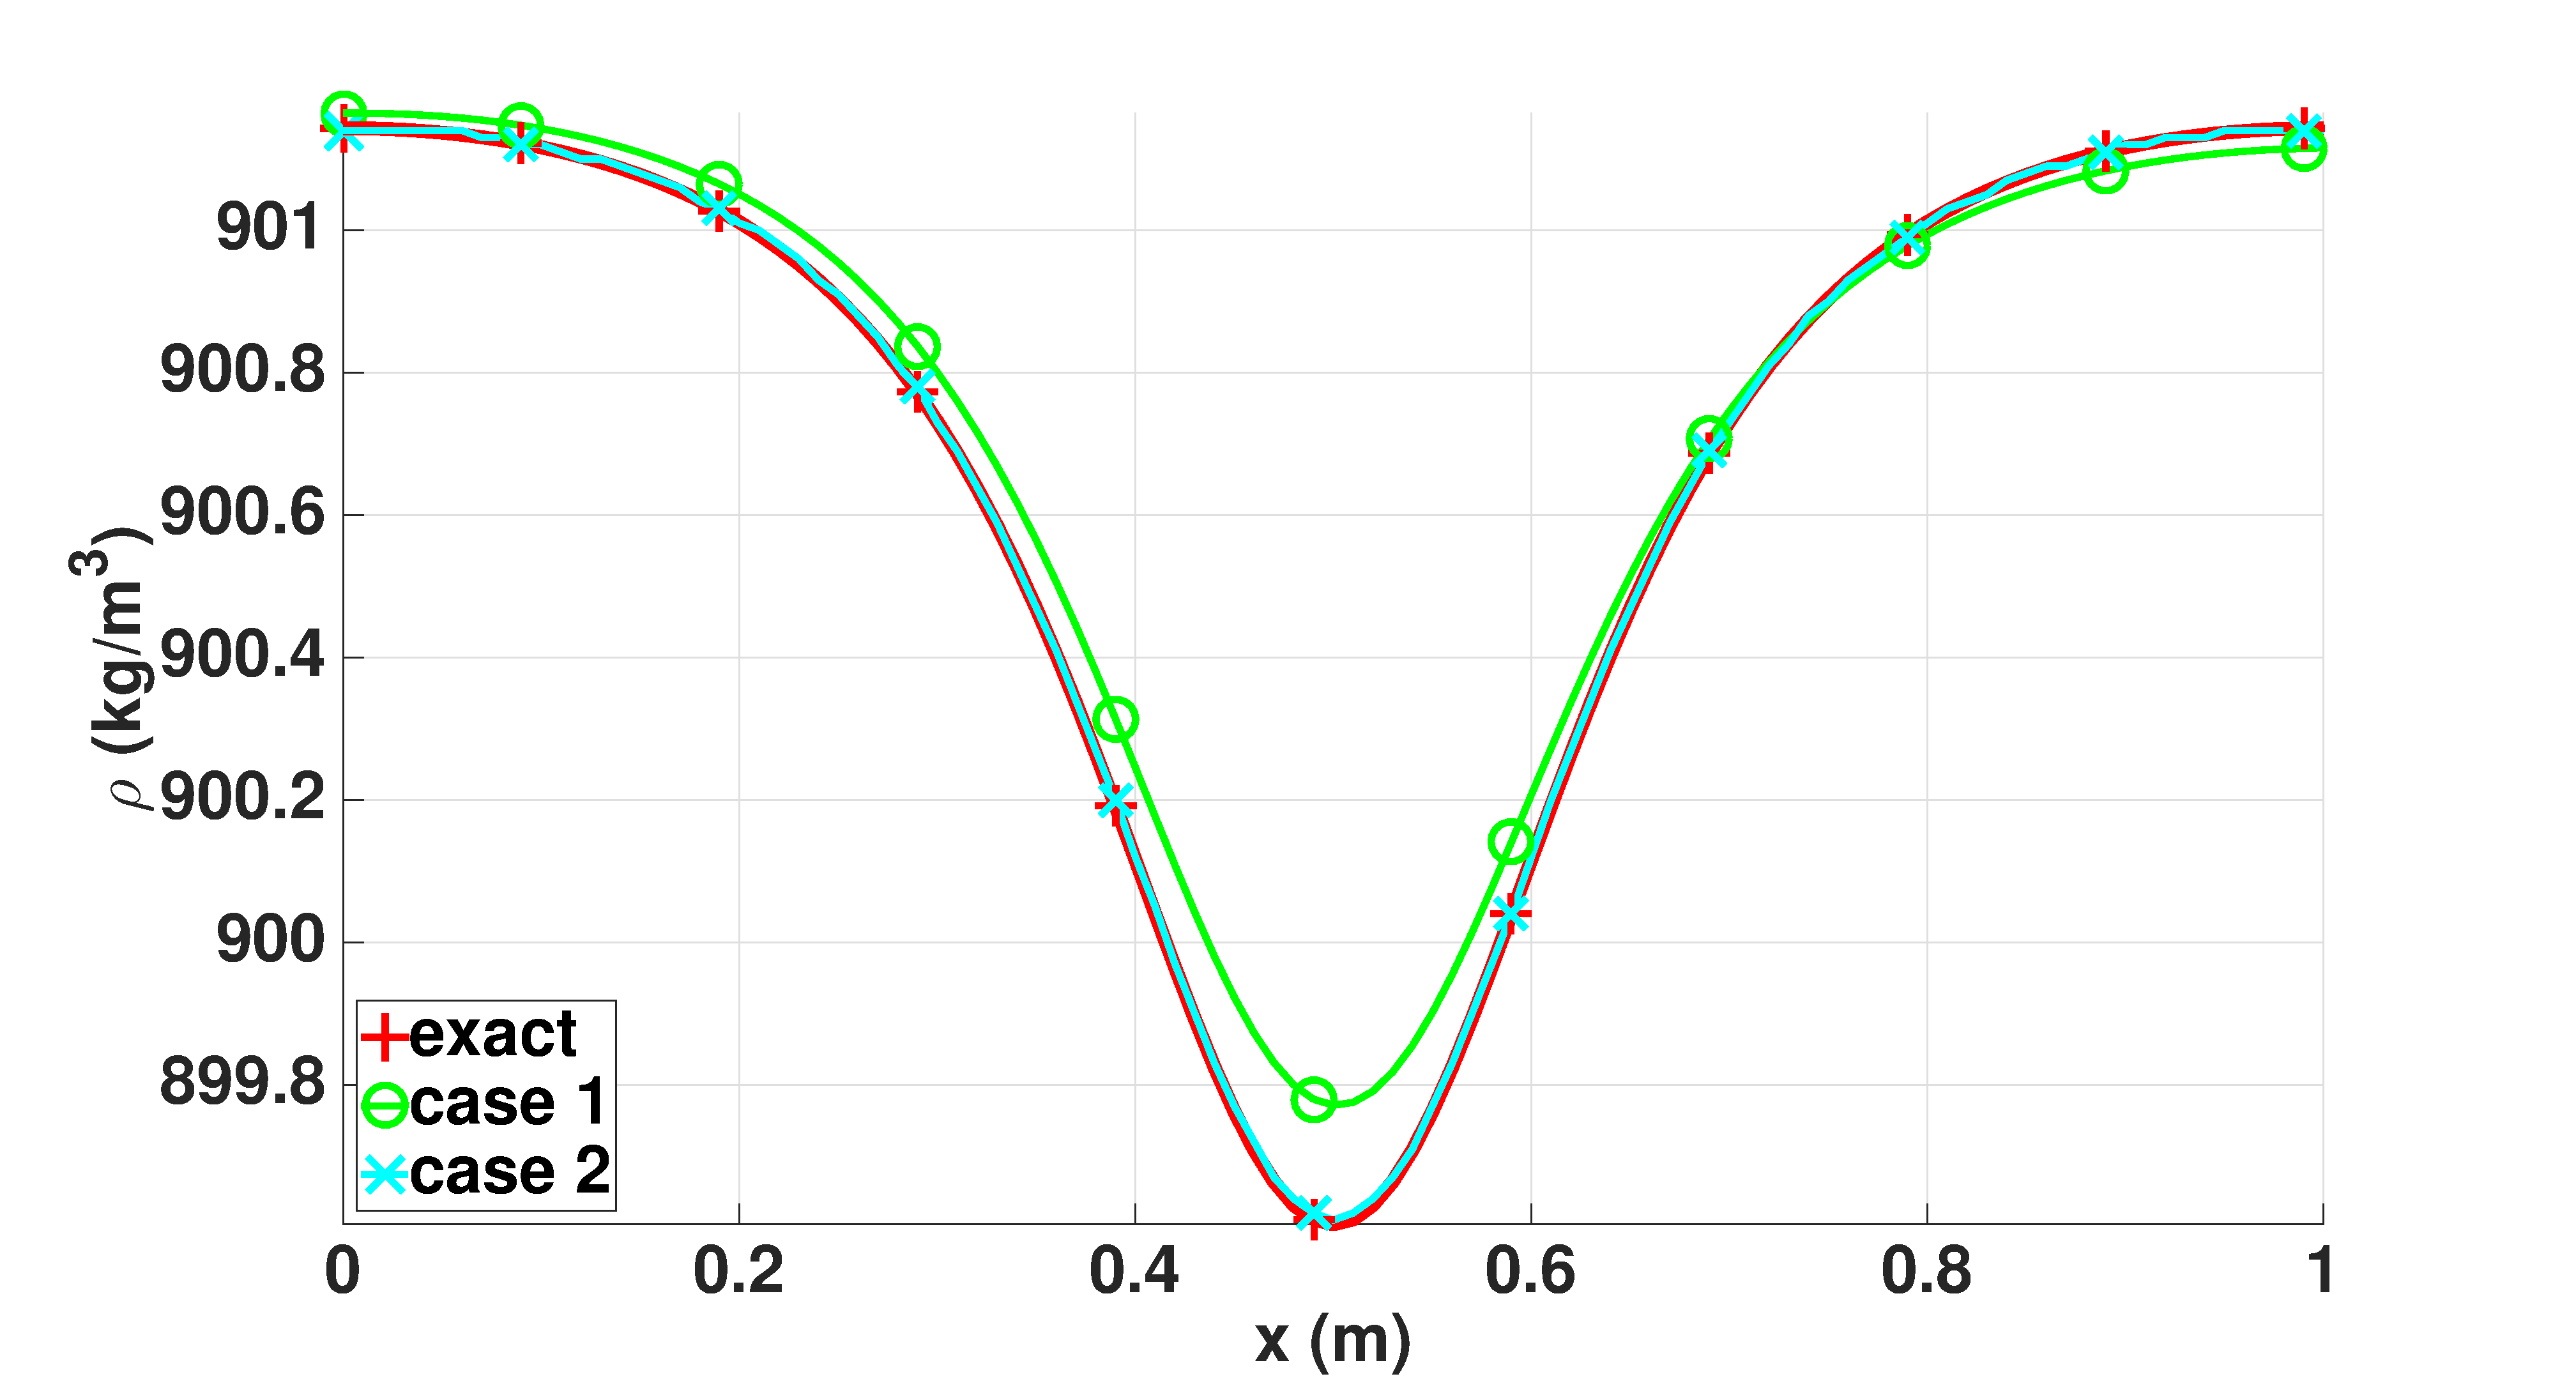
\includegraphics[width=\textwidth]{figures/liquid_density_llf_and_exact_100.eps}
                \caption{Density}
                \label{fig:liq-phase-density}
        \end{subfigure}
        
        \begin{subfigure}[b]{0.495\textwidth}
                \centering
                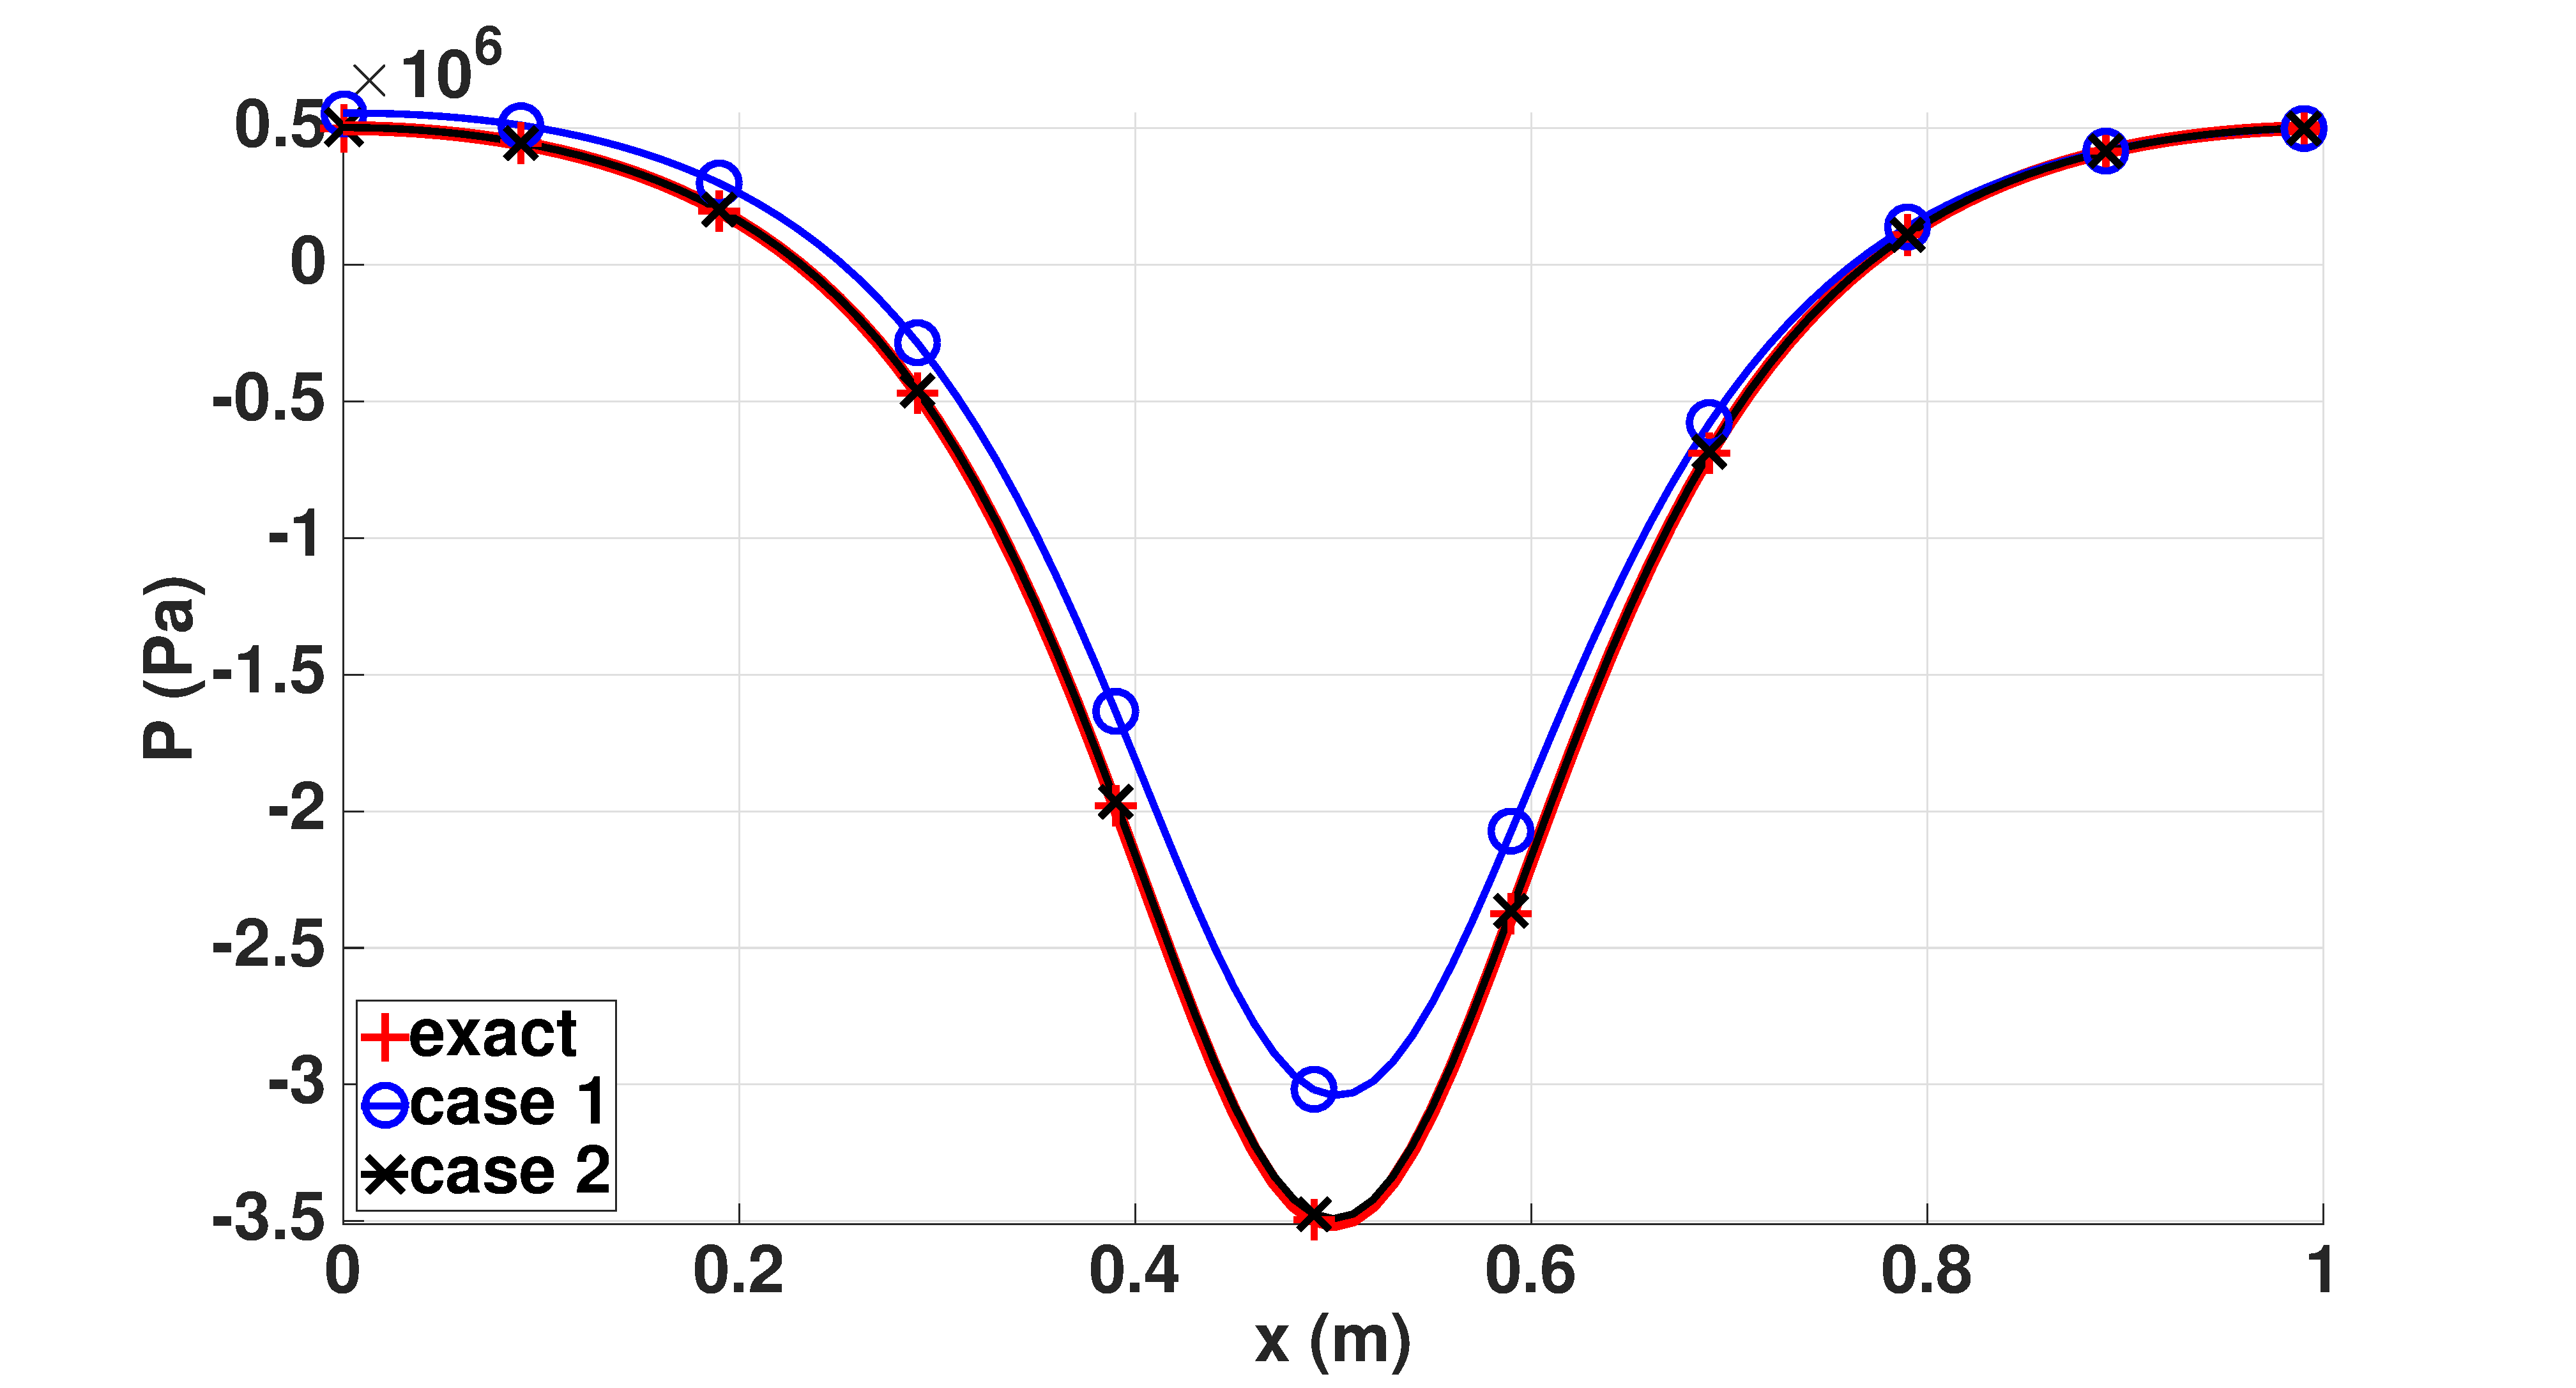
\includegraphics[width=\textwidth]{figures/liquid_pressure_llf_and_exact_100.eps}
                \caption{Pressure}
                \label{fig:liq-phase-press}
        \end{subfigure}        
        \begin{subfigure}[b]{0.495\textwidth}
                \centering
                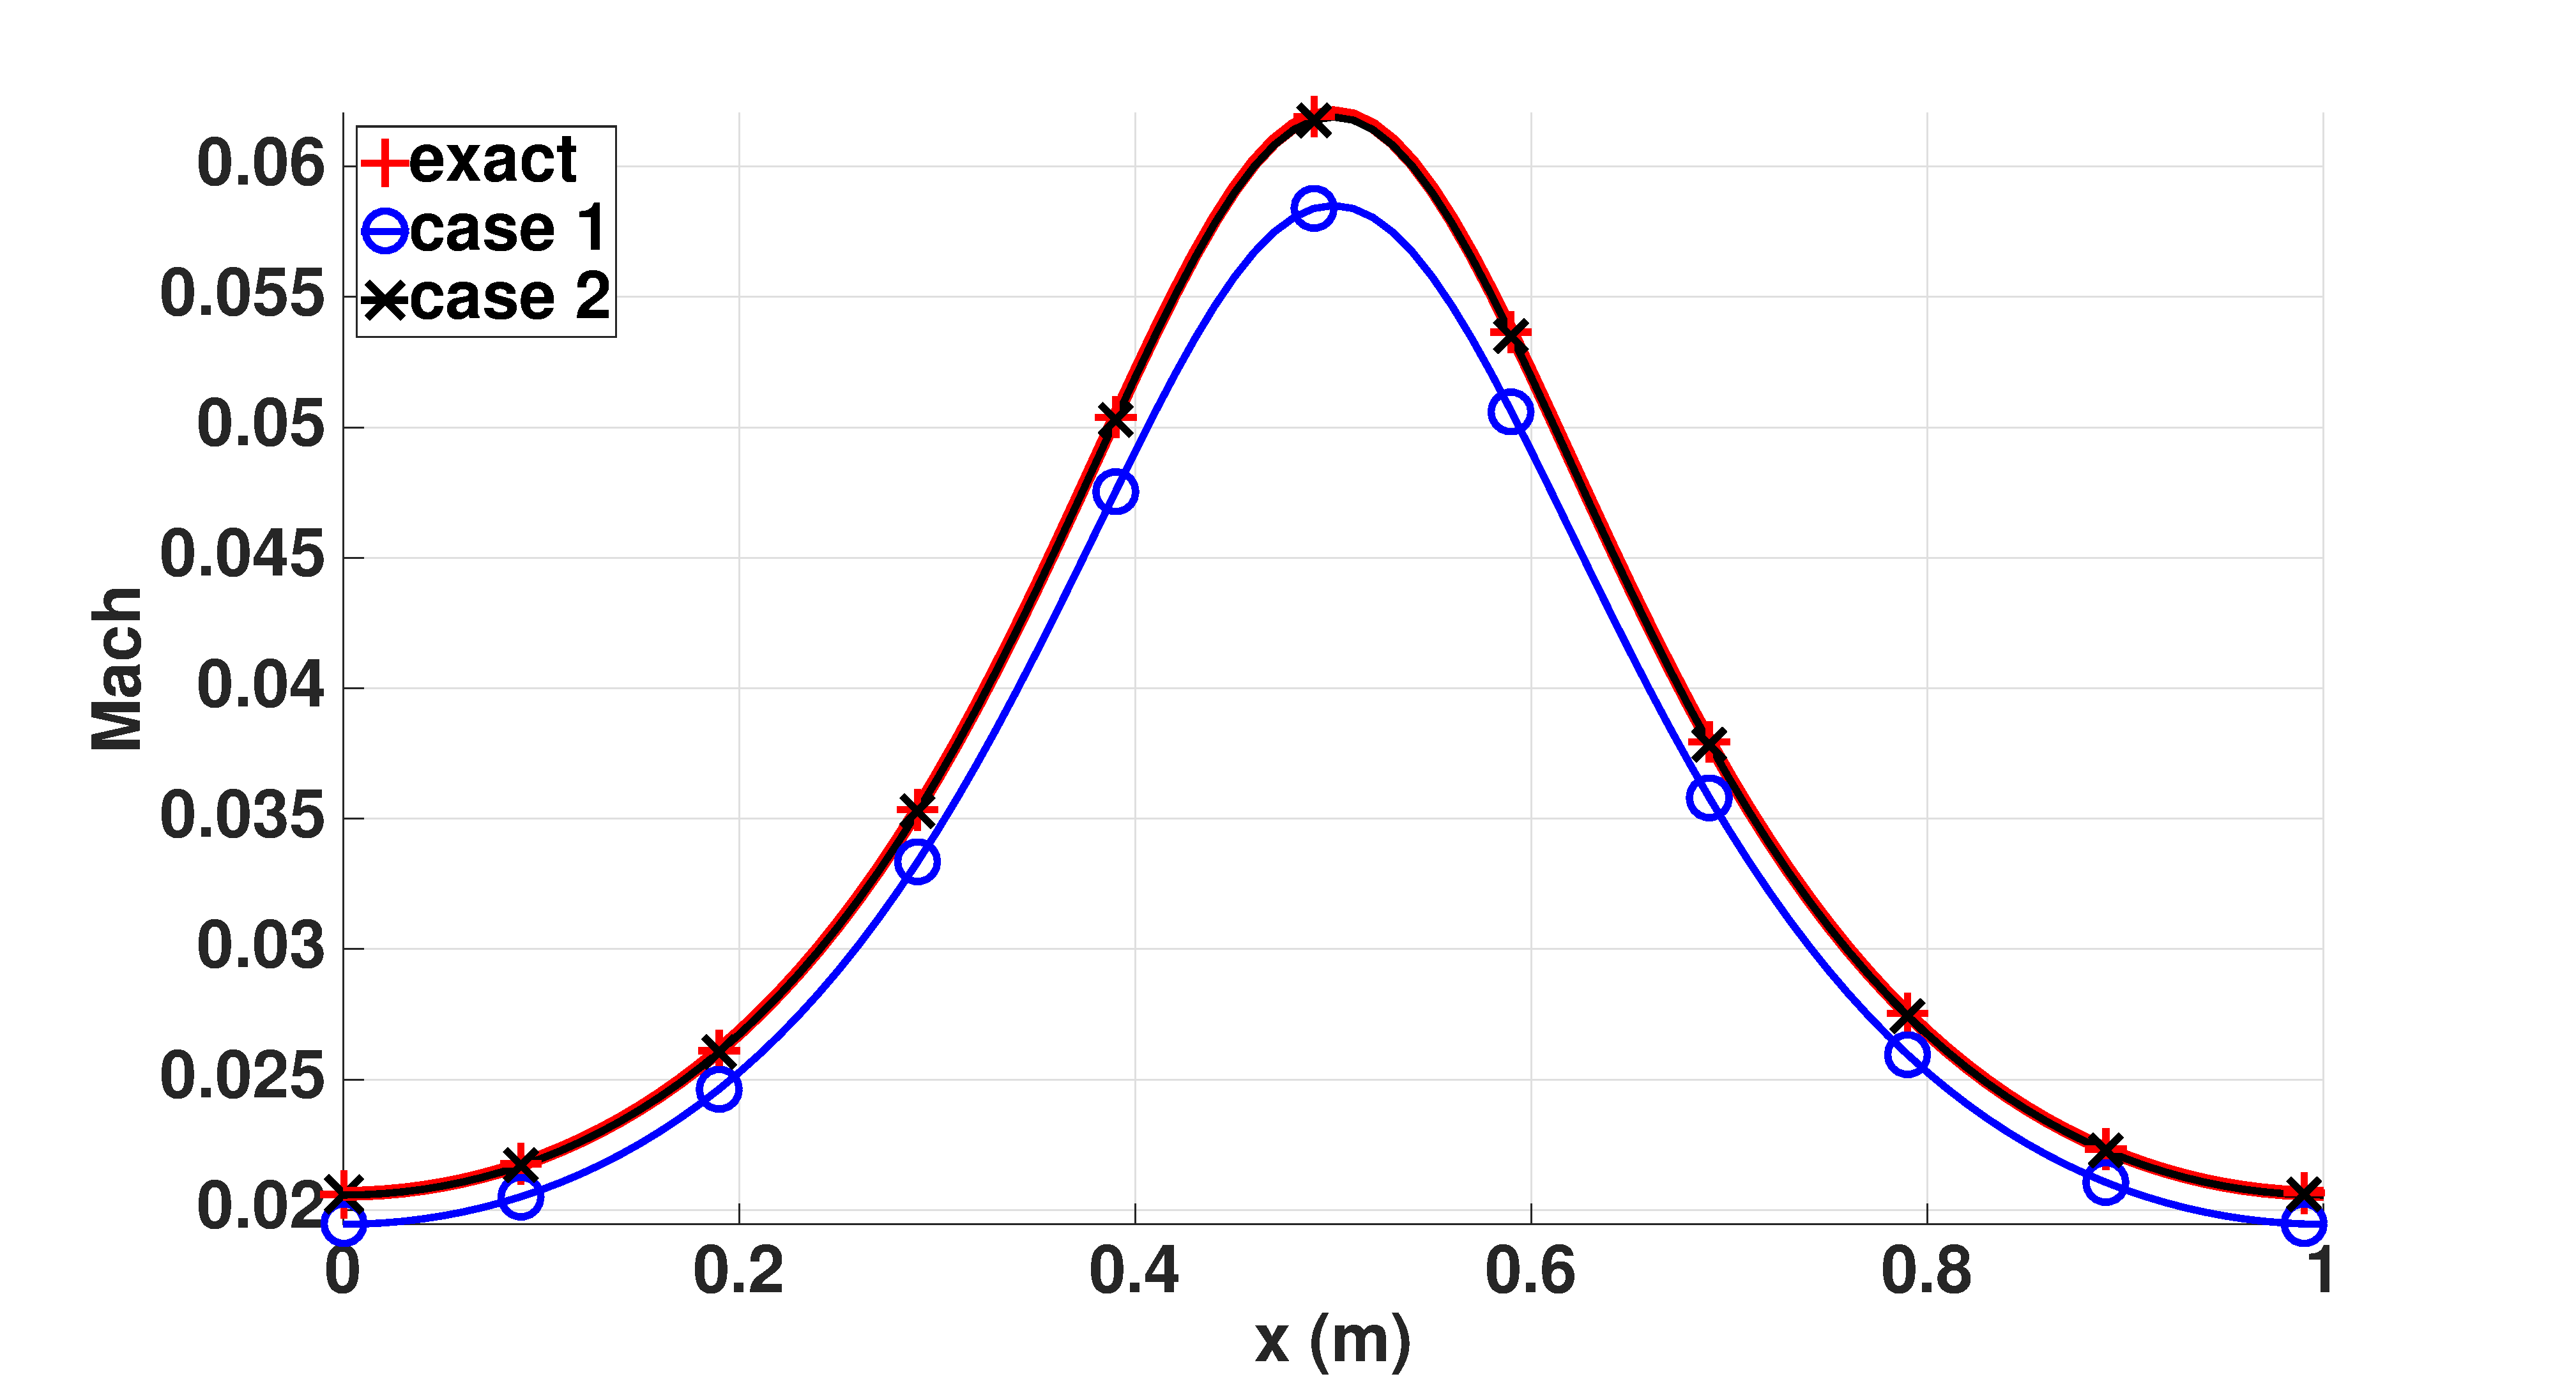
\includegraphics[width=\textwidth]{figures/liquid_mach_llf_and_exact_100.eps}
                \caption{Mach number}
                \label{fig:liq-phase-mach}
        \end{subfigure}
        \caption{Numerical and analytical steady-state liquid-phase solutions for the divergent-convergent two-phase flow nozzle problem.}\label{fig:liq-phase}
\end{figure}
%
The steady-state numerical solution of the liquid phase is shown in \fig{fig:liq-phase}.
In case (1) (LLF viscosity without a low-Mach fix), the numerical solution does not match the exact solution; this illustrates the ill-scaling effect of the 
dissipative terms for low-Mach flows (see Mach plot in  \fig{fig:liq-phase-mach}). The numerical solution obtained in case (2) (LLF viscosity with low-Mach fix,
i.e., properly scaled LLF viscosity) converges to the exact solution and the correct low-Mach asymptotic limit is recovered. 
%Note that in this case, the numerical solution would not be really improved as the mesh in refined since the solution is smooth. 
%

%----------------------------------------------------------
\subsection{Shock tube with nearly pure phases}\label{sec:third-test}
%-----------------------------------------------------------
%
%
Finally, we conclude with a liquid-gas shock tube where the two phase are initially in their nearly pure state 
($\alpha_l = \varepsilon = 5\times 10^{-4}$ for $x<0.5$ and $\alpha_l = 1- \varepsilon $ for $x>0.5$). 
The initial conditions are: $P_{\text{left}}=2\times 10^8$ Pa, $P_{\text{right}}=10^5$ Pa; 
the densities are uniform, $\rho_l = 1000$ kg/m$^3$,  $\rho_v = 50$ kg/m$^3$.  We use the stiffened gas equation of state with the 
following parameters: $\gamma_g=1.4$, $\gamma_l=4.4$, $P_{l,\infty}=6\times 10^8$ Pa, $P_{g,\infty}=0$ Pa , $q_g=q_l=0$ J/kg. The pressure
and velocity relaxation coefficients, $\mu_P$ and $\lambda_u$ are large (we use $A_{int}^{max}=10^6$ in \eqt{eq:Aint-sect4}).
We employ 1,000 mesh cells. The results are in \fig{fig:nearly_pure} at time $200\times 10 ^{-6}$ secs. 


\begin{figure}[H]
        \centering
        \begin{subfigure}[b]{0.5\textwidth}
                \centering
                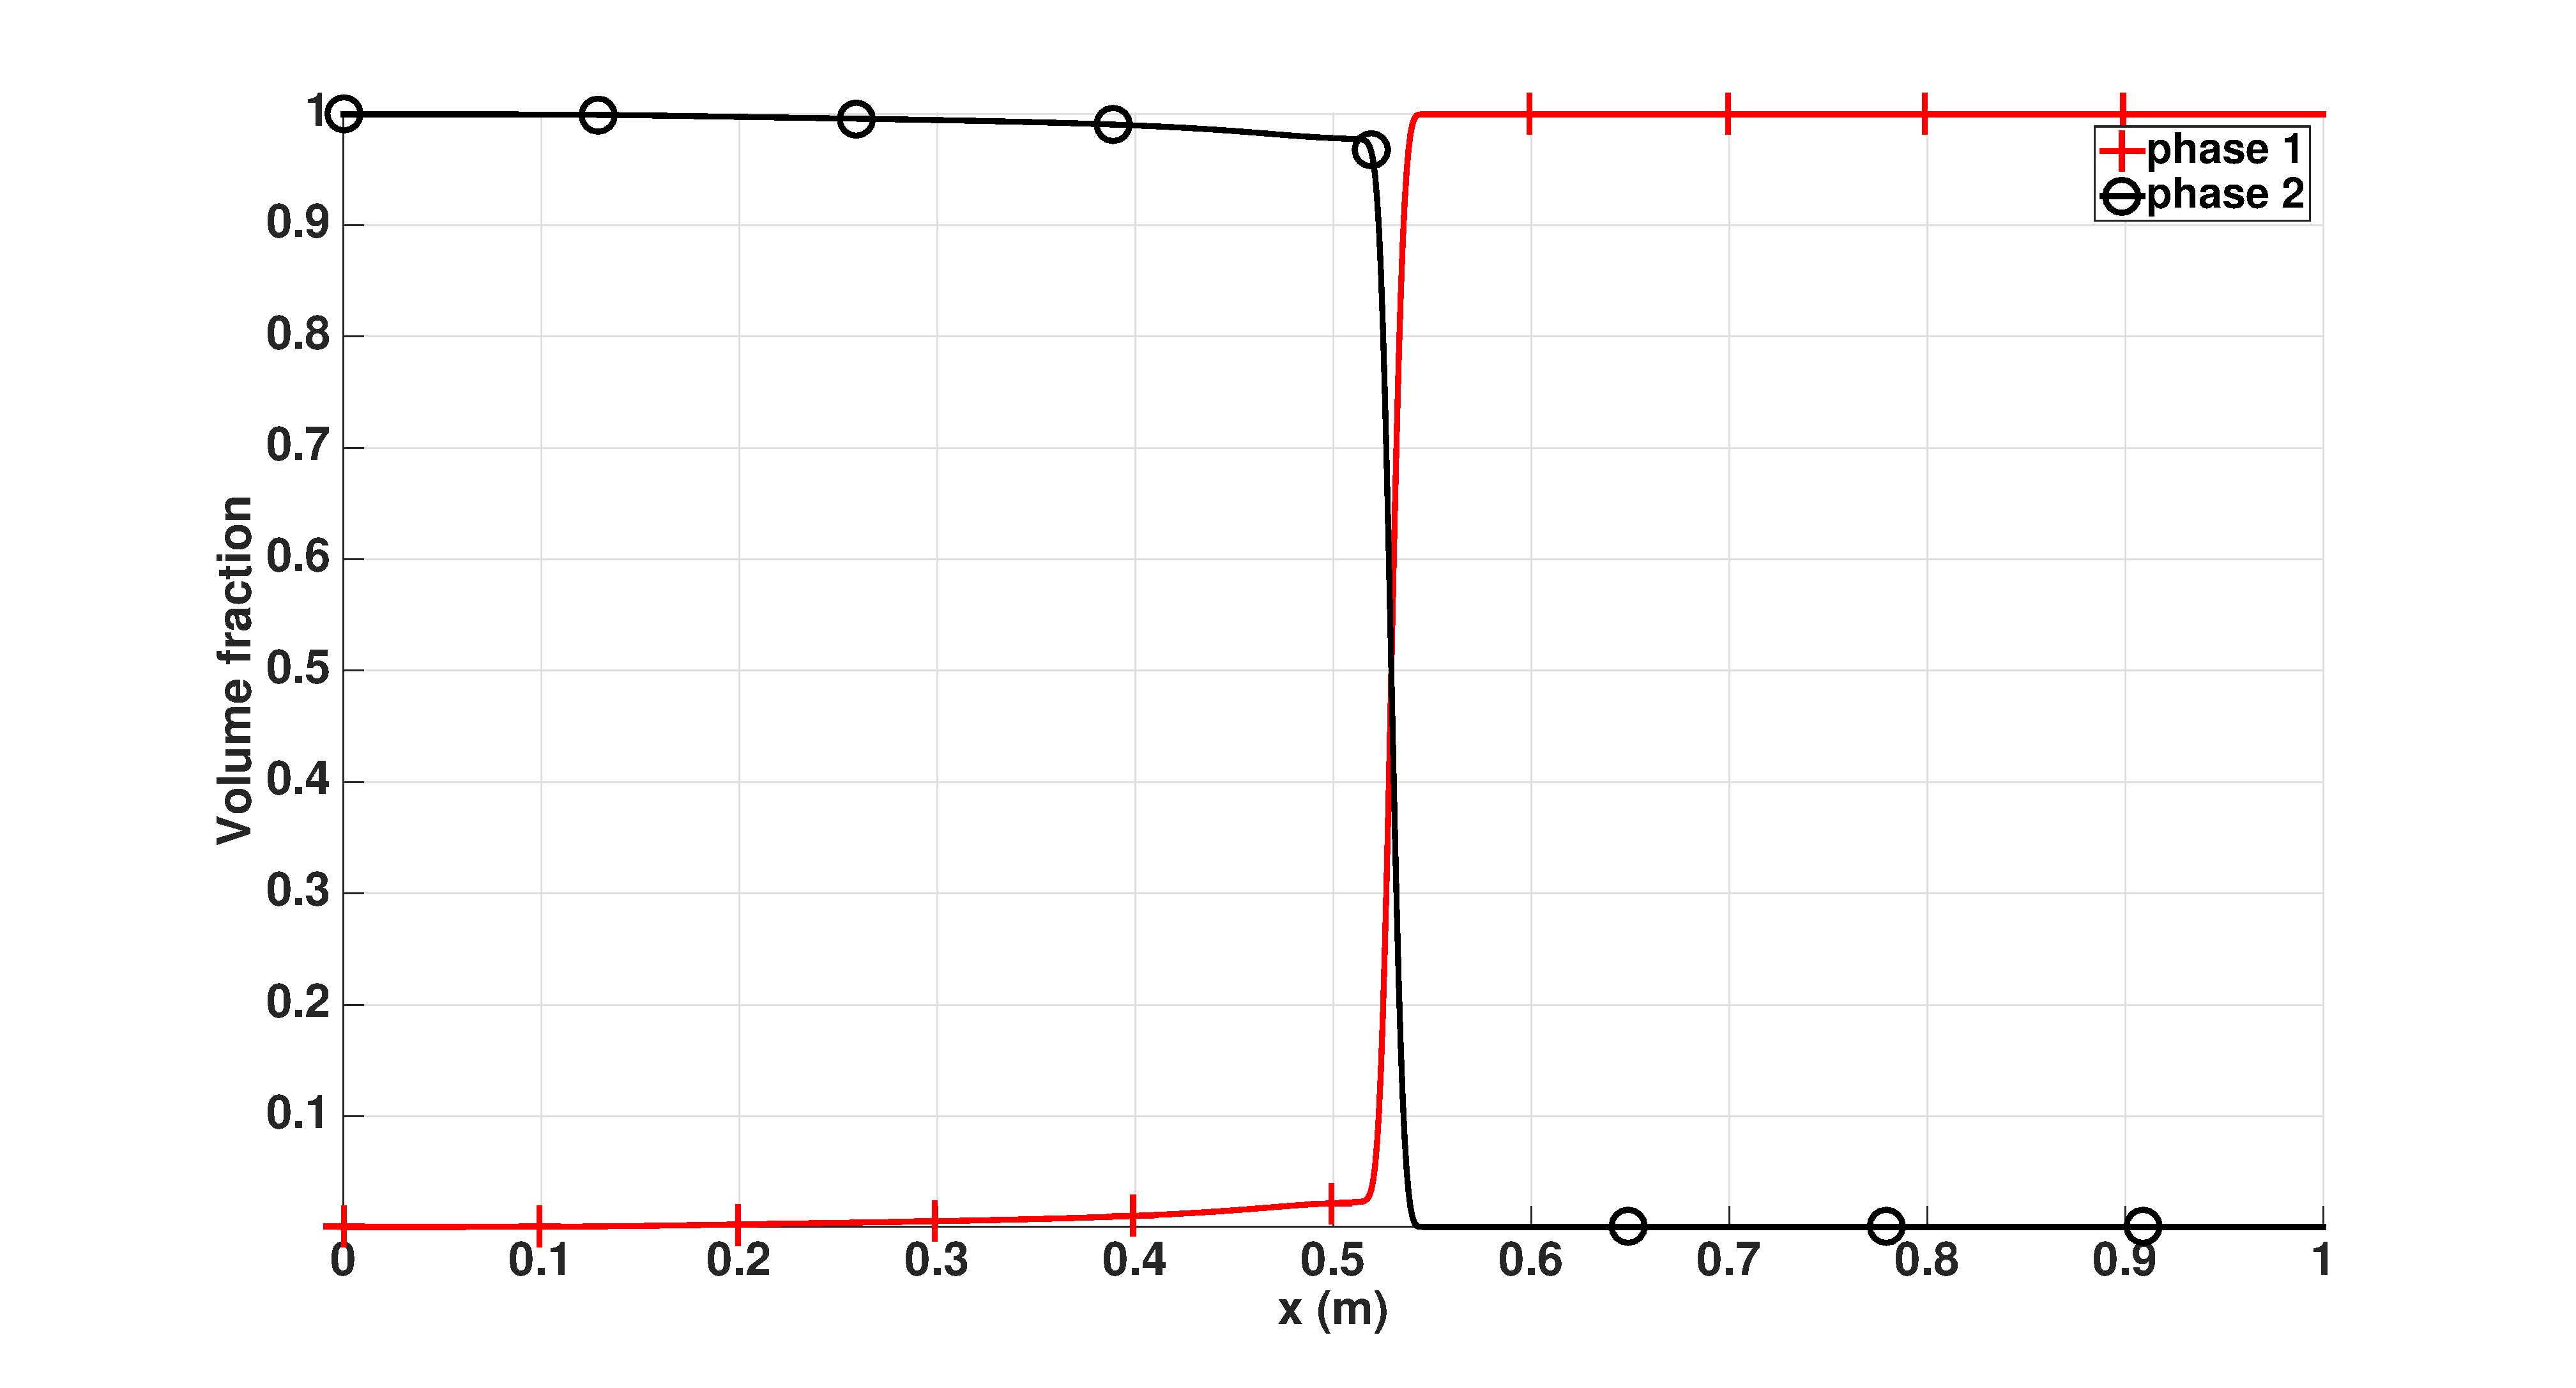
\includegraphics[width=\textwidth]{figures/pure_fluids_infinite_relaxation_two_phases_volume_fraction.eps}
                \caption{Volume fractions}
                \label{fig:nearly_pure_alpha}
        \end{subfigure}%
        \begin{subfigure}[b]{0.5\textwidth}
                \centering
                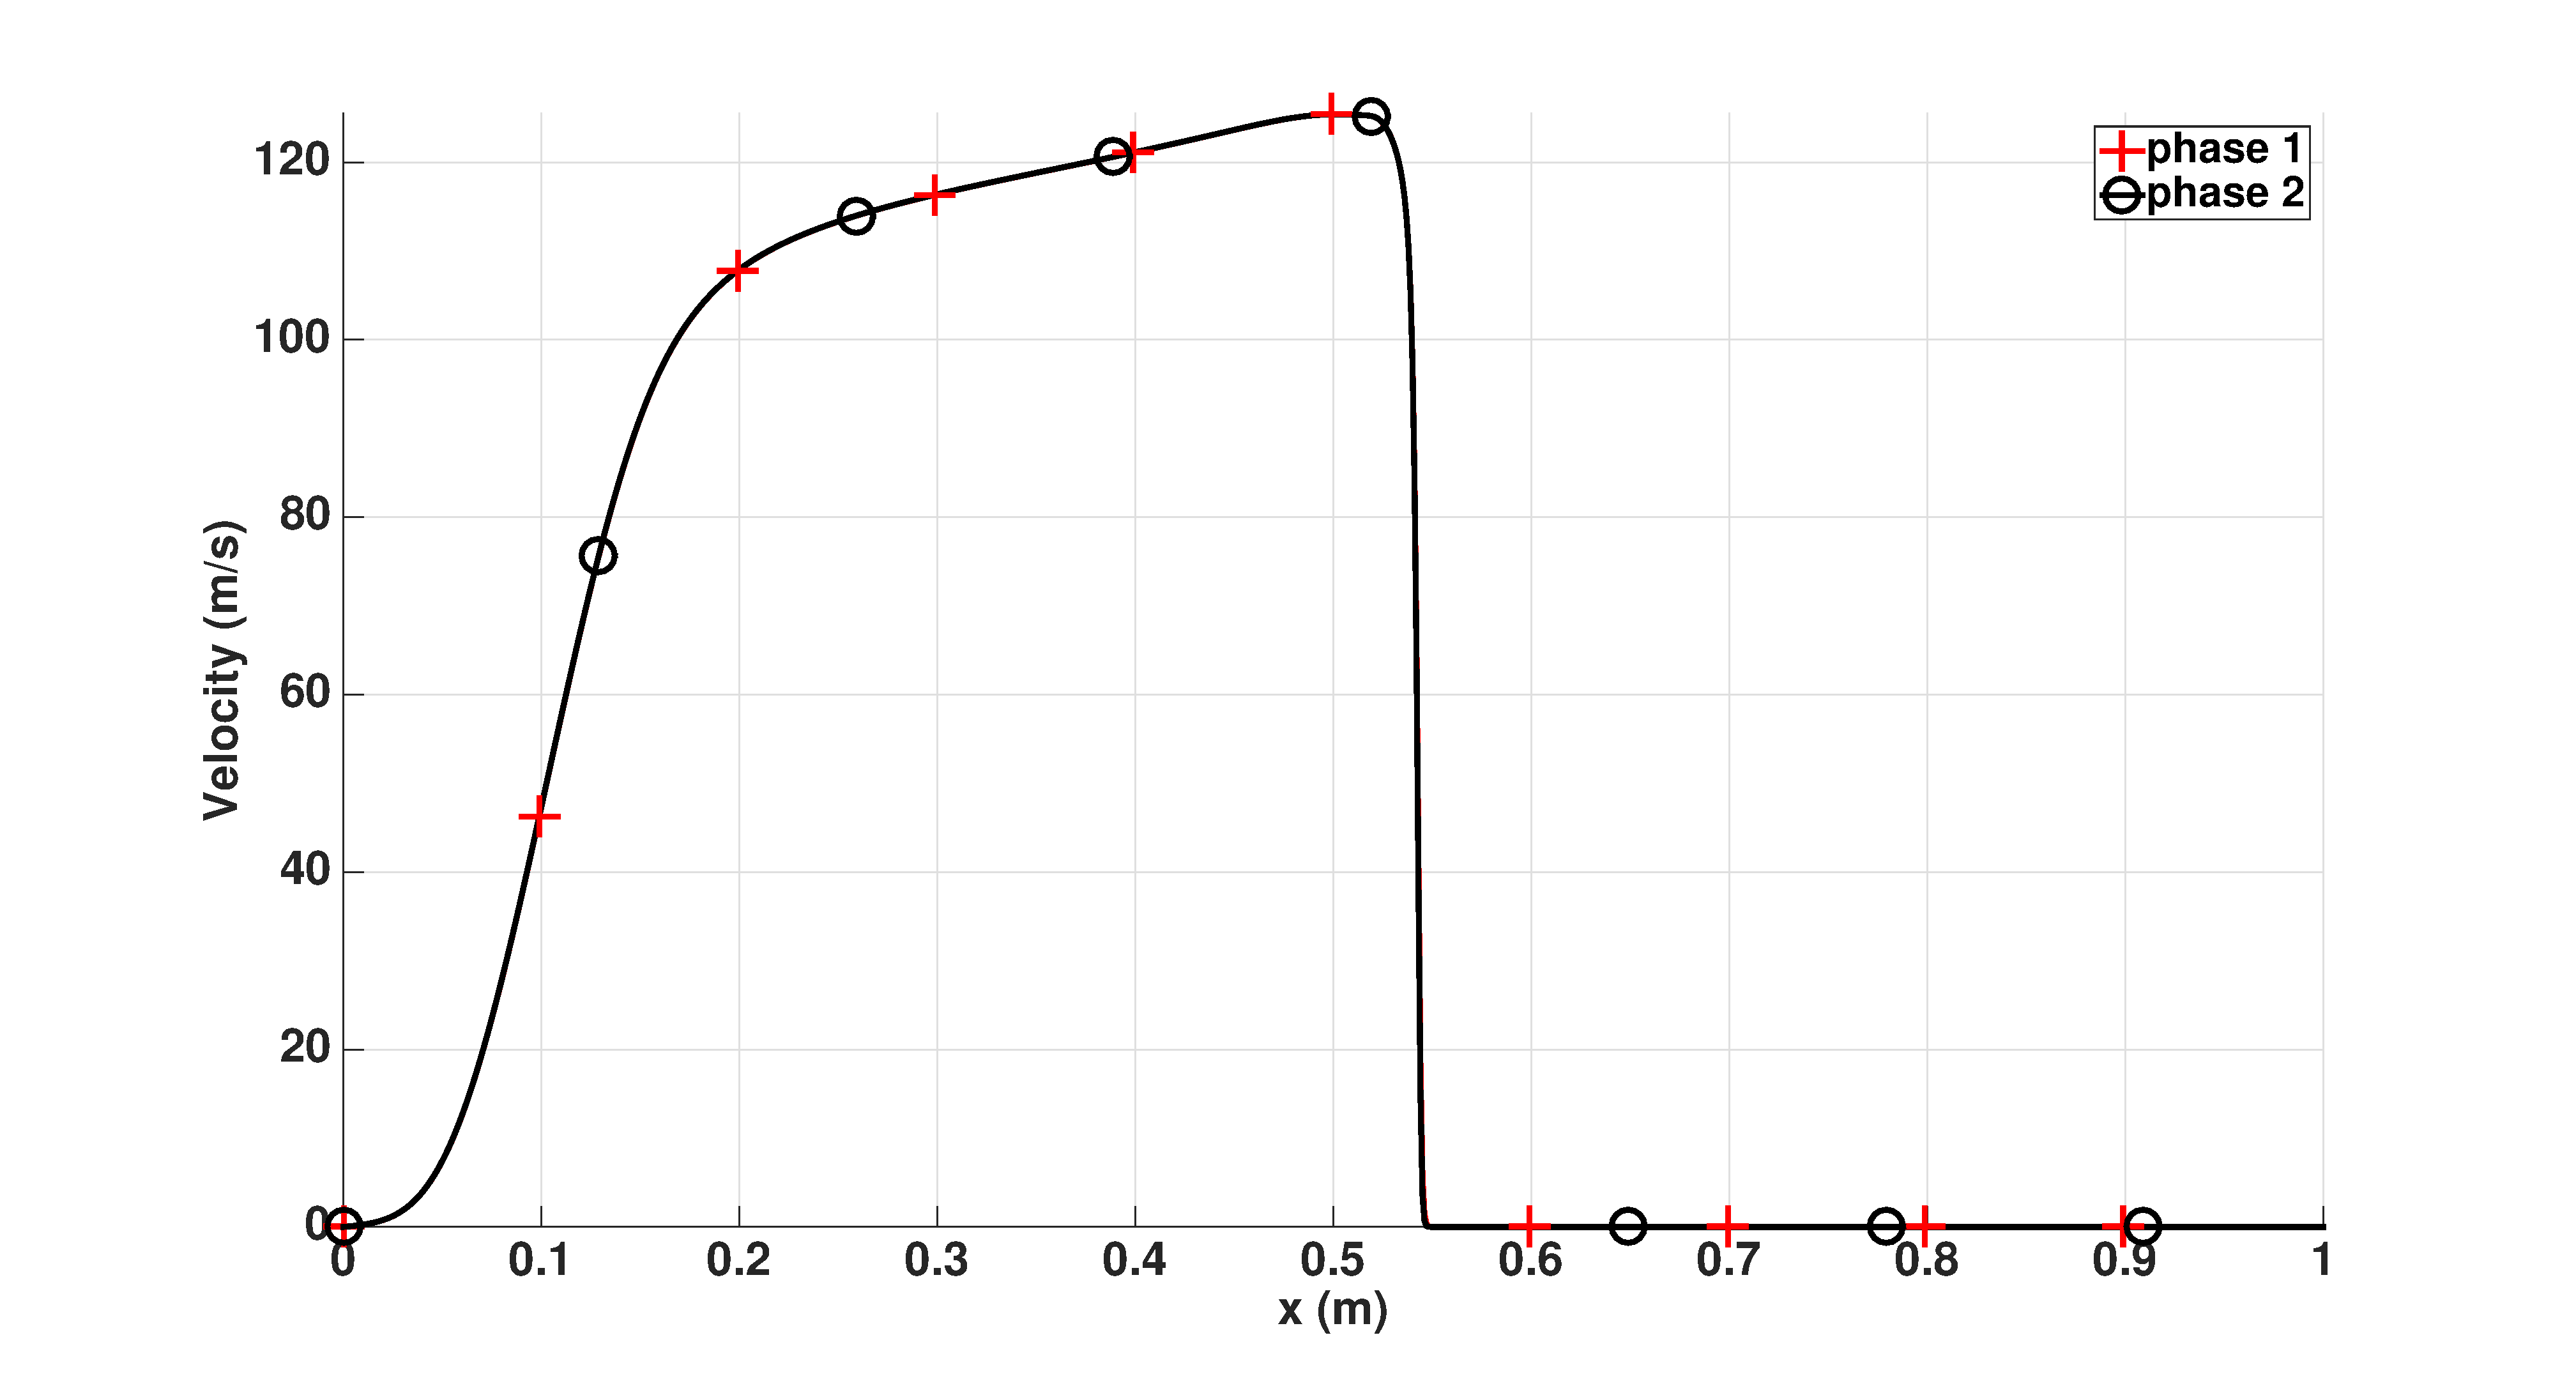
\includegraphics[width=\textwidth]{figures/pure_fluids_infinite_relaxation_two_phases_velocity.eps}
                \caption{Velocities}
                \label{fig:nearly_pure_velocity}
        \end{subfigure}
        
        \begin{subfigure}[b]{0.495\textwidth}
                \centering
                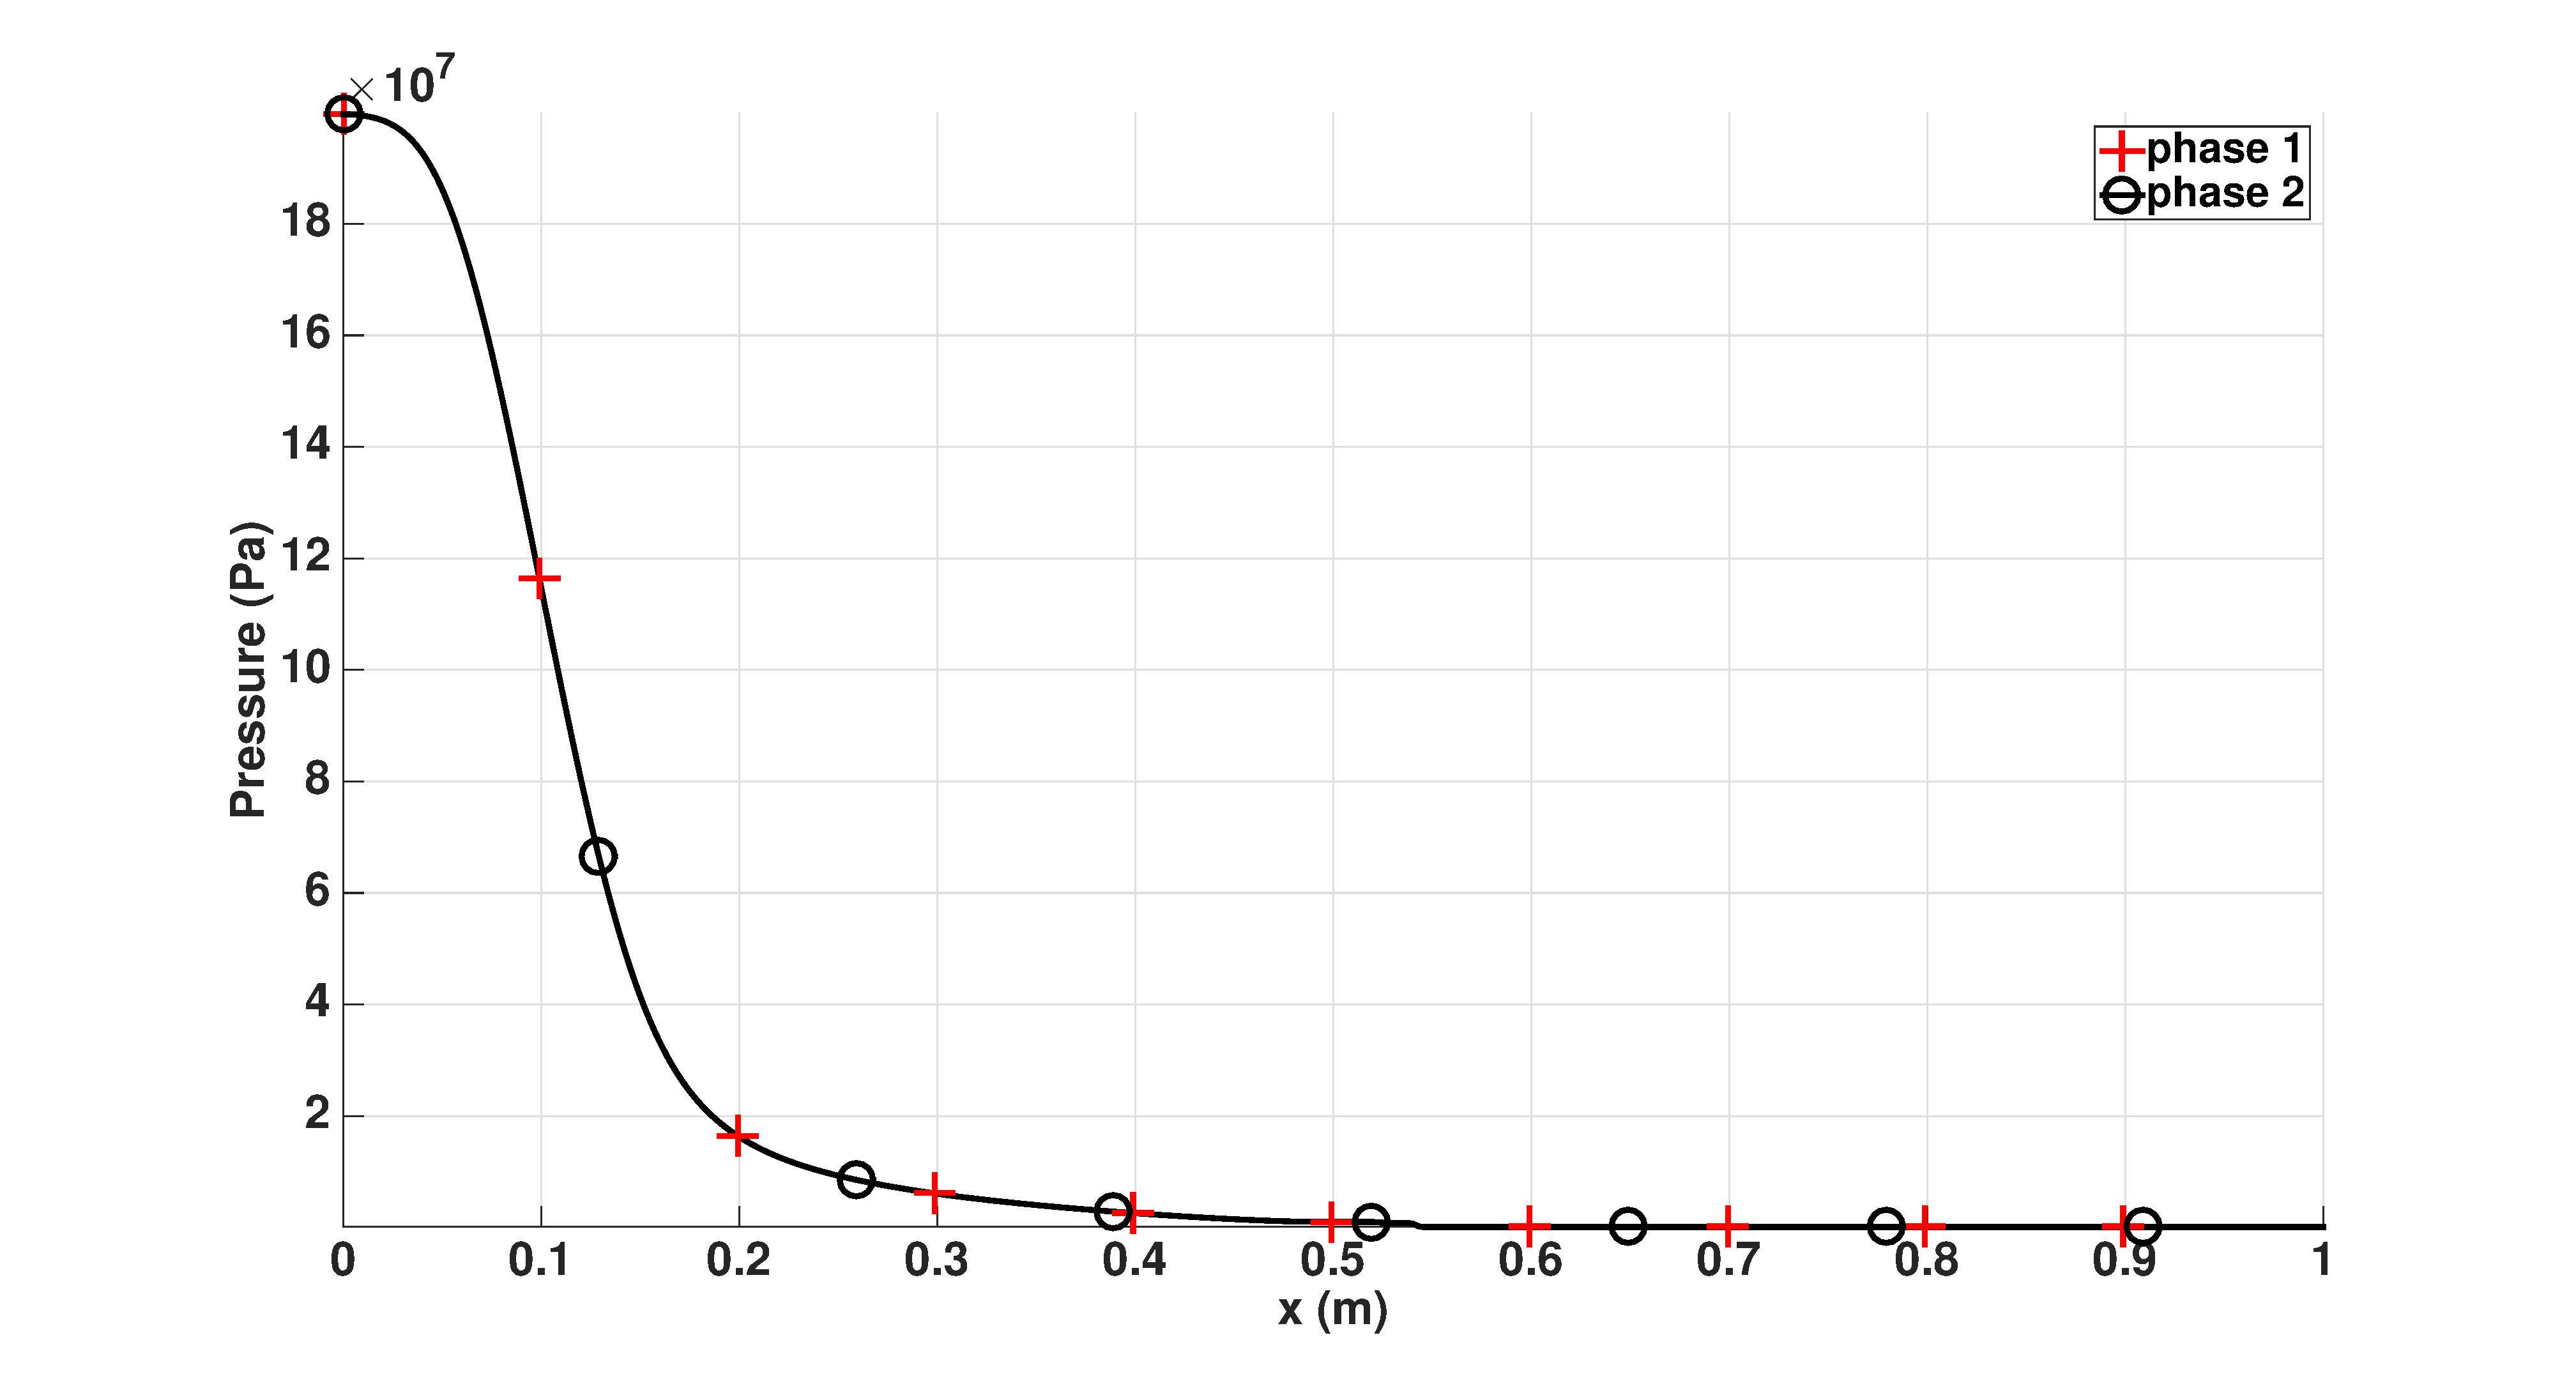
\includegraphics[width=\textwidth]{figures/pure_fluids_infinite_relaxation_two_phases_pressure.eps}
                \caption{Pressures}
                \label{fig:nearly_pure_press}
        \end{subfigure}        
        \begin{subfigure}[b]{0.495\textwidth}
                \centering
                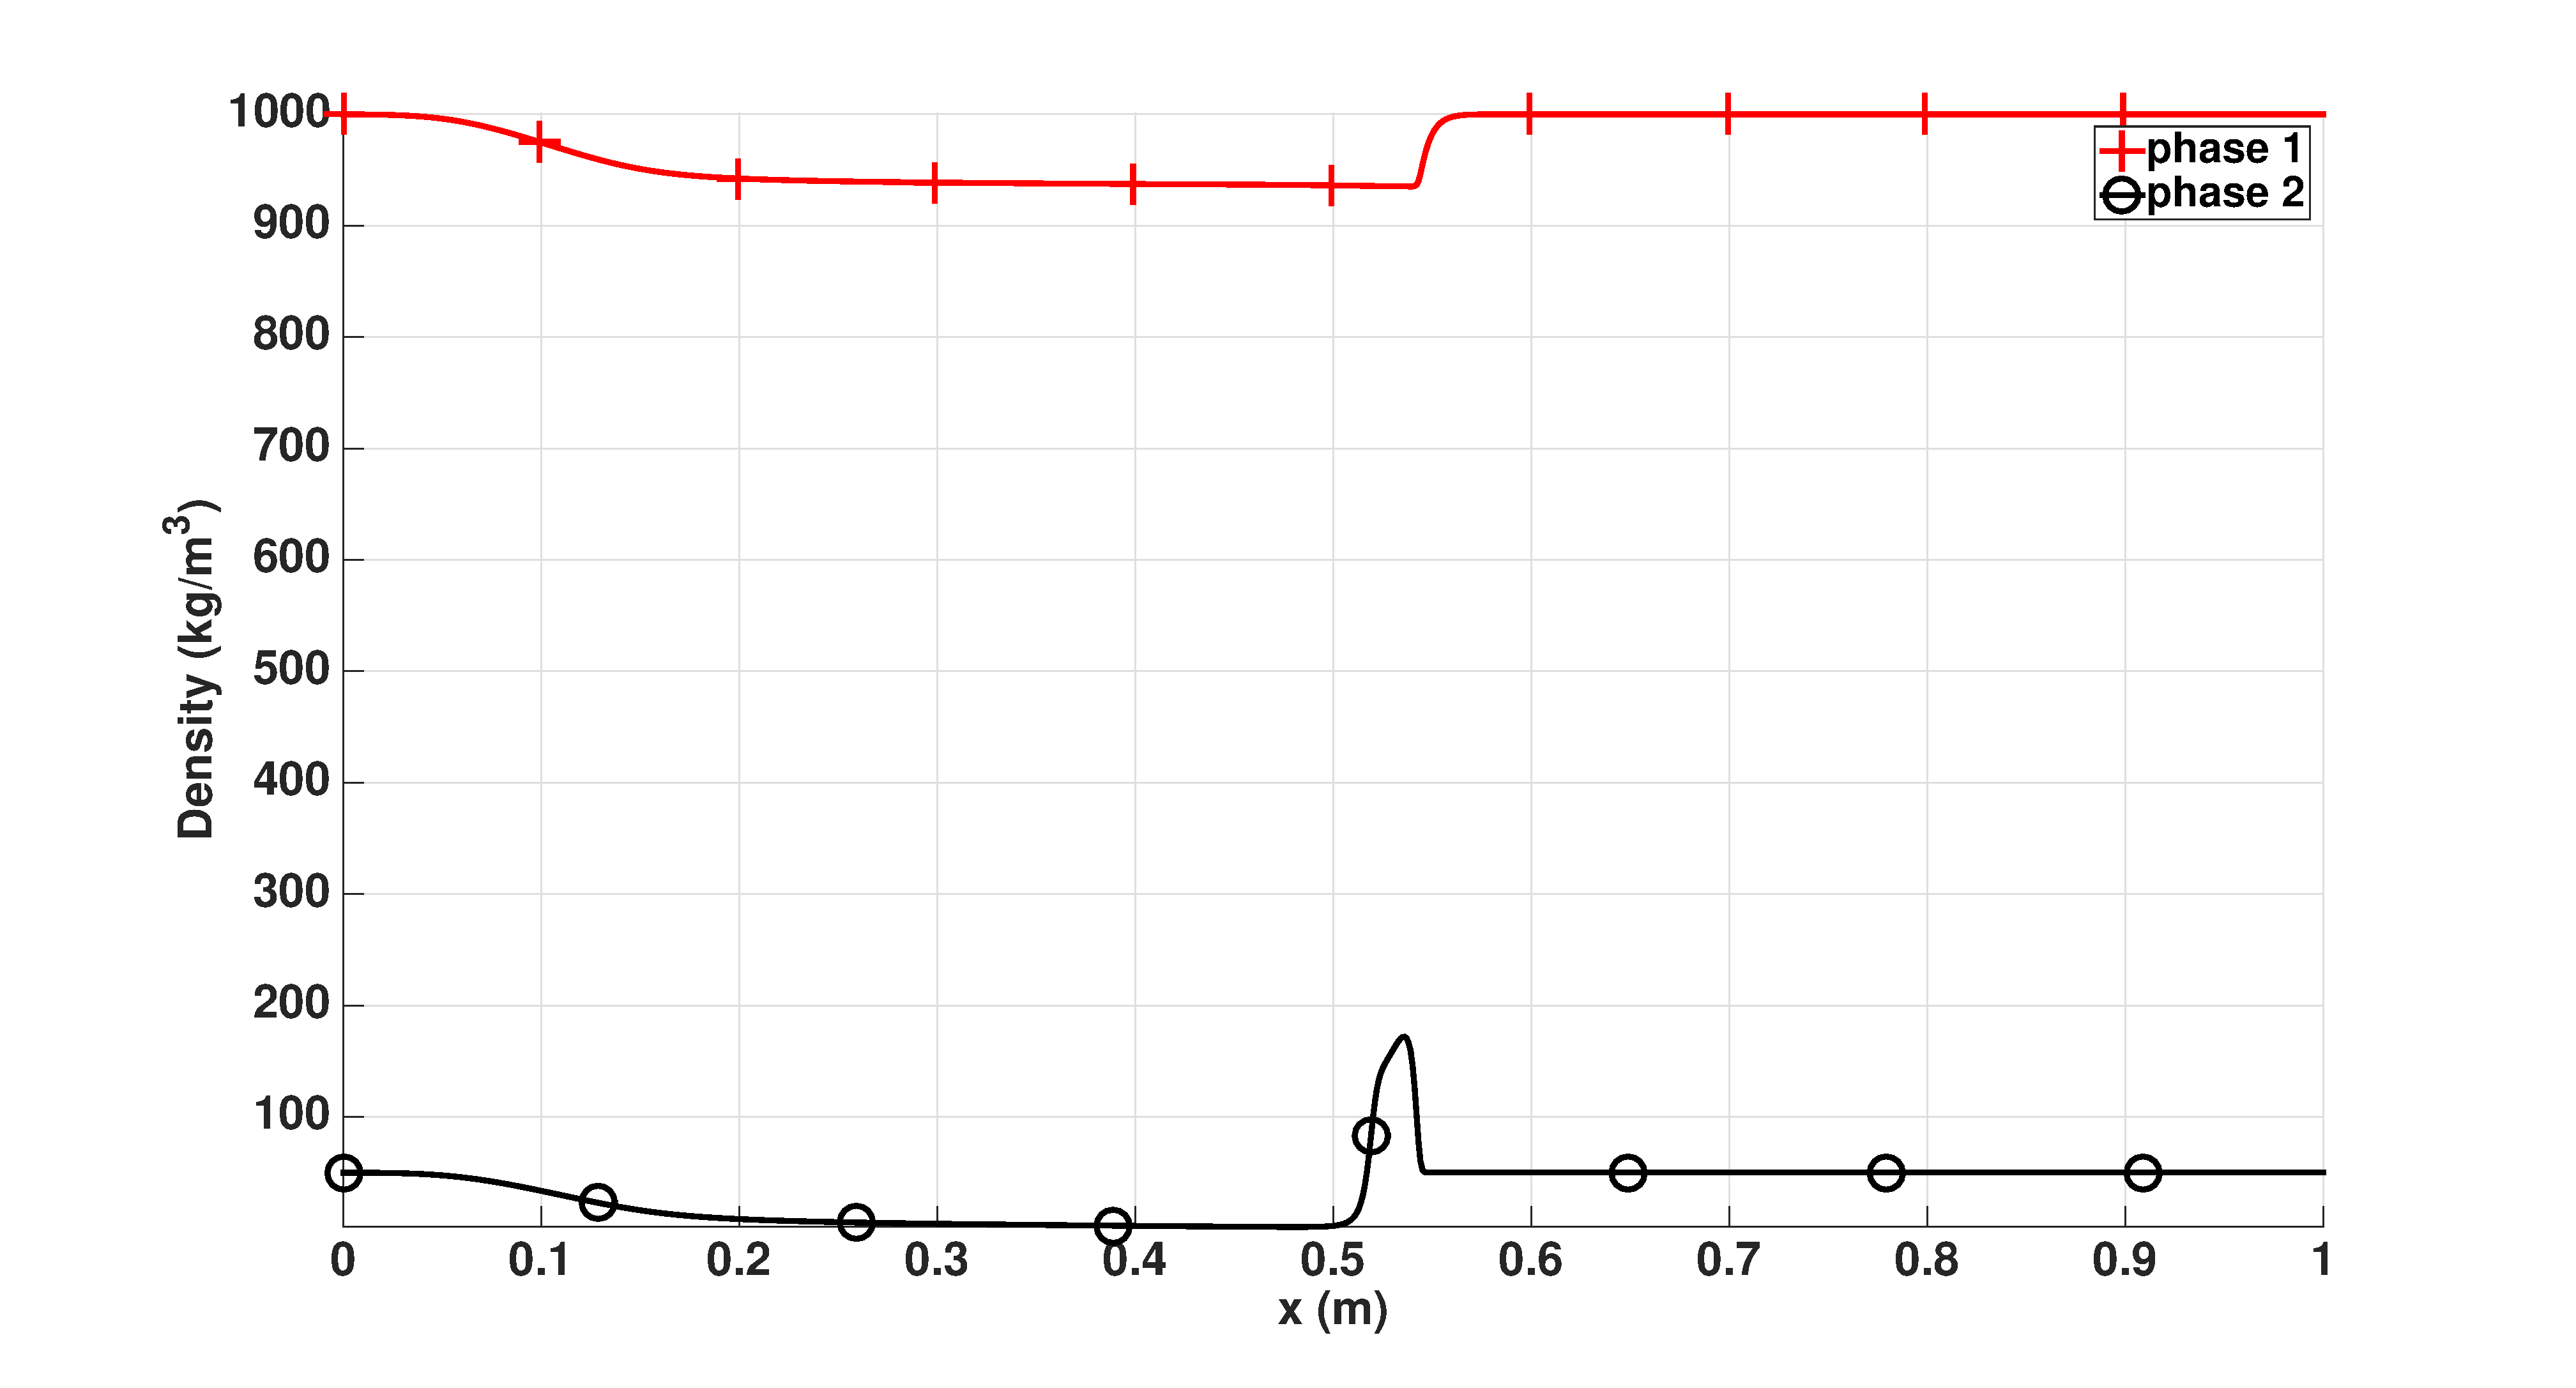
\includegraphics[width=\textwidth]{figures/pure_fluids_infinite_relaxation_two_phases_density.eps}
                \caption{Densities}
                \label{fig:nearly_pure_density}
        \end{subfigure}
        \caption{Nearly pure problem.}\label{fig:nearly_pure}
\end{figure}

%%%%%%%%%%%%%%%%%%%%%%%%%%%%%%%%%%%%%%%%%%%%%%%%%%%%%%%%%%%%%%%%%%%%%%%%%%%%%%%%%%%%%%%
\section{Conclusions}\label{sec:conclusion}
%%%%%%%%%%%%%%%%%%%%%%%%%%%%%%%%%%%%%%%%%%%%%%%%%%%%%%%%%%%%%%%%%%%%%%%%%%%%%%%%%%%%%%%
%%%%%%%%%%%%%%%%%%%%%%%%%%%%%%%%%%%%%%%%%%%%%%%%%%%%%%%%%%%%%%%%%%%%%%%%%%%%%
%
We have derived a viscous regularization for the hyperbolic Seven-Equation two-phase flow Model. 
The regularization ensures nonnegativity of the phasic entropy residual, 
convergence of the numerical solution to an entropy solution for concave phasic entropy functions $s_k$,
and is consistent with the viscous regularization derived for Euler equations when one of the phases disappears. 
We have also demonstrated that the proposed viscous regularization is compatible with the generalized Harten entropies 
that were initially derived for Euler equations. 

The viscous regularization for the SEM equations involves a set of two positive viscosity coefficients for each phase, $\mu_k$ and $\kappa_k$, and one for the volume 
fraction equation, $\beta_k$. Using non-dimensionalized equations, we have shown that the scaling of these viscosities is related to the numerical Reynolds 
and P\'eclet numbers, $\Re_k$, $\Pe_k^\mu$, and $\Pe_k^\kappa$. 
Adequate scaling of these numbers has been devised for two important limit-cases: the low-Mach asymptotic limit and for non-isentropic flows. In the low-Mach regime, 
we show that the incompressible equations are recovered when all of the non-dimensional numbers scale as one. The study of the non-isentropic case 
shows that the scaling of the non-dimensionalized numbers is Mach-number dependent to ensure well-scaled dissipative terms in the vicinity of the shock.
Based on these results, a proper scaling of the viscosity coefficients can be derived for all Mach numbers, as was the case for single-phase flows (see \cite{Marco_paper_low_mach}). 
%
We have also shown that the regularized SEM equations yields a regularized version of the five-equation flow model of Kapila by means of a Chapman-Enskog expansion.

The ability of the proposed regularization to stabilize the SEM equations was numerically demonstrated using a shock tube problem, with the definitions of the 
artificial viscosity coefficients borrowed from the local Lax-Friedrichs scheme. We have also performed a grid-convergence and analyzed the effect of removing 
stabilization from the volume fraction and the continuity equations. The scaling effect of the viscous regularization on the numerical solution in the low-Mach 
asymptotic limit was numerically illustrated using a 1-D converging-diverging nozzle. The proposed viscous regularization is agnostic of the spatial discretization
scheme and all of our numerical examples employed a {\it continuous} finite element method.

As an extension of this work, the two-phase flow viscous regularization presented here should be utilized and tested with high-order, less dissipative, artificial viscosities, 
such as the entropy viscosity (e.g., see \cite{jlg_EVM_JCP2011} for single-phase supersonic flows and \cite{Marco_paper_low_mach} for single-phase subsonic and transonic flows). 
We also note that the proposed regularization can also be employed using definitions of viscosity coefficients traditionally used in single-phase flows, e.g., 
the Lapidus viscosity \cite{Lapidus_paper,Lapidus_book} and pressure-based viscosity, for two-phase flows \cite{PBV_book}. We intend on reporting on these findings in 
a subsequent publication. 
%


%%%%%%%%%%%%%%%%%%%%%%%%%%%%%%%%%%%%%%%%%%%%%%%%%%%%%%%%%%%%%%%%%%%%%%%%%%%%%


\begin{acknowledgements}
The authors (M.D. and J.R.) would like to thank Bojan Popov and Jean-Luc Guermond for many fruitful discussions.  
This research was carried out under the auspices of the Idaho National Laboratory, a contractor of the U.S. Government under contract No. DEAC07-05ID14517.  Accordingly, the U.S. Government retains a non-exclusive, royalty-free license to publish or reproduce the published form of this contribution, or allow others to do so, for U.S. Government purposes.
\end{acknowledgements}

% BibTeX users please use one of
%\bibliographystyle{spbasic}      % basic style, author-year citations
\bibliographystyle{spmpsci}      % mathematics and physical sciences
%\bibliographystyle{spphys}       % APS-like style for physics
%%%%%%%%%%%%%%%%%%%%%%%%%%%%%%%%%%%%%%%%%%%%%%%%%%%%%%%%%%%%%%%%%%%%%%%%%%%%%
\bibliography{mybibfile}
%%%%%%%%%%%%%%%%%%%%%%%%%%%%%%%%%%%%%%%%%%%%%%%%%%%%%%%%%%%%%%%%%%%%%%%%%%%%%
\clearpage
%%%%%%%%%%%%%%%%%%%%%%%%%%%%%%%%%%%%%%%%%%%%%%%%%%%%%%%%%%%%%%%%%%%%%%%%%%%%%%
%%%%%%%%%%%%%%%%%%%%%%%%%%%%%%%%%%%%%%%%%%%%%%%%%%%
%
%  New template code for TAMU Theses and Dissertations starting Fall 2012.  
%  For more info about this template or the 
%  TAMU LaTeX User's Group, see http://www.howdy.me/.
%
%  Author: Wendy Lynn Turner 
%	 Version 1.0 
%  Last updated 8/5/2012
%
%%%%%%%%%%%%%%%%%%%%%%%%%%%%%%%%%%%%%%%%%%%%%%%%%%%

\begin{appendices}
%\titleformat{\chapter}{\centering\normalsize}{APPENDIX \thechapter}{0em}{\vskip .5\baselineskip\centering}
%\renewcommand{\appendixname}{APPENDIX}
%
%%%%%%%%%%%%%%%%%%%%%%%%%%%%%%%%%%%%%%%%%%%%%%%%%%%
%
%  New template code for TAMU Theses and Dissertations starting Fall 2012.  
%  For more info about this template or the 
%  TAMU LaTeX User's Group, see http://www.howdy.me/.
%
%  Author: Wendy Lynn Turner 
%	 Version 1.0 
%  Last updated 8/5/2012
%
%%%%%%%%%%%%%%%%%%%%%%%%%%%%%%%%%%%%%%%%%%%%%%%%%%%

%%%%%%%%%%%%%%%%%%%%%%%%%%%%%%%%%%%%%%%%%%%%%%%%%%%%%%%%%%%%%%%%%%%%%%
%%                           APPENDIX A 
%%%%%%%%%%%%%%%%%%%%%%%%%%%%%%%%%%%%%%%%%%%%%%%%%%%%%%%%%%%%%%%%%%%%%

\phantomsection

\section{Entropy equation for the multi-dimensional seven equation model without viscous regularization}\label{app:sev-equ-model-entropy}
%
This appendix provides the steps that lead to the derivation of the phasic entropy equation of the Seven-Equation two-phase flow Model \cite{SEM}. For the purpose of this appendix, two phases are considered with no interphase mass or heat transfer and denoted by the indexes $j$ and $k$. In the Seven-Equation two-phase flow Model, each phase obeys to the following set of equations (\eqt{eq:sev_equ-app}):
\begin{subequations}
\label{eq:sev_equ-app}
%
\begin{align}
\partial_t \left( \alpha_k  A\right) + A \mbold u_{int} \cdot \grad \alpha_k = A \mu_P \left( P_k - P_j \right) 
\end{align}
%
\begin{align}
\partial_t \left( \alpha_k \rho_k A \right) + \div \left( \alpha_k \rho_k \mbold u_k A \right) = 0 
\end{align}
%
\begin{multline}
\partial_t \left( \alpha_k \rho_k \mbold u_k A \right) + \div \left[ \alpha_k A \left( \rho_k \mbold u_k \otimes \mbold u_k + P_k \mathbb{I} \right) \right] =\\
\alpha_k P_k \grad A + P_{int} A \grad \alpha_k + A \lambda_u \left( \mbold u_j - \mbold u_k \right) 
\end{multline}
%
\begin{multline}
\partial_t \left( \alpha_k \rho_k E_k A \right) + \div \left[ \alpha_k A \mbold u_k \left( \rho_k E_k + P_k \right) \right] = \\
P_{int} A \mbold u_{int} \cdot \grad \alpha_k - A\mu_P \bar{P}_{int} \left( P_k-P_j \right) + \bar{\mbold u}_{int} A \lambda_u \left( \mbold u_j - \mbold u_k \right)
\end{multline}
\end{subequations}
where $\rho_k$, $\mbold u_k$, $E_k$ and $P_k$ denote the density, velocity, specific total energy, and pressure of  phase $k$, respectively. $\mu_P$ and $\lambda_u$ and the pressure and velocity relaxation parameters, respectively. We recall that we assume that the cross section $A$ is only function of space: $\partial_t A = 0$ (a value of $A \neq 1$ is mostly of practical important for 1D nozzle problems). 
Variables with subscript ${int}$ correspond to the interfacial variables; their definitions are given in \eqt{eq:sev_equ2-app}. 
\begin{equation}
\label{eq:sev_equ2-app}
\left\{
\begin{array}{lll}
P_{int} = \bar{P}_{int} - \frac{\grad \alpha_k}{|| \grad \alpha_k ||} \frac{Z_k Z_j}{Z_k + Z_j} \left( \mbold u_k-\mbold u_j \right) \\
\bar{P}_{int} = \frac{Z_k P_j + Z_j P_k}{Z_k + Z_j} \\
\mbold u_{int} = \bar{\mbold u}_{int} - \frac{\grad \alpha_k}{|| \grad \alpha_k ||} \frac{P_k - P_j}{Z_k + Z_j} \\
\bar{\mbold u}_{int} = \frac{Z_k \mbold u _k + Z_j \mbold u_j}{Z_k + Z_j}
\end{array}
\right.
\end{equation}
where $Z_k = \rho_k c_k$ and $Z_j = \rho_j c_j$ are the impedances of phases $k$ and $j$, respectively. The speed of sound is denoted by the symbol $c$. The sign function $sgn(x)$ returns $\pm 1$ according to the sign of variable $x$.

The first step in proving the entropy minimum principle for \eqt{eq:sev_equ-app} 
consists of recasting these equations using the primitive variables $(\alpha_k, \rho_k, \mbold u_k, e_k)$, where $e_k$ is the specific internal energy of phase $k$. We introduce the material derivative $\frac{D (\cdot)}{Dt} = \partial_t (\cdot) + \mbold u_k \cdot \grad (\cdot)$ for simplicity. 

The continuity equation can be expressed as follows:
\begin{equation}
\label{eq:cont1-app}
\alpha_k A \frac{D \rho_k}{Dt} + \rho_k A \mu_P \left( P_k-P_j \right) + \rho_k A \left( \mbold u_k-\mbold u_{int} \right) \cdot \grad \alpha_k + \rho_k \alpha_k \div \left( A \mbold u_k \right) = 0 \,.
\end{equation}
The momentum and continuity equations are combined to yield an equation for the velocity:
\begin{equation}
\label{eq:vel1-app}
\alpha_k \rho_k A \frac{D\mbold u_k}{Dt} + \grad \left( \alpha_k A P_k \right) = \alpha_k P_k \grad A + P_{int} A \grad \alpha_k + A \lambda_u \left( \mbold u_j-\mbold u_k \right) \,.
\end{equation}
A kinetic energy equation is obtained by multiplying the previous result by $\mbold u_k$ to yield:
\begin{multline}
\label{eq:kin1-app}
\alpha_k \rho_k A \frac{D\left(\mbold u_k^2/2\right)}{Dt} + \mbold u_k \grad \left( \alpha_k A P_k \right) = \\ \mbold u_k  \Big( \alpha_k P_k \grad A + P_{int} A \grad \alpha_k + A \lambda_u \left( \mbold u_j-\mbold u_k \right) \Big) \,.
\end{multline}
%
The internal energy equation is obtained by subtracting the above kinetic energy equation from the total energy equation:
\begin{multline}\label{eq:internal1}
\alpha_k \rho_k A \frac{D e_k}{Dt} + \alpha_k P_k \div \left(A \mbold u_k \right) = 
 P_{int} A \left(\mbold u_{int}-\mbold u_k \right) \cdot \grad \alpha_k \\
 - \bar{P}_{int} A \mu_P \left(P_k-P_j \right) + A \lambda_u \left(\mbold u_j-\mbold u_k  \right) \cdot \left(\bar{\mbold u}_{int}-\mbold u_k \right) \,.
\end{multline}

In the next step, we assume the existence of a phasic entropy $s_k$ that is function of the density $\rho_k$ and the  internal energy $e_k$. Using the chain rule, 
\begin{equation}
\frac{Ds_k}{Dt} = (s_\rho)_k \frac{D \rho_k}{Dt} + (s_e)_k \frac{De_k}{Dt},
\end{equation}
we combine the density and internal energy equations ($\rho_k (s_\rho)_k \times \eqt{eq:cont1-app}  + (s_e)_k \times \eqt{eq:internal1}$) to obtain  the following entropy equation :
\begin{multline}
\label{eq:ent1}
\alpha_k \rho_k A \frac{Ds_k}{Dt} + 
\underbrace{\alpha_k \left( P_k (s_e)_k + \rho_k^2 (s_\rho)_k \right)  \div \left( A \mbold u_k \right) }_\textrm{(a)} = \\
(s_e)_k A \left[ P_{int}(\mbold u_{int}-\mbold u_k)\cdot \grad \alpha_k - \bar{P}_{int} A \mu_P (P_k-P_j) + A \lambda_u (\bar{\mbold u}_{int}-\mbold u_k) \cdot (\mbold u_j-\mbold u_k)\right] \\
- \rho_k^2 (s_\rho)_k \left[ \mu_P A (P_k-P_j) + A(\mbold u_k-\mbold u_{int}) \cdot \grad \alpha_k\right] 
\end{multline}
where $(s_e)_k$ and $(s_\rho)_k$ denote the partial derivatives of entropy $s_k$ with respect to the internal energy $e_k$ and the density $\rho_k$, respectively.
The term denoted by (a) on the left-hand side of \eqt{eq:ent1} can be set to zero by invoking the second law of thermodynamics:
\begin{equation}
T_k ds_k = de_k - \frac{P_k}{\rho_k^2} d \rho_k \text{ with } (s_e)_k = \frac{1}{T_k} \text{ and } (s_\rho)_k = - \frac{P_k}{\rho_k^2} (s_e)_k
\end{equation}
which yields
\begin{equation}
\label{eq:ent2}
 P_k (s_e)_k + \rho_k^2 (s_\rho)_k = 0 .
\end{equation} 
% The above equation is equivalent to the application of the second law of thermodynamic law when assuming reversibility:

Finally,\eqt{eq:ent1} is as follows:
\begin{eqnarray}
\label{eq:ent3}
((s_e)_k)^{-1} \alpha_k \rho_k \frac{Ds_k}{Dt} = \underbrace{\left[ P_{int} (\mbold u_{int}-\mbold u_k) + P_k (\mbold u_k-\mbold u_{int}) \right] \cdot \grad \alpha_k}_\textrm{(b)} + \nonumber\\ 
\underbrace{\mu_P (P_k-P_j)(P_k-\bar{P}_{int})}_\textrm{(c)} + \underbrace{\lambda_u(\mbold u_j-\mbold u_k)\cdot(\bar{\mbold u}_{int}-\mbold u_k)}_\textrm{(d)}
\end{eqnarray}
The right-hand side of \eqt{eq:ent3} has been split into three terms, (b), (c), and (d); next we analyze each of these terms separately. The terms (c) and (d) can be easily recast by using the definitions of $\bar{\mbold u}_{int}$ and $\bar{P}_{int}$ given in \eqt{eq:sev_equ2-app}:
\begin{eqnarray}
\label{eq:ent4}
\mu_P (P_k-P_j)(P_k-\bar{P}_{int}) = \mu_P \frac{Z_k}{Z_k+Z_j} (P_j - P_k)^2\nonumber\\
\lambda_u(\mbold u_j-\mbold u_k)\cdot(\bar{\mbold u}_{int}-\mbold u_k) = \lambda_u \frac{Z_j}{Z_k+Z_j} (\mbold u_j - \mbold u_k)^2 
\end{eqnarray}
By definition, $\mu_P$, $\lambda_u$ and $Z_k$ are all positive. Thus, the above terms (c) and (d) are unconditionally positive. 

We now inspect term (b). Once again, we use the definitions of $P_{int}$ and $\mbold u_{int}$ and the following relations:
\begin{eqnarray}
\label{eq:ent4bis}
\mbold u_{int}-\mbold u_k &=& \frac{Z_j}{Z_k+Z_j}(\mbold u_j-\mbold u_k) -  \frac{\grad \alpha_k}{\| \grad \alpha_k \|} \frac{Pk-P_j}{Z_k+Z_j} \nonumber\\
P_{int}-P_k &=& \frac{Z_k}{Z_k+Z_j} (P_j-P_k) - \frac{\grad \alpha_k}{\| \grad \alpha_k \|} \frac{Z_k Z_j}{Z_k+Z_j} (\mbold u_k-\mbold u_j), \nonumber 
\end{eqnarray}
Then, term (b) becomes:
\begin{multline}
\label{eq:ent5}
\left[ P_{int} (\mbold u_{int}-\mbold u_k) + P_k (\mbold u_k-\mbold u_{int}) \right] \cdot \grad \alpha_k = (P_{int}-P_k)(\mbold u_{int}-\mbold u_k)\cdot \grad \alpha_k=   \\ 
\frac{Z_k}{\left( Z_k+Z_j \right)^2} \grad \alpha_k \cdot \left[ Z_j (\mbold u_j-\mbold u_k)(P_j-P_k)+\frac{\grad \alpha_k}{\| \grad \alpha_k \|} Z_j^2 (\mbold u_j-\mbold u_k)^2 \right. + \\ 
\left. \frac{\grad \alpha_k}{\| \grad \alpha_k \|}(P_k-P_j)^2 +  \frac{\grad \alpha_k \cdot \grad \alpha_k}{\| \grad \alpha_k \|^2}(P_k-P_j)Z_j (\mbold u_k-\mbold u_j) \right] 
\end{multline}
The above equation is factorized by $\|  \grad \alpha_k \|$ and then recast under a quadratic form using $\frac{\grad \alpha_k \cdot \grad \alpha_k}{\| \grad \alpha_k \|^2} = 1$. This yields:
\begin{align}
\label{eq:ent6}
\left[ (\mbold u_{int}-\mbold u_k)P_{int} + (\mbold u_k-\mbold u_{int})P_k \right] \grad \alpha_k &=  \nonumber \\
\| \grad \alpha_k \| \frac{Z_k }{\left( Z_k+Z_j \right)^2} \left[ Z_j (\mbold u_j-\mbold u_k) + \frac{\grad \alpha_k}{\| \grad \alpha_k \|}(P_k-P_j)\right]^2
\end{align}
Thus, using \eqt{eq:ent3}, \eqt{eq:ent4}, \eqt{eq:ent5} and \eqt{eq:ent6}, the entropy equation obtained in \cite{SEM} holds and is recalled here for convenience:
\begin{align}
(s_{e})_k^{-1} \alpha_k \rho_k A \frac{Ds_k}{Dt} &= \mu_P \frac{Z_k}{Z_k+Z_j} (P_j - P_k)^2 + \lambda_u \frac{Z_j}{Z_k+Z_j} (\mbold u_j -\mbold  u_k)^2 \nonumber
\\
& \| \grad \alpha_k \| \frac{Z_k}{\left( Z_k+Z_j \right)^2} \left[ Z_j (\mbold u_j-\mbold u_k)+\frac{\grad \alpha_k}{\| \grad \alpha_k \|}(P_k-P_j)\right]^2. \nonumber
\end{align}
%
\pagebreak{}
%%%%%%%%%%%%%%%%%%%%%%%%%%%%%%%%%%%%%%%%%%%%%%%%%%%
%
%  New template code for TAMU Theses and Dissertations starting Fall 2012.  
%  For more info about this template or the 
%  TAMU LaTeX User's Group, see http://www.howdy.me/.
%
%  Author: Wendy Lynn Turner 
%	 Version 1.0 
%  Last updated 8/5/2012
%
%%%%%%%%%%%%%%%%%%%%%%%%%%%%%%%%%%%%%%%%%%%%%%%%%%%

%%%%%%%%%%%%%%%%%%%%%%%%%%%%%%%%%%%%%%%%%%%%%%%%%%%%%%%%%%%%%%%%%%%%%%
%%                           APPENDIX B
%%%%%%%%%%%%%%%%%%%%%%%%%%%%%%%%%%%%%%%%%%%%%%%%%%%%%%%%%%%%%%%%%%%%%
%
\section{Compatibility of the viscous regularization for the seven-equation two-phase model with the generalized Harten entropies}\label{app:harden}
%
We investigate in this appendix whether the viscous regularization of the seven-equation two-phase model derived in \sct{sec:visc-regu} is compatible with some or all generalized entropies identified in Harten et al. \cite{Harten}. Considering the single-phase Euler equations, Harten et al. \cite{Harten} demonstrated that a function $\rho \mathscr{H}(s)$ is called a generalized entropy and is strictly concave if $\mathscr{H}$ is twice differential and
%
\begin{multline}\label{eq:generalized_ent}
\mathscr{H}' (s)  \geq 0, \ \ \ \ \mathscr{H}'(s)c_p^{-1} - \mathscr{H}'' \geq 0, \ \forall \left( \rho, e \right) \in \mathbb{R}_+^2 \ ,
\end{multline}
%
where $c_p \left( \rho, e \right) = T \partial_T s \left( \rho, e \right)$ is the specific heat at constant pressure ($T$ is a function of $e$ and $\rho$ through the equation of state). Because the seven-equation two-phase model was initially derived by assuming that each phase obeys the single-phase Euler equation, we want to investigate whether the above property still holds when considering the seven-equation model with viscous regularization included. To do so, we consider a phasic generalized entropy, $\mathscr{H}_k(s_k)$ and a phasic specific heat at constant pressure, $c_{p,k} \left( \rho_k, e_k \right) = T_k \partial_{T_k} s_k \left( \rho_k, T_k \right)$ characterized by \eqt{eq:generalized_ent}. The objective is to find an entropy inequality verified by $\rho_k \mathscr{H}_k(s_k)$.

We start from the entropy inequality verified by $s_k$, 
%
\begin{multline}\label{eq:ent-res-7-eqn-diss-terms-app}
\alpha_k \rho_k A \frac{Ds_k}{Dt} =  \mbold f_k \cdot \grad s_k + \div \left( \alpha_k A \rho_k \kappa_k  \grad s_k \right)  
- \alpha_k \rho_k A \kappa_k Q_k \\ + (s_e)_k \alpha_k A \rho_k \mu_k \grad^s \mbold u_k : \grad \mbold u_k.
\end{multline}
%
\eqt{eq:ent-res-7-eqn-diss-terms-app} is multiplied by $\mathscr{H}_k'(s_k)$ to yield:
%
\begin{multline}
\label{eq:ent-res-7-eqn-diss-terms-app2}
\alpha_k \rho_k A \frac{D\mathscr{H}_k(s_k)}{Dt} = \div \left( \alpha_k A \rho_k \kappa_k \grad \mathscr{H}_k (s_k) \right) - \mathscr{H}_k''(s_k) \alpha_k A \kappa_k \rho_k \| \grad s_k \|^2 + \\
\mathscr{H}_k'(s_k) \mbold f_k \cdot \grad s_k - \mathscr{H}_k'(s_k)\alpha_k \rho_k A \kappa_k Q_k +  \\
\mathscr{H}_k'(s_k)(s_e)_k \alpha_k A \rho_k \mu_k \grad^s \mbold u_k : \grad \mbold u_k 
\end{multline}
%
Let us now multiply the continuity equation of phase $k$ by $\mathscr{H}_k (s_k)$ and add the result to the above equation to obtain:
%
\begin{align}\label{eq:ent-res-7-eqn-diss-terms-app3}
\partial_t \left( \alpha_k \rho_k A \mathscr{H}_k(s_k)\right) + \div \left( \alpha_k \rho_k \mbold u_k A \mathscr{H}_k(s_k) \right)  &- \nonumber\\
\div \left[ \alpha_k A \rho_k \kappa_k \grad \mathscr{H}_k (s_k) + \alpha_k A \kappa_k \mathscr{H}_k (s_k) \grad \rho_k  \right. & \left. + A \kappa_k \rho_k \mathscr{H}_k (s_k) \grad \alpha_k\right] = \nonumber \\
\underbrace{-\mathscr{H}_k''(s_k) \alpha_k A \kappa_k \rho_k \| \grad s_k \|^2  - \mathscr{H}_k'(s_k) \alpha_k A \kappa_k \rho_k  Q_k}_{\mathbb{T}_0} &+\nonumber \\
\underbrace{ \mathscr{H}_k'(s_k)(s_e)_k  \alpha_k A \rho_k \mu_k \grad^s \mbold u_k : \grad \mbold u_k}_{\mathbb{T}_1} & .
\end{align}
%
As in \sct{sec:visc-regu}, the left-hand side of \eqt{eq:ent-res-7-eqn-diss-terms-app3} is split into two residuals denoted by $\mathbb{T}_0$ and $\mathbb{T}_1$ in order to study the sign of each of them. We start by studying the sign of $\mathbb{T}_1$ that is positive since it is assumed that $ \mathscr{H}_k'(s_k) \geq 0$. We now investigate the sign of $\mathbb{T}_0$. Using \eqt{eq:generalized_ent}, we have:
%
\begin{equation}\label{eq:new_quad_form}
- \mathbb{T}_0 \leq \mathscr{H}_k'(s_k) \alpha_k A \kappa_k \rho_k \left( c_{p,k}^{-1} \|\grad s_k\|^2 +  Q_k\right) \ .
\end{equation}
%
The right-hand side of \eqt{eq:new_quad_form} is a quadratic form that was already defined in Appendix 5 of \cite{jlg} and can be recast in the matrix form $X^t_k \mathbb{S} X_k$ where $\mathbb{S}$ is a $2 \times 2$ matrix and the vector $X_k$ was previously defined in \sct{sec:visc-regu}. In \cite{jlg}, matrix $\mathbb{S}$ is shown to be negative semi-definite which allows us to conclude that $\mathbb{T}_0$ is unconditionally positive using \eqt{eq:new_quad_form}. Then, knowing the sign of the two residuals $\mathbb{T}_0$ and $\mathbb{T}_1$, we conclude that:
%
\begin{align}\label{eq:ent-res-7-eqn-diss-terms-app4}
\partial_t \left( \alpha_k \rho_k A \mathscr{H}_k(s_k)\right) + \div \left( \alpha_k \rho_k \mbold u_k A \mathscr{H}_k(s_k) \right)  &- \nonumber\\
\div \left[ \alpha_k A \rho_k \kappa_k \grad \mathscr{H}_k (s_k) + \alpha_k A \kappa_k \mathscr{H}_k (s_k) \grad \rho_k  \right. & \left. + A \kappa_k \rho_k \mathscr{H}_k (s_k) \grad \alpha_k\right] \geq 0 \ .\nonumber 
\end{align}
%
For there, we conclude that an entropy inequality is satisfied for all generalized entropies $\rho_k \mathscr{H}_k (s_k)$ when using the viscous regularization derived in \sct{sec:visc-regu} for the seven-equation two-phase model. Note that the above inequality holds for the total entropy of the system as well, i.e., when summing over the phases (the source terms are determined from rational thermodynamics that requires summations over the phases).
%
\pagebreak{}
%
\end{appendices}
%%%%%%%%%%%%%%%%%%%%%%%%%%%%%%%%%%%%%%%%%%%%%%%%%%%%%%%%%%%%%%%%%%%%%%%%%%%%%%



\end{document}
% end of file template.tex

